\PassOptionsToPackage{italian,english}{babel}
\documentclass[12pt,a4paper,oneside,openright]{book}

\setcounter{secnumdepth}{3} % it actually equals to 4 levels of depth numbering
% for example 1.1.1.1 (equivalent to a subsubsection)

\usepackage{packages} % inserisce tutti le macro necessarie per il
                        % funzionamento
\usepackage{frontesp} % modificare questo file per i diplomi e se si ha
                        % un solo correlatore
\usepackage{setspace}
\usepackage[utf8]{inputenc}
\usepackage[english]{babel}
\usepackage{graphicx}
\usepackage{booktabs}
\usepackage{amssymb}
\usepackage{amsmath}
\usepackage{amsthm}
\usepackage{url}
\usepackage{xspace}
\usepackage[margin=2.5cm]{geometry}
\usepackage{tikz}
\usetikzlibrary{positioning,calc,matrix,arrows}
\usepackage{pgfplots}
\usepackage{listings}
\usepackage{color}
\usepackage{textcomp}
\usepackage{fancyvrb}
\usepackage{array}

\usepackage{float} %instance segm
\usepackage{tabularx} %modanet
\usepackage{placeins} %floatbarrier
\usepackage[super]{nth} % paperdoll release date and dates in general

%\usepackage[colorlinks]{hyperref}
\usepackage[colorlinks,plainpages=false,hyperindex,bookmarksopen,linkcolor=black,citecolor=black,urlcolor=black]{hyperref}
\usepackage{cleveref}



\let\oldquote\quote
\let\endoldquote\endquote
\renewenvironment{quote}[2][]
{\if\relax\detokenize{#1}\relax
	\def\quoteauthor{#2}%
	\else
	\def\quoteauthor{#2~---~#1}%
	\fi
	\oldquote}
{\par\nobreak\smallskip\hfill(\quoteauthor)%
	\endoldquote\addvspace{\bigskipamount}}


% Example usage of quote:
%\begin{quote}[Somewhere]{Somebody}
%	This is a quote This is a quote This is a quote
%	This is a quote This is a quote This is a quote
%	This is a quote This is a quote This is a quote
%\end{quote}


\newtheorem{example}{Example}
\newtheorem{lemma}{Lemma}

\newcommand{\real}{\mathbb{R}}
\newcommand{\vv}{\operatorname{vec}}
\newcommand{\diag}{\operatorname{diag}}
\newcommand{\matconvnet}{\textsc{MatConvNet}\xspace}
\newcommand{\matlab}{\textsc{MATLAB}\xspace}
\newcommand{\cpp}{C{}\texttt{++}~}
\newcommand{\bx}{\mathbf{x}}
\newcommand{\by}{\mathbf{y}}
\newcommand{\bc}{\mathbf{c}}
\newcommand{\bz}{\mathbf{z}}
\newcommand{\bff}{\mathbf{f}}
\newcommand{\bg}{\mathbf{g}}
\newcommand{\br}{\mathbf{r}}
\newcommand{\bw}{\mathbf{w}}
\newcommand{\bp}{\mathbf{p}}
\newcommand{\bfs}{\mathbf{s}}
\newcommand{\bfe}{\mathbf{e}}
\newcommand{\bone}{\mathbf{1}}
\newcommand{\argmin}{\operatornamewithlimits{argmin}}
\newcommand{\argmax}{\operatornamewithlimits{argmax}}
\newcommand{\sign}{\operatornamewithlimits{sign}}
\newcommand{\maskrcnn}{\textsc{Mask R-CNN} [\sref{s:maskrcnn}]\xspace}
\newcommand{\modanet}{\textsc{ModaNet} [\sref{s:ds-modanet}]\xspace}

% adding page numbers to references! (just run it two times if you see "??")
\newcommand*{\fref}[1]{Fig.~\ref{#1}  (p.~\pageref{#1})} %figure
\newcommand*{\eref}[1]{Eq.~\ref{#1}  (p.~\pageref{#1})} %equation
\newcommand*{\tref}[1]{Table~\ref{#1}  (p.~\pageref{#1})} %table
\newcommand*{\sref}[1]{\cref{#1}  (p.~\pageref{#1})} %section

\tikzstyle{block} = [draw, rectangle, minimum height=3em, minimum width=3em]
\tikzstyle{data} = []
\tikzstyle{datac} = [draw, circle, minimum height=2.5em, minimum width=2.5em,inner sep=3pt,font=\footnotesize]
\tikzstyle{par} = [draw, circle, minimum height=2.5em, minimum width=2.5em,fill=black!20,inner sep=3pt,font=\footnotesize]
\tikzstyle{pinstyle} = [pin edge={to-,thin,black}]
\tikzstyle{to} = [->,>=stealth',shorten >=1pt,semithick]
\tikzstyle{from} = [<-,>=stealth',shorten >=1pt,semithick]
\tikzstyle{bp} = [draw=blue,text=blue]
\tikzstyle{bpl} = [draw=blue!40]
\tikzstyle{bpe} = [text=blue,draw=none]

\VerbatimFootnotes


\definecolor{listinggray}{gray}{0.9}
\definecolor{lbcolor}{rgb}{0.8,0.8,0.8}
\lstset{
	%backgroundcolor=\color{lbcolor},
	tabsize=4,
	rulecolor=,
	language=matlab,
	basicstyle=\small,
	upquote=true,
	columns=fullflexible,
	showstringspaces=false,
	extendedchars=true,
	breaklines=false,
	prebreak = \raisebox{0ex}[0ex][0ex]{\ensuremath{\hookleftarrow}},
	%frame=single,
	showtabs=false,
	showspaces=false,
	showstringspaces=false,
	identifierstyle=\ttfamily,
	keywordstyle=\color[rgb]{0,0,1},
	commentstyle=\itshape\color[rgb]{0.133,0.545,0.133},
	stringstyle=\color[rgb]{0.627,0.126,0.941},
}

\setstretch{1.3}  %interlinea, mettere 1 per singola da usarsi per le bozze!!!

\begin{document}

\begin{figure}
	\centering
	
\includegraphics[width=6cm]{images/logo.png}
\end{figure}

\title{Valutazione comparativa di segmentazione di istanze di abbigliamento}

\providecommand{\entitle}{Comparative evaluation of instance-based apparel segmentation}

\providecommand{\autore}{Pier Carlo Cadoppi}                        %candidato
\providecommand{\matricola}{276645}
\providecommand{\principaladviser}{Chiar.mo~Prof. Andrea Prati}  %relatore
\providecommand{\firstreader}{Leonardo Rossi}            %correlatore
%\providecommand{\secondreader}{Chiar.mo~Prof. R. SEMPRONIO}   %correlatore
\providecommand{\annoacc}{2018/19}
\providecommand{\tipo}{Triennale} % corso di laurea in ??
\providecommand{\corso}{Informatica, Elettronica e delle Telecomunicazioni} % corso di laurea in ??
\providecommand{\subtitle}{Detecting clothing and footwear in real world images} % sottotitolo?

% genera la prima pagina

\titlep

% indica l'inizio della parte introduttiva
\frontmatter

   \vspace*{10pc}
\thispagestyle{empty}
\begin{flushright}
\sl

Ringrazio IMP Lab per il template... :)

Poi ringrazio anche chi devo/voglio

\end{flushright}
\par\vfill\par

   \tableofcontents
   \listoffigures
   \listoftables
%   \listofalgorithms

\clearpage

% indica l'inizio della parte centrale
\mainmatter
 \chapter*{Abstract}
\markboth{Abstract}{Abstract}
%\addcontentsline{toc}{chapter}{Abstract}
\selectlanguage{english}
\section*{English Abstract}

The task I was given was detecting clothing and shoes in real world images -- the IMP Lab team had previously only trained the algorithms using studio quality images.

Apparel instance segmentation is composed of two tasks: finding the objects (instances), and drawing a line around them (segmentation). What previously had to be done by hand, now can be done automatically by a computer. This work allows for future implementation on, for example, Instagram -- the biggest social site for apparel images. We could track how a clothing item is used, where, and with whom. Or measure how well a Creator/Influencer is doing in promoting the products he/she was paid to wear.

What I did was use an existing neural network and search for a dataset to train it for detecing clothing on user generated images. This means that the program (for which I created a Command Line Interface) takes as input an image file (or a URL to an image) and returns a processed image; in which annotations such as whether the person is wearing pants, skirts, a dress, footwear or other labels are appended and shown, with a rectangular bounding box and a corresponding mask inside.

The dataset I found is called \modanet, and it is really based on the Paperdoll dataset. \modanet (by eBay researchers) has put annotations to this enormous dataset (about 1 million images)[but only 55k are annotated].

So the work I've done is integrating the dataset with the training algorithm. Fortunately, the \modanet annotations already used COCO's style, but the images were in an SQL database I had to extract (and then put the extraction program into a one-click CLI process!).
Then, I had to create another program that split the annotations into training, validation and test and organize them correctly. The first few weeks were very disappointing and it felt like combining this particular dataset was an impossible feat. It turned out that the lab computer Keras bad installation was also at fault.
Really the first assignment I was given, which I solved relatively quickly, was, using the default image provided and the default weights of \maskrcnn, to cut the image into several segments, each one showing only one object (annotation).

As for the splitting datasets annotations task, I made two revisions. The first one splitted by annotations but left some images in more than one set. So you could have had the same image on different sets but some annotations for that image were in one set and some in the other. This created confusion in the algorithm, but made the task of creating a heterogeneous and balanced training set easier. Second revision was the more classic (I then discovered) approach: putting an image in only one set, and with all its annotations. This made the task of keeping the sets balanced in terms of categories of labels on each set, but I made it!

After completing the first phase (i.e. the "making it work" one), I was advised to create a package for one-click install of the things I had done to make it work.

In the meantime, at dark times when I couldn't go forward without some advising, I let the computer do its things and run the training algorithms. The most I managed to keep it running was about 3-4 days (the computer was shared amongst other researchers and thesists). I managed to reach epoch 28, and I got quite nice results, even though it has a hard time recognizing both feet's footwear most of the time. 

I also made nice customizable viewing commands to see the processed images, and to quickly scan through the validation set (via the --set-all option) to see if the algorithm has improved or not based on your training.

I then fixed a longtime error -- many annotations gave a warning of "invalid indexes" during training because they went outside the images' borders. This way, the dataset got twice as big in an instant, so I decided to redo all the tests. I also discovered that many footwear annotations had been wrongly labeled, with overlapping bounding boxes and shapes belonging to more than one box. There are still cases of that happening now, but they have been almost halved.

This allowed the algorithm to better grasp footwear and boots, something it had never been able to do in months.
\pagebreak

\selectlanguage{italian}
\section*{Italian Abstract}


Il task che ho scelto era di riconoscere vestiti e scarpe in immagini scattate in condizioni naturali -- l'IMP Lab dell'Università con cui ho svolto questa tesi aveva fino ad ora solo addestrato gli algoritmi usando immagini di alta qualità e con sfondo uniforme.

Il problema di segmentazione di istanze di abbigliamento è diviso in due parti: trovare gli oggetti (instances), e contornarli (segmentation). Quello che prima doveva essere fatto a mano, ora piò essere fatto da un computer. Questa implementazione permette futuri lavori di applicazione su, per esempio, Instagram -- il social network più in voga oggi per condivisione di capi di abbigliamento. Si potrebbe analizzare ad esempio come un tipo di vestito è usato, in che contesto e con chi. O misurare l'impatto che gli Influencers hanno sui propri fan, in relazione agli oggetti che promuovono (e che sono pagati per promuovere).

Quello che ho fatto è usare un neural network esistente e cercare un dataset per fargli imparare a riconoscere abbigliamento in immagini generate da persone. Questo significa che il programma (per il quale ho creato una Command Line Interface) prende come input un file di immagine (o l'URL a un'immagine) e ritorna un'immagine processata; nella quale le annotazioni, come per esempio se una persona indossa pantaloni, gonne, un vestito o altri label, sono aggiunte all'immagine e mostrate all'utente. Con un bounding box rettangolare e una maschera corrispondente all'interno.

Il dataset che ho trovato si chiama \modanet, e si basa in realtà su Paperdoll.
\modanet (fatto da ricercatori di eBay) ha annotato più di 50mila immagini (anche se l'intero dataset consiste di quasi un milione di immagini).

Quindi il lavoro che ho fatto è stato integrare il dataset con l'algoritmo di training. Fortunatamente, le annotazioni \modanet seguivano già lo stile COCO, però le immagini erano compresse dentro a un database SQL che ho dovuto estrarre (e poi automatizzare questo processo nella CLI!). Successivamente, ho dovuto creare un altro programma per dividere le annotazioni in training, validation and test set, organizzandole correttamente.
Le prime settimane sono state davvero deludenti e sembrava che il dataset e il training proprio non volessero funzionare insieme. Alla fine abbiamo persino dovuto reinstallare Keras perchè era stato installato male! La prima cosa che mi era stata assegnata l'avevo in realtà risolta in fretta, ovvero dovevo usare un modello (già addestrato dai creatori di \maskrcnn per riconoscere alcuni oggetti in un'immagine) e invece che far vedere l'immagine intera annotata, far vedere soltanto le singole annotazioni una per una.

Per il programma di suddivione delle annotazioni, ho fatto due versioni. La prima le divideva per singole annotazioni, ma permetteva a un'immagine di appartenere a più dataset. Naturalmente con alcune annotazioni di quell'immagine in un set e altre nell'altro. La seconda (che ho poi scoperto essere il metodo classico) le suddivideva per immagini, quindi prendeva un'immagine e la metteva in un set, con tutte le sue annotazioni.

Dopo aver completato la prima fase, mi è stato suggerito di creare un package per permettere a chiunque di installare e rendere pronto all'uso il mio elaborato.
Nel frattempo che io cercavo di risolvere i problemi insormontabili, il computer lavorava per giorni per addestrare l'argoritmo sul dataset. Il massimo che sono riuscito a tenerlo a lavorare è 3-4 giorni (il PC è condiviso con altri tesisti). Sono riuscito a raggiungere l'epoca 28 e ho raggiunto ottimi risultati, nonostante qualche difficolta nel trovare scarpe e footwear.

Ho fatto anche utili comandi per vedere facilmente il risultato dando in pasto immagini manualmente o dal validation set.

Ho poi sistemato un errore che avevamo dato per perso: molte annotazioni venivano buttate via perchè uscivano, seppur di poco, dall'immagine. Dopo aver verificato che le annotazioni "invalide" erano corrette, le abbiamo ridimensionate per farle stare dentro all'immagine. Per questo avevo deciso di rifare i test per vedere i miglioramenti. I risultati dopo questo test erano quasi identici. Infatti il problema non era nelle annotazioni che andavano fuori dall'immagine, ma nei bounding box che erano sovrapposti e non seguivano le segmentazioni di scarpe e footwear. Ho quindi sistemato, per quanto possibile, le annotazioni e i bounding box sovrapposti sono stati dimezzati.

Grazie a quest'ultimo accorgimento, finalmente l'algoritmo è ora in grado di riconoscere correttamente tutte e 13 le categorie per cui è stato addestrato.



\selectlanguage{english}

 \chapter*{Introduction}
\markboth{Introduzione}{Introduzione}
\addcontentsline{toc}{chapter}{Introduzione}

Thesis introduction.

What I did was use an existing neural network and search for a dataset to train it for detecing clothing on user generated images. This means that the program (for which I created a Command Line Interface) takes as imput an image file (or a URL to an image) and returns a processed image; in which annotations such as whether the person is wearing pants, skirts, a dress, footwear or other labels are appended and shown, with a squared bounding box and a corresponding mask inside.

The dataset I found is called Modanet, and it is based off really the Paperdoll dataset. Modanet (by eBay researchers) has put annotations to this enormous dataset (about 1 million images)[but only  55k are annotated].

So the work I've done is integrating the dataset with the training algorithm. Fortunately, the Modanet annotations already used COCO's style, but the images were in an SQL database I had to extract (and then put the extraction program into a one-click CLI process!).
Then, I had to create another program that split the annotations into training, validation and test and organized them correctly. The first few weeks were very disappointing and it felt like combining this particular dataset was an impossible feat. It turned out that the lab computer Keras bad installation was also at fault.
Really the first assignment I was given, which I solved relatively quickly, was, using the default image provided and the default weights of MaskRCNN, to cut the image into several segments, each one showing only one object (annotation).

After completing the first phase (i.e. the "making it work" one), I was advised to create a package for one-click install of the things I had done to make it work.

In the meantime, at dark times when I couldn't go forward without some advising, I let the computer do its things and run the training algorithms. The most I managed to keep it running was about 3-4 days (the computer was shared amongst other researchers and thesists). I managed to reach epoch 28, and I got quite nice results, even though it has a hard time recognizing both feet's footwear most of the time. 

I also made nice customizable viewing commands to see the processed images, and to quickly scan through the validation set (via the --set-all option) to see if the algorithm has improved or not based on your training. % attenzione! guardare introd.tex per vedere come e' fatto
 \chapter{State of the art}
\label{stato dell'arte}


Capitolo uno: 
esempio di bibliografia \cite{2015arXiv150200046K}, un esempio di figura \fref{figure:test inserimento} e un esempio di tabella \tref{table:esempio_tabella}.

\begin{figure}[H]
	\centering
	\includegraphics[width=8cm]{images/example.png}
	\caption{Test inserimento immagini}
	\label{figure:test inserimento}
\end{figure}

\begin{table}[!htbp]
	\centering
	\begin{tabular}{l|l}
		\toprule
		Colonna 1 & Colonna 2 \\
		\midrule
		Valore 1 & Valore 2 \\
		Valore 3 & Valore 4 \\
		Valore 5 & Valore 6 \\
		\bottomrule
	\end{tabular}
	\caption{Descrizione della tabella}
	\label{table:esempio_tabella}
\end{table}


% ------------------------------------------------------------------
\section{Neural Networks}\label{s:fundamentals}
% ------------------------------------------------------------------

Neural Networks are becoming part of our life. All the apps we use are progressively adopting neural networks for pattern recognition and prediction.
In this section I'll provide an introduction to how they work and why a Neural Network was perfect for my task: recognizing clothing in a real world image.

% ------------------------------------------------------------------
\subsection{Introduction}\label{s:fund-intro}
% ------------------------------------------------------------------
\begin{quotation}
Machine Learning is a subfield of computer science focusing on programming computers to learn from data without being explicitly programmed. Machine learning algorithms learn and recognize patterns in seen data (training data) and use these patterns to predict characteristics of unseen data. \cite{IntroductiontoMachineLearningAlanZhengSeptember2018}
\end{quotation}

They can learn in 3 main ways:
\begin{enumerate}
	\item Supervised Learning:
		The algorithm is fed with annotations created by humans. It uses those to learn and grasp correlations between patterns, and apply them to newly fed images.
	\item Unsupervised Learning:
		It works the opposite way, trying to assign objects to groups, thus creating "unlabeled labels". So it groups all items with certain common patterns together.
	\item Reinforcement Learning:
		Reinforced Learning is commonly used to make computers learn how to play games. In Reinforced Learning, a goal is specified and the agent is given rewards for following a succesful path,
\end{enumerate}
For our purpose, I seeked to find a labeled dataset, because to recognize clothes and apparel we needed labeled images to let the algorithm know which is which.


Here are some basic words we need to know:
\begin{itemize}
	\item Label:
		The thing we're trying to predict. Ex: If we're trying to predict what kind of animal is in a picture, the label would be the type of animal in the picture.
	\item Classification:
		Taking each instance and assigning it to a particular category. Ex: Determining if tumors are benign or malignant by looking at MRI scans.
	\item Regression:
		Instead of having discrete classes, like classification, the "class" to be predicted is made up of continuous numerical values. Ex: Predicting house prices based on square footage, number of rooms, etc.
	\item Clustering:
		For data without pre-labeled classes, clustering is the act of grouping similar data points together. A form of unsupervised learning. Ex: Clustering U.S. households for marketing data.
	\item Training Data:
		The initial set of data used to discover potentially predictive relationships. It's what your machine learning algorithm "trains" on and learns patterns from.
	\item Validation and Testing Data:
		Set of data used to assess the strength and utility of predictive relationship. Your machine learning algorithm does not see this data during training.
	\item Error:
		The difference between algorithm's prediction and ground-truth values.
	\item Ground Truth:
		Data that is known to be correct. A data-set's labels.
	\item Features:
		The attributes of the data that are used to make a prediction about the labels. Ex: In the house price example in the regression definition, the features would be the square footage, number of rooms, etc.
	\item Feature space:
		The n-dimensions in which the features live where n = the number of features. Typically, the larger the feature space, the more complex your algorithm will be.
	\item Model:
		The relationship between features and label. Training means "learning" this relationship based on examples.


	
\end{itemize}
Let's briefly explain some concepts before diving into Neural Networks:

\subsubsection{Towards NNs}\label{s:fund-intro-tonn}
\begin{enumerate}
	\item Overfitting:
		\begin{figure}[H]
			\centering
			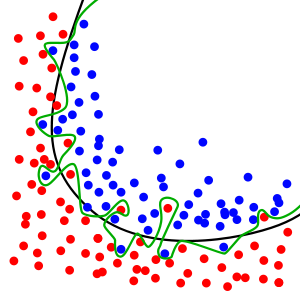
\includegraphics[scale=0.4]{images/overfitting.png}
			\caption{Overfitting on a simple separation problem}
			\label{f:overfitting}
		\end{figure}
		Simply put, overfitting means overgeneralizing narrow concepts. In the image above we can clearly see that the semantic line we should follow is the black one, even though, for this \emph{particular} dataset, the green line would produce the best results.
		What the green separation is doing is not grasping the shape of the separation, but picking up the intrinsic noise of real problems.
		
		\begin{figure}[H]
			\centering
			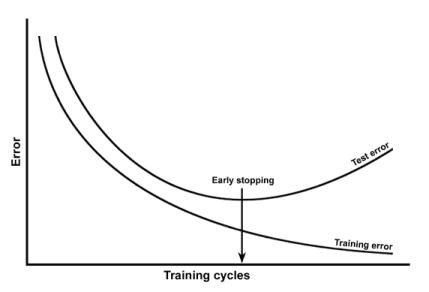
\includegraphics[scale=1.2]{images/overfittinglines.png}
			\caption{Recognizing overfitting}
			\label{f:overfittinglines}
		\end{figure}
		It's easy to recognize overfitting when training. If the error rates start to diverge, it usually is because of it. Avoiding it requires having a broad dataset that is balanced on the amount of annotations of each type.
	\item Decision Trees:
		
		They narrow down objects into classes by using binary questions repeatedly.
	\item Random Forests:
		
		A number of Decision Trees grouped together to identify multiple features.
		\begin{figure}[H]
			\centering
			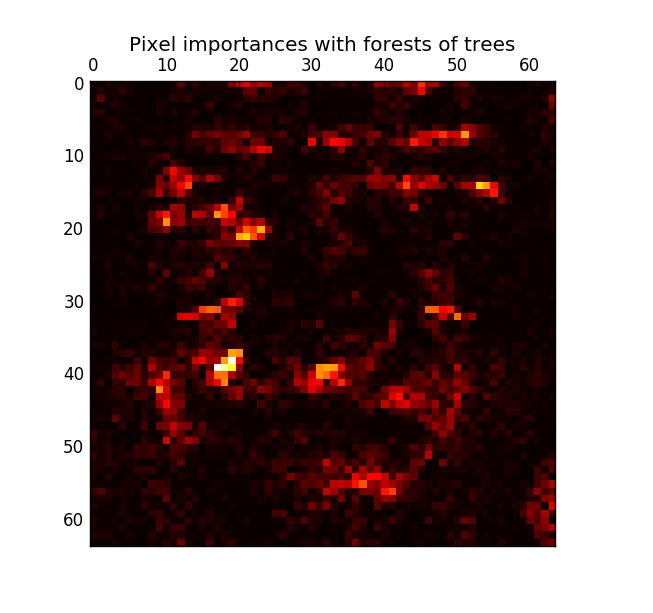
\includegraphics[scale=0.4]{images/featureimportance.jpg}
			\caption{Feature Importance using Random Trees}
			\label{f:featureimportance}
		\end{figure}
		They can be also used to measure the importance a particular feature. In fact, while usually the most important features in a tree are the top level ones, in random forests you have more than one tree, so a good way to find the importance of a feature is averaging the depth of the level where the feature is present in all the trees of the forest. In the image above, the features are the single pixels.
	\item Support Vector Machines:
	
		SVMs are widely used (\sref{s:nnevo-cnn}) to do supervised learning on both linear and non-linear classification.
		\begin{figure}[h!]
			\centering
			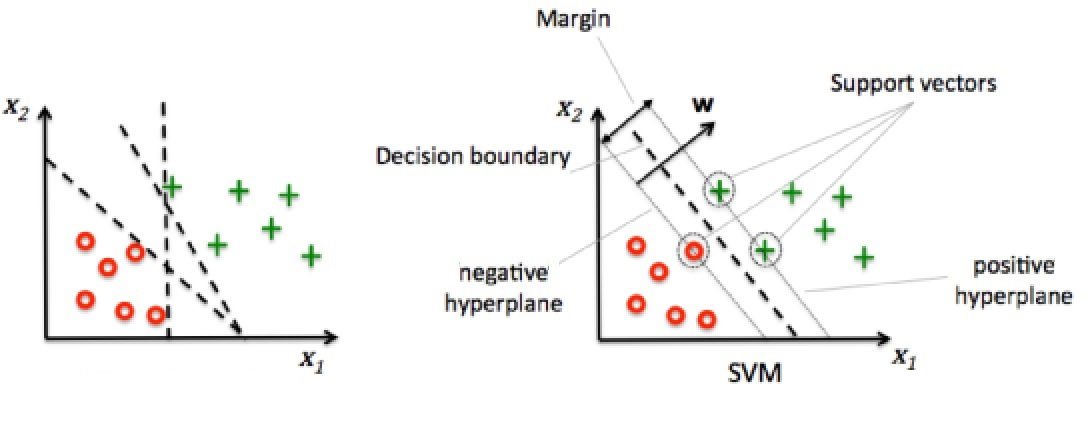
\includegraphics[scale=0.4]{images/svm.jpg}
			\caption{Linear Classification on Support Vector Machine}
			\label{fig:svm}
		\end{figure}
		\begin{figure}[h!]
			\centering
			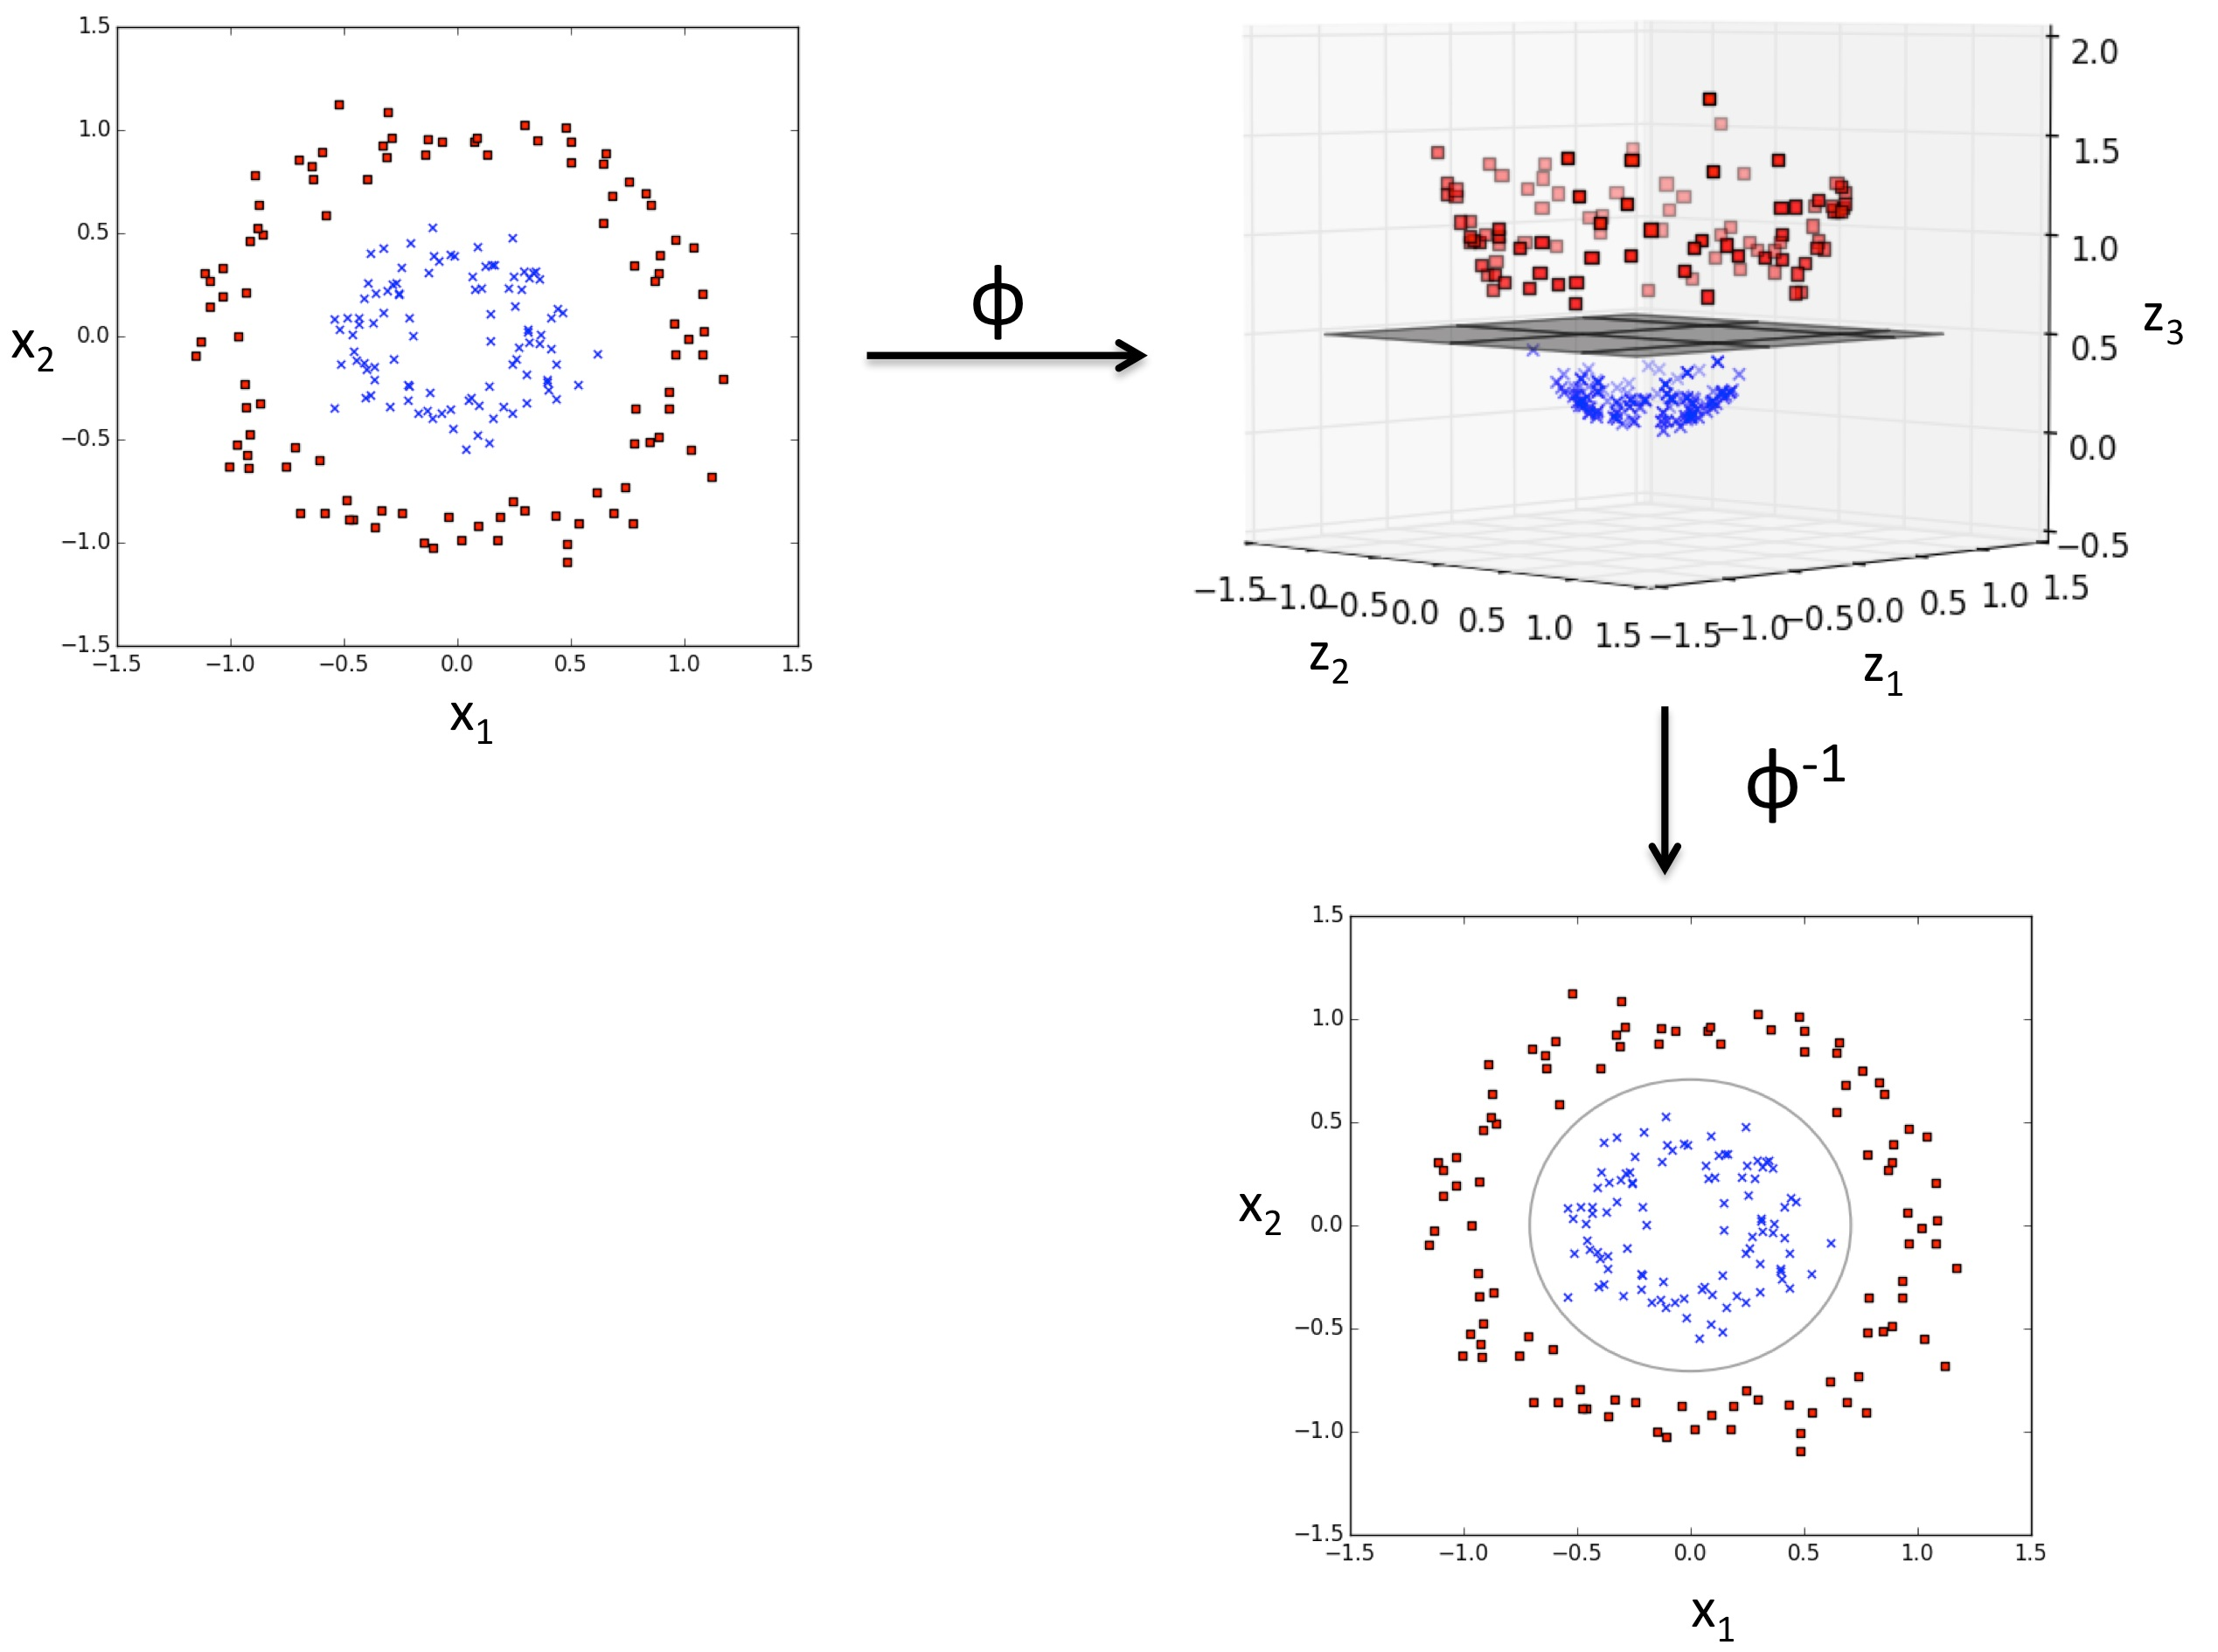
\includegraphics[scale=0.18]{images/dimensions.jpg}
			\caption{Non-Linear Classification on Support Vector Machine}
			\label{fig:mapping}
		\end{figure}
	\item Intersection over Union (IoU) for object detection:
		
		IoU is an evaluating method used to measure the accuracy of an object detector on a particular dataset.
		
		\begin{figure}[htbp]
			\centering
			\begin{minipage}{0.45\textwidth}
				\centering
				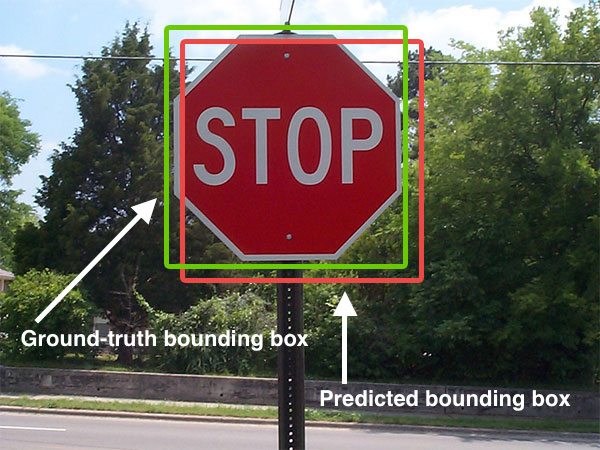
\includegraphics[width=0.8\textwidth]{images/iou_stop_sign.jpg} % first
				%figure itself
			\end{minipage}\hfill
			\begin{minipage}{0.45\textwidth}
				\centering
				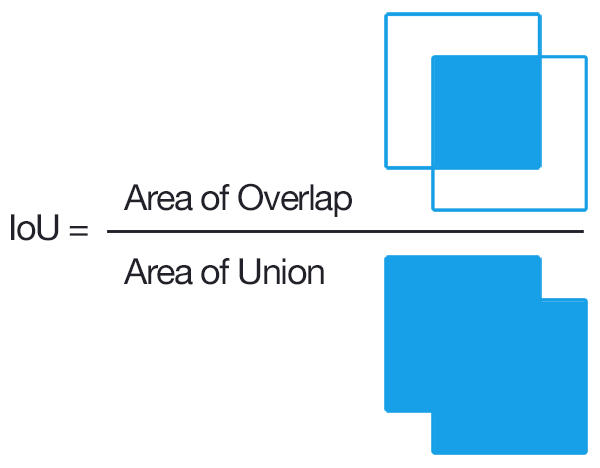
\includegraphics[width=0.8\textwidth]{images/iou_equation.png} %second
				%figure itself
			\end{minipage}
			\caption{Intersection over Union (IoU) as evaluation method for object detection accuracy in a dataset}
			\label{f:iou}
		\end{figure}
	
	
	
\end{enumerate}




\subsection{What problems do they solve}\label{s:ltask}


\begin{figure}[H]
	\begin{center}
		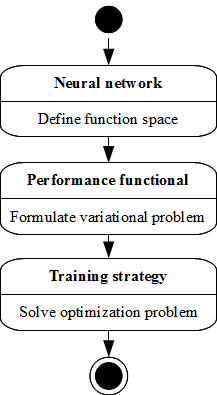
\includegraphics[width=0.35\textwidth]{neural_networks_basis/learning_problem}
		\caption{Learning problem for neural networks.}
		\label{LearningActivityDiagram}
	\end{center}
\end{figure}

Learning tasks for neural networks can be classified according to the source of information for them. \fref{LearningActivityDiagram}

There are basically two sources of information: data sets and mathematical models. 
Some classes of learning tasks which learn from data sets are \emph{function regression}, \emph{pattern recognition} or \emph{time series prediction}. 
Learning tasks in which learning is performed from mathematical models are \emph{optimal control} or \emph{optimal shape design}. 
Finally, in inverse problems the neural network learns from both data sets and mathematical models.



\subsubsection{Function regression}

Function regression is the most popular learning task for neural networks. 
It is also called modelling. The function regression problem can be regarded as the problem of
approximating a function from a data set consisting of input-target instances
\cite{Haykin1994}. The targets are a specification
of what the response to the inputs should be \cite{Bishop1995}. 
While input variables might be quantitative or qualitative, in function regression target variables are quantitative. 

Performance measures for function regression are based on a sum of errors between the outputs from the neural network and the targets in the training data. 
As the training data is usually deficient, a regularization term might be required in order to solve the problem correctly.

An example is to design an instrument that can determine serum cholesterol levels from
measurements of spectral content of a blood sample. There are a number of 
patients for which there are measurements of several wavelengths of the spectrum.
For the same patients there are also measurements of several
cholesterol levels, based on serum separation \cite{Demuth2009}.

Function regression will be used in our problem internally, specifically relative to Bounding-box regression.

% TODO insert bounding-box regression section reference

\subsubsection{Pattern recognition}\label{s:ltask-patt}

The learning task of pattern recognition gives raise to artificial intelligence. That problem can be stated as the process whereby a received pattern, characterized by a distinct
set of features, is assigned to one of a prescribed number of
classes \cite{Haykin1994}. Pattern recognition is also known as classification. Here the neural network learns from knowledge represented by a training data set consisting of input-target instances. The inputs include a set of features which characterize a pattern, and they can be quantitative or qualitative. The targets specify the class that each pattern belongs to and therefore are qualitative \cite{Bishop1995}.

Classification problems can be, in fact, formulated as being modelling problems. 
The learning task of pattern recognition is generally more difficult to solve than that of function regression. 
This means that a good knowledge of the state of the technique is recommended for success. 

A typical example is to disinguish hand-written versions of characters. 
Images of the characters might be captured and fed to a computer. 
We aim to find an algorithm which can distinguish the characters as reliably as possible  \cite{Bishop1995}. 

I'll talk more speficically about pattern recognition problems in \sref{s:patt}, after explaining the basic features of Neural Networks [\sref{s:perc}] and CNNs [\sref{s:cnn-structure}].

\subsubsection{Optimal control}

Optimal control is playing an increasingly important role in the
design of modern engineering systems. The aim
here is the optimization of a physical
process. More specifically, the objective of these problems is to
determine the control signals that will cause a process to satisfy
the physical constraints and at the same time minimize or maximize
some performance criterion \cite{Kirk1970} \cite{BalsaCanto2001}. 

The knowledge in optimal control problems is not represented in the form of a data set, it is given by a mathematical model. 
These objective functionals are often defined by integrals, ordinary differential equations or partial differential equations. 
This way, in order to evaluate them, we might need to apply Simpon methods, Runge-Kutta methods or other finite element methods. 
Optimal control problems often include constraints. 

As a simple example, consider the problem of a rocket launching a
satellite into an orbit around the earth. An associated optimal
control problem is to choose the controls (the thrust attitude angle
and the rate of emission of the exhaust gases) so that the rocket
takes the satellite into its prescribed orbit with minimum
expenditure of fuel or in minimum time.

\subsubsection{Optimal shape design}

Optimal shape design is a very interesting field for industrial
applications. The goal in these problems
is to computerize the development process of some tool, and
therefore shorten the time it takes to create or to improve the
existing one. Being more precise, in an optimal shape design process
one wishes to optimize some performance criterium involving the
solution of a mathematical model with respect to its domain of
definition \cite{Bucur2005}. 

As in the previous case, the neural network here learns from a mathematical model. 
Evaluation of the performance functional here might also need the integration of functions, ordinary differential equations or partial differential equations. 
Optimal shape design problems defined by partial differential equations are challenging applications. 

One example is the design of airfoils,
which proceeds from a knowledge of computational fluid dynamics
\cite{Eyi1994} \cite{Mohammadi2004}. The performance goal here might
vary, but increasing lift and reducing drag are among the most common. Other objectives as weight reduction, stress reinforcement and
even noise reduction can be obtained. On the other hand, the airfoil
may be required to achieve this performance with constraints on
thickness, pitching moment, etc.

\subsubsection{Inverse problems}

Inverse problems can be described as being opposed to direct
problems. In a direct problem the cause is given, and the effect is
determined. In an inverse problem the effect is given, and the cause
is estimated \cite{Kirsch1996} \cite{Sabatier2000} \cite{Ramm2005}.
There are two main types of inverse problems: input estimation, in
which the system properties and output are known and the input is to
be estimated; and properties estimation, in which the the system
input and output are known and the properties are to be estimated.
Inverse problems can be found in many areas of science and
engineering. 

This type of problems is of great interest from both a theoretical and practical perspectives. 
From a theoretical point of view, the neural network here needs both mathematical models and data sets. 
The aim is usually formulated as to find properties or inputs which make a mathematical model to comply with the data set. 
From a practical point of view, most numerical software must be tuned up before being on production. 
That means that the particular properties of a system must be properly estimated in order to simulate it well.

A typical inverse problem in geophysics is to find the 
subsurface inhomogeneities from collected scattered fields caused by
acoustic waves sent at the surface and a mathematical model of soil mechanics.  

\subsubsection{Tasks overview}

The knowledge for a neural network can be represented in the form of data sets or mathematical models. 
The neural network learns from data sets in function regression and pattern recognition; 
it learns from mathematical models in optimal control and optimal shape design; 
and it learns from both mathematical models and data sets in inverse problems. 

\fref{LearningTasksFigure} shows the learning tasks for neural networks described in this section. 
As we can see, they are capable of dealing with a great range of applications. 
Modelling and classification are the most traditional; 
optimal control, optimal shape design and inverse problems can also be very useful.

Our learning task, that \maskrcnn solves really well, is Pattern Recognition (\sref{s:ltask-patt}).

\begin{figure}[H]
	\begin{center}
		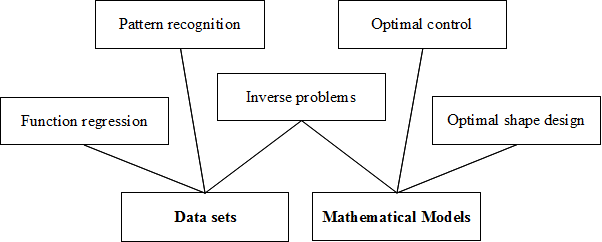
\includegraphics[width=1.0\textwidth]{neural_networks_basis/learning_tasks}
		\caption{Learning tasks for neural networks.}\label{LearningTasksFigure}
	\end{center}
\end{figure}



\subsection{The Perceptron}\label{s:perc}
\begin{figure}[H]
	\centering
	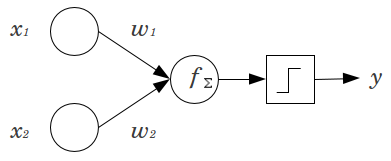
\includegraphics[scale=0.5]{images/2MVdW}
	\caption{The Perceptron}
	\label{f:perceptron}
\end{figure}
\subsubsection{Definition}

A perceptron is the fundamental unit of a Neural Network (which is even called a Multi-Layer Perceptron for this reason). Refer to the diagram above. Perceptrons contain two or more inputs, a weight for each input, a bias, an activation function (the step function) and an output.
For the perceptron above with $2$ inputs, the intermediate value $f(x)$ is as follows
\[f(x) = w_1x_1 + w_2x_2 + b\]
The final output $y$ is just the step function:
\[
y =
\begin{cases}
0 & \text{if $f(x) < 0$} \\
1 & \text{if $f(x) > 0$}
\end{cases}
\]
\subsubsection{Visualization}

The purpose of a perceptron is to classify data. Consider the function AND.

\begin{table}[H]
	\centering
	\begin{tabular}{ |c|c|c| } 
		\hline
		x1 & x2 & out \\
		\hline
		0 & 0 & 0 \\ 
		0 & 1 & 0 \\ 
		1 & 0 & 0 \\ 
		1 & 1 & 1 \\ 
		\hline
	\end{tabular}
	\caption{Function AND}
	\label{t:and}
\end{table}
Let's graph this data.
\begin{center}
	\begin{tikzpicture}
	\begin{axis}[
	axis lines=middle,
	xmin=-1, xmax=2,
	ymin=-1, ymax=2,
	xtick=\empty, ytick=\empty
	]
	\addplot [only marks] table {
		0 0
		0 1
		1 0
	};
	\addplot [only marks, mark=o] table {
		1 1
	};
	\addplot [domain=-10:10, samples=2, dashed] {-1*x+1.5};
	\end{axis}
	\end{tikzpicture}
\end{center}

The line $y = -x + 1.5$ splits this data the best.
Let's rearrange this to get $x + y - 1.5 = 0$. 
Going back to the perceptron formula
\[f(x) = w_1x_1 + w_2x_2 + b\]
we can see that for the optimal perceptron,  $w_1$ and $w_2$ are the coefficients of $x$ and $y$, and $b=-1.5$. If $f(x) > 0$, then $x + y - 1.5>0$. We can see through this example that perceptrons are nothing more than linear functions. Above a line, perceptrons classify data points $1$, below the line, they are $0$.

\subsubsection{Learning}

How do perceptrons "learn" the best possible linear function to split the data? Perceptrons adjust the weights and bias to iteratively approach a solution.

Let's consider this data:
\begin{center}
	\begin{tikzpicture}
	\begin{axis}[
	axis lines=middle,
	xmin=-3, xmax=3,
	ymin=-3, ymax=3,
	xtick=1, ytick=1,
	]
	\addplot [only marks] table {
		0 0
		-1 2 
		1 -2
		-1 -2
		-2 0
	};
	\addplot [only marks, mark=o] table {
		1 1
		0 2
		2 2
		1 3
		1 0
	};
	\addplot [domain=-10:10, samples=2, dashed] {-1*x+1.5};
	\end{axis}
	\end{tikzpicture}
\end{center}

The perceptron that represents the dashed line $y+x-1.5=0$ has two inputs, $x_1, x_2,$ with corresponding weights $w_1=1, w_2=1$, and bias $b = -1.5$. Let $y$ represent the output of this perceptron. In the data above, the point $(1, 0)$ is the only misclassified point. The perceptron outputs 0 because it is below the line, but it should output a 1.

For some data point (input) $i$ with coordinates $(i_1, i_2)$, the perceptron adjusts its weights and bias according to this formula:
\[w_1 = w_1 + \alpha(d-y)(i_1)\]
\[w_2 = w_2 + \alpha(d-y)(i_2)\]
\[b = b + \alpha(d-y)\]
Where $d$ is the desired output, and $\alpha$ is the learning rate, a constant usually between $0$ and $1$. Notice that the equation degenerates to $w = w$ and $b=b$ when the desired output equals the perceptron output. In other words, the perceptron only learns from misclassified points.

In the case of the above data, the perceptron only learns from the point $(1, 0)$. Let's set $\alpha=0.2$ and compute the learning steps:
\[w_1 = 1 + 0.2(1-0)(1) = 1.2\]
\[w_2 = 1 + 0.2(1-0)(0) = 1\]
\[b = -1.5 + 0.2(1-0) = -1.3\]

After 1 iteration, the perceptron now represents the function $y+1.2x-1.3 = 0$, which is shown below:
\begin{center}
	\begin{tikzpicture}
	\begin{axis}[
	axis lines=middle,
	xmin=-3, xmax=3,
	ymin=-3, ymax=3,
	xtick=1, ytick=1,
	]
	\addplot [only marks] table {
		0 0
		-1 2 
		1 -2
		-1 -2
		-2 0
	};
	\addplot [only marks, mark=o] table {
		1 1
		0 2
		2 2
		1 3
		1 0
	};
	\addplot [domain=-10:10, samples=2, dashed] {-1.2*x+1.3};
	\end{axis}
	\end{tikzpicture}
\end{center}

The next iteration follows:
\[w_1 = 1.2 + 0.2(1-0)(1) = 1.4\]
\[w_2 = 1 + 0.2(1-0)(0) = 1\]
\[b = -1.3 + 0.2(1-0) = -1.1\]

\begin{center}
	\begin{tikzpicture}
	\begin{axis}[
	axis lines=middle,
	xmin=-3, xmax=3,
	ymin=-3, ymax=3,
	xtick=1, ytick=1,
	]
	\addplot [only marks] table {
		0 0
		-1 2 
		1 -2
		-1 -2
		-2 0
	};
	\addplot [only marks, mark=o] table {
		1 1
		0 2
		2 2
		1 3
		1 0
	};
	\addplot [domain=-10:10, samples=2, dashed] {-1.4*x+1.1};
	\end{axis}
	\end{tikzpicture}
\end{center}

All the points are now correctly classified. The perceptron has learned! Notice how it has not learned the best possible line, only the first one that zeroes the difference between expected and actual output.
\subsubsection{Non-Linearly Separable Data}
Consider the function XOR:

\begin{table}[H]
	\centering
	\begin{tabular}{ |c|c|c| } 
		\hline
		x1 & x2 & out \\
		\hline
		0 & 0 & 1 \\ 
		0 & 1 & 0 \\ 
		1 & 0 & 0 \\ 
		1 & 1 & 1 \\ 
		\hline
	\end{tabular}
	\caption{Function XOR}
	\label{t:xor}
\end{table}
Let's graph this data.
\begin{center}
	\begin{tikzpicture}
	\begin{axis}[
	axis lines=middle,
	xmin=-1, xmax=2,
	ymin=-1, ymax=2,
	xtick=\empty, ytick=\empty
	]
	\addplot [only marks] table {
		0 1
		1 0
	};
	\addplot [only marks, mark=o] table {
		0 0
		1 1
	};
	\addplot [domain=-10:10, samples=2, dashed] {-1*x+1.5};
	\addplot [domain=-10:10, samples=2, dashed] {-1*x+0.5};
	\end{axis}
	\end{tikzpicture}
\end{center}

We need two lines to separate this data! A perceptron will never reach the optimal solution. However, multiple perceptrons can learn multiple lines, which can be used to classify non-linearly separable data.

\subsubsection{Multi-Layer Perceptron}
A neural network (NN) or Multi-Layer Perceptron (MLP) is a bunch of these perceptrons glued together, and can be used to approximate multi-dimensional non-linearly separable data.
Let's again consider XOR. How do we arrange perceptrons to represent the two functions?

Clearly, we need two perceptrons, one for each function. The output of these two perceptrons can be used as inputs to a third perceptron, which will give us our output. Refer to the diagram below.

\begin{figure}[H]
	\centering
	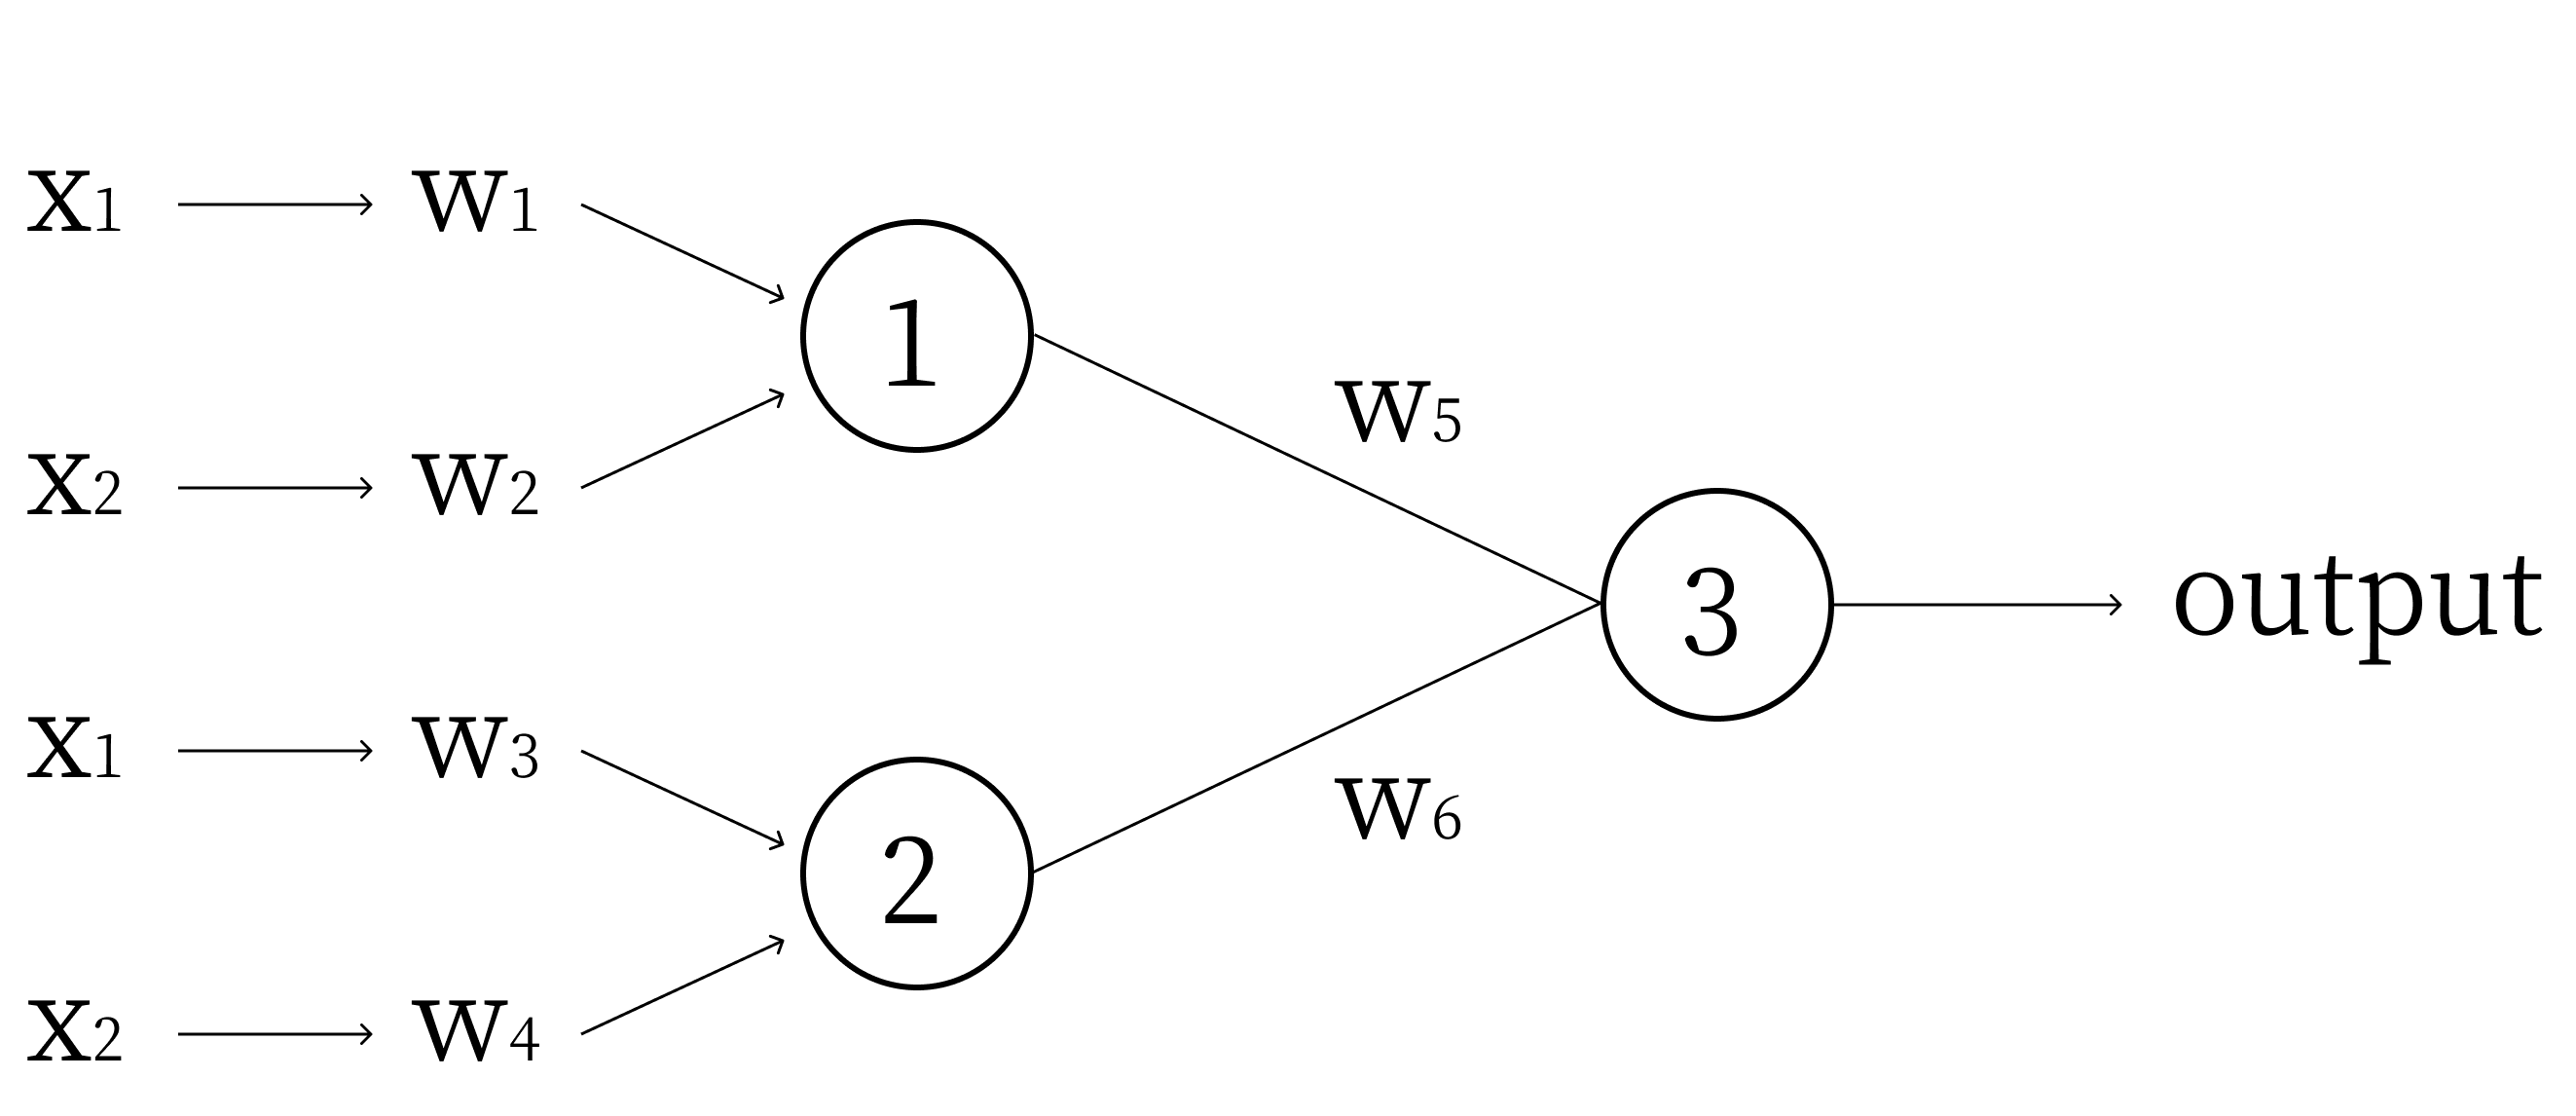
\includegraphics[scale=0.3]{images/Frame}
	\caption{Multi-Layer Perceptron}
	\label{f:Frame}
\end{figure}

Let perceptron 1 model $y + x - 1.5 = 0$ (the upper line), and perceptron 2 model $y + x - 0.5 = 0$ (the lower line). Because the weights are the coefficients of these functions, $w_1 = 1, w_2 = 1, w_3 = 1, w_4 = 1$ and the biases $b_1 = -1.5$ and $b_2 = -0.5$.

The output of Perceptron 1 will be a 1 for points above the upper line, and a 0 for the points below the upper line. The output of Perceptron 2 will be a 1 for points above the lower line, and a 0 for points below the lower line. In between the lines, these cancel! However, in order to create a threshold to separate the points between the lines from the points outside, we would like the outputs for points between the lines to be additive.

In other words, we would like the inputs of Perceptron 3 to both be 1 between the lines, and have a maximum of a single 1 for points outside the lines. Thus, we let $w_6 = 1$ and $w_5 = -1$. This gives us an output of $2$ for points between the lines, and a maximum output of 1 for points outside the lines. Thus, we can set the bias for Perceptron 3: $b_3 = -1.5$.


% ------------------------------------------------------------------
\subsection{Convolutional Neural Network}\label{s:cnn-structure}
% ------------------------------------------------------------------

A \emph{Neural Network} (NN) is a function $g$ mapping data $\bx$, for example an image, to an output vector $\by$, for example an image label. The function $g=f_L \circ \dots \circ f_1$ is the composition of a sequence of simpler functions $f_l$, which are called \emph{computational blocks} [\sref{s:blocks}] or \emph{layers}. Let $\bx_1,\bx_2,\dots,\bx_L$ be the outputs of each layer in the network, and let $\bx_0=\bx$ denote the network input. Each intermediate output $\bx_l = f_l(\bx_{l-1};\bw_l)$ is computed from the previous output $\bx_{l-1}$  by applying the function $f_l$ with parameters $\bw_l$. 

In a \emph{Convolutional Neural Network} (CNN), the data has a spatial structure: each $\bx_l\in\mathbb{R}^{H_l \times W_l \times C_l}$ is a 3D array or \emph{tensor} where the first two dimensions $H_l$ (height) and $W_l$ (width) are interpreted as spatial dimensions. The third dimension $C_l$ is instead interpreted as the \emph{number of feature channels}. Hence, the tensor $\bx_l$ represents a $H_l \times W_l$ field of $C_l$-dimensional feature vectors, one for each spatial location. A fourth dimension $N_l$ in the tensor spans multiple data samples packed in a single \emph{batch} for efficiency parallel processing. The number of data samples $N_l$ in a batch is called the batch \emph{cardinality}. The network is called \emph{convolutional} because the functions $f_l$ are local and translation invariant operators (i.e.\ non-linear filters) like linear convolution.

It is also possible to conceive CNNs with more than two spatial dimensions, where the additional dimensions may represent volume or time. In fact, there are little \emph{a-priori} restrictions on the format of data in neural networks in general. Many useful NNs contain a mixture of convolutional layers together with layer that process other data types such as text strings, or perform other operations that do not strictly conform  to the CNN assumptions.

There are a variety of layers such as (convolution),  (convolution transpose or deconvolution),  (max and average pooling),  (ReLU activation),  (sigmoid activation),  (softmax operator),  (classification log-loss), (batch normalization), (spatial normalization), (local response normalization -- LRN). 

NNs are often used as classifiers or regressors. In the example of \sref{f:demo}, the output $\hat \by = f(\bx)$ is a vector of probabilities, one for each of a 1,000 possible image labels (dog, cat, trilobite, ...).  If $\by$ is the true label of image $\bx$, we can measure the CNN performance by a loss function $\ell_\by(\hat \by)  \in \mathbb{R}$ which assigns a penalty to classification errors. The CNN parameters can then be tuned or \emph{learned} to minimize this loss averaged over a large dataset of labelled example images.

% ------------------------------------------------------------------
\subsubsection{Optimizers}\label{s:cnn-optimizers}
% ------------------------------------------------------------------

Learning generally uses a variant of \emph{stochastic gradient descent} (SGD). While this is an efficient method (for this type of problems), networks may contain several million parameters and need to be trained on millions of images. SGD also requires to compute the CNN derivatives, as explained in the next section. Our \maskrcnn uses Adam as optimizer, not SGD, although SGD seems to have better segmentation performance, albeit a bit slower to learn \cite{wilson2017marginal}.
\begin{quotation}“We observe that the solutions found by adaptive methods generalize worse (often significantly worse) than SGD, even when these solutions have better training performance. These results suggest that practitioners should reconsider the use of adaptive methods to train neural networks."
\end{quotation}

\begin{figure}[H]
	\centering
	\includegraphics[width=0.5\columnwidth]{figures/pepper}
	\caption{An example of one of  \matlab stock images using a large CNN pre-trained on ImageNet.}
	\label{f:demo}
\end{figure}

% ------------------------------------------------------------------
\subsubsection{Network structures}\label{s:cnn-topology}
% ------------------------------------------------------------------

In the simplest case, layers in a NN are arranged in a sequence; however, more complex interconnections are possible as well, and in fact very useful in many cases. This section discusses such configurations and introduces a graphical notation to visualize them.

% ------------------------------------------------------------------
\paragraph{Sequences}\label{s:cnn-simple}
% ------------------------------------------------------------------

Start by considering a computational block $f$ in the network. This can be represented schematically as a box receiving data $\bx$ and parameters $\bw$ as inputs and producing data $\by$ as output:
\begin{center}
	\begin{tikzpicture}[auto, node distance=2cm]
	\node (x) [data] {$\bx$};
	\node (f) [block,right of=x]{$f$};
	\node (y) [data, right of=f] {$\by$};
	\node (w) [data, below of=f] {$\bw$};
	\draw [to] (x.east) -- (f.west) {};
	\draw [to] (f.east) -- (y.west) {};
	\draw [to] (w.north) -- (f.south) {};
	\end{tikzpicture}
\end{center}
As seen above, in the simplest case blocks are chained in a sequence $f_1 \rightarrow f_2\rightarrow\dots\rightarrow f_L$ yielding the structure:
\begin{center}
	\begin{tikzpicture}[auto, node distance=2cm]
	\node (x0)  [data] {$\bx_0$};
	\node (f1) [block,right of=x0]{$f_1$};
	\node (f2) [block,right of=f1,node distance=3cm]{$f_2$};
	\node (dots) [right of=f2]{...};
	\node (fL) [block,right of=dots]{$f_L$};
	\node (xL)  [data, right of=fL] {$\bx_L$};
	\node (w1) [data, below of=f1] {$\bw_1$};
	\node (w2) [data, below of=f2] {$\bw_2$};
	\node (wL) [data, below of=fL] {$\bw_L$};
	\draw [to] (x0.east) -- (f1.west) {};
	\draw [to] (f1.east) -- node {$\bx_1$} (f2.west);
	\draw [to] (f2.east) -- node {$\bx_2$} (dots.west) {};
	\draw [to] (dots.east) -- node {$\bx_{L-1}$} (fL.west) {};
	\draw [to] (fL.east) -- (xL.west) {};
	\draw [to] (w1.north) -- (f1.south) {};
	\draw [to] (w2.north) -- (f2.south) {};
	\draw [to] (wL.north) -- (fL.south) {};
	\end{tikzpicture}
\end{center}
Given an input $\bx_0$, evaluating the network is a simple matter of evaluating all the blocks from left to right, which defines a composite function $\bx_L = f(\bx_0;\bw_1,\dots,\bw_L)$. 

% ------------------------------------------------------------------
\paragraph{Directed acyclic graphs}\label{s:cnn-dag}
% ------------------------------------------------------------------

\begin{figure}[t]
	\begin{center}
		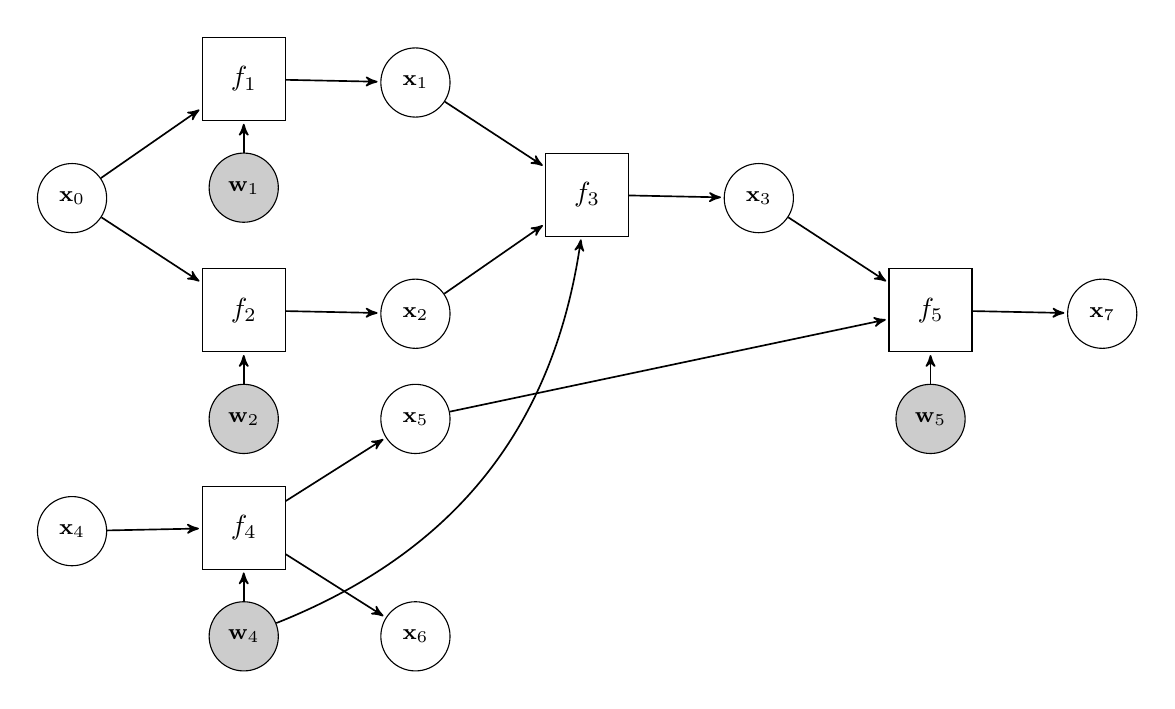
\begin{tikzpicture}[auto, node distance=0.4cm]
		\matrix (m) [matrix of math nodes, 
		column sep=1.2cm,
		row sep=0.4cm]
		{
			& \node (f1) [block]{f_1}; 
			& \node (x1) [datac]{\bx_1};
			\\
			\node (x0) [datac]{\bx_0};
			&
			&
			& \node (f3) [block]{f_3};
			& \node (x3) [datac]{\bx_3};
			\\
			& \node (f2) [block]{f_2}; 
			& \node (x2) [datac]{\bx_2};
			& &
			& \node (f5) [block]{f_5}; 
			& \node (x7) [datac]{\bx_7}; 
			\\
			& 
			& \node(x5) [datac]{\bx_5};
			\\
			\node (x4) [datac]{\bx_4};
			& \node (f4) [block]{f_4};
			\\
			& 
			& \node(x6) [datac]{\bx_6};
			\\
		};
		\draw[to] (x0) -- (f1);
		\draw[to] (f1) -- (x1);
		\draw[to] (x1) -- (f3);
		\draw[to] (x0) -- (f2);
		\draw[to] (f2) -- (x2);
		\draw[to] (x2) -- (f3);
		\draw[to] (f3) -- (x3);
		\draw[to] (x3) -- (f5);
		\draw[to] (f5) -- (x7);
		\draw[to] (x4) -- (f4);
		\draw[to] (f4) -- (x5);
		\draw[to] (f4) -- (x6);
		\draw[to] (x5) -- (f5);
		\node(w1) [par,below=of f1]{$\bw_1$}; \draw[to] (w1) -- (f1);
		\node(w2) [par,below=of f2]{$\bw_2$}; \draw[to] (w2) -- (f2);
		%\node(w3) [par,below=of f3]{$\bw_3$}; \draw[to] (w3) -- (f3);
		\node(w4) [par,below=of f4]{$\bw_4$}; \draw[to] (w4) -- (f4);
		\draw[to] (w4) to [bend right] (f3);
		\node(w5) [par,below=of f5]{$\bw_5$}; \draw[to] (w5) -- (f5);
		\end{tikzpicture}
	\end{center}
	\vspace{-1em}
	\caption{\textbf{Example DAG.}}\label{f:dag}
\end{figure}

One is not limited to chaining layers one after another. In fact, the only requirement for evaluating a NN is that, when a layer has to be evaluated, all its input have been evaluated prior to it. This is possible exactly when the interconnections between layers form a \emph{directed acyclic graph}, or DAG for short.

In order to visualize DAGs, it is useful to introduce additional nodes for the network variables, as in the  example of \fref{f:dag}. Here boxes denote functions and circles denote variables (parameters are treated as a special kind of variables). In the example, $\bx_0$ and $\bx_4$ are the inputs of the CNN and $\bx_6$ and $\bx_7$ the outputs. Functions can take any number of inputs (e.g. $f_3$ and $f_5$ take two) and have any number of outputs (e.g. $f_4$ has two). There are a few noteworthy properties of this graph:

\begin{enumerate}
	\item The graph is bipartite, in the sense that arrows always go from boxes to circles and from circles to boxes. 
	\item Functions can have any number of inputs or outputs; variables and parameters can have an arbitrary number of outputs (a parameter with more of one output is \emph{shared} between different layers); variables have at most one input and parameters none. 
	\item Variables with no incoming arrows and parameters are not computed by the network, but must be set prior to evaluation, i.e.\ they are \emph{inputs}. Any variable (or even parameter) may be used as output, although these are usually the variables with no outgoing arrows.
	\item Since the graph is acyclic, the CNN can be evaluated by sorting the functions and computing them one after another (in the example, evaluating the functions in the order $f_1,f_2,f_3,f_4,f_5$ would work).
\end{enumerate}

% ------------------------------------------------------------------
\subsubsection{Computing derivatives with backpropagation}\label{s:back}
% ------------------------------------------------------------------

Learning a NN requires computing the derivative of the loss with respect to the network parameters. Derivatives are computed using an algorithm called \emph{backpropagation}, which is a memory-efficient implementation of the chain rule for derivatives. First, we discuss the derivatives of a single layer, and then of a whole network.

\paragraph{Derivatives of tensor functions}

In a CNN, a layer is a function $\by = f(\bx)$ where both input $\bx \in \mathbb{R}^{H\times W \times C}$ and output $\by \in \mathbb{R}^{H'\times W' \times C'}$ are tensors. The derivative of the function $f$ contains the derivative of each output component $y_{i'j'k'}$ with respect to each input component $x_{ijk}$, for a total of $H'\times W'\times C'\times H\times W\times C$ elements naturally arranged in a 6D tensor. Instead of expressing derivatives as tensors, it is often useful  to switch to a matrix notation by \emph{stacking} the input and output tensors into vectors. This is done by the $\vv$ operator, which visits each element of a tensor in lexicographical order and produces a vector:
\[
\vv \bx
=
\begin{bmatrix}
x_{111} \\
x_{211} \\
\vdots
\\
x_{H11} \\
x_{121} \\
\vdots \\
x_{HWC}  	
\end{bmatrix}.
\]
By stacking both input and output, each layer $f$ can be seen reinterpreted as vector function $\vv f$, whose derivative is the conventional Jacobian matrix:
\[
\renewcommand*{\arraystretch}{1.5}
\frac{d \vv f}{d(\vv \bx)^\top}
=
\begin{bmatrix}
\frac{\partial y_{111}}{\partial x_{111}} & 
\frac{\partial y_{111}}{\partial x_{211}} &
\dots &
\frac{\partial y_{111}}{\partial x_{H11}} &
\frac{\partial y_{111}}{\partial x_{121}} &
\dots &
\frac{\partial y_{111}}{\partial x_{HWC}} \\
\frac{\partial y_{211}}{\partial x_{111}} & 
\frac{\partial y_{211}}{\partial x_{211}} &
\dots &
\frac{\partial y_{211}}{\partial x_{H11}} &
\frac{\partial y_{211}}{\partial x_{121}} &
\dots &
\frac{\partial y_{211}}{\partial x_{HWC}} \\
\vdots & \vdots & \dots & \vdots & \vdots & \dots & \vdots \\
\frac{\partial y_{H'11}}{\partial x_{111}} & 
\frac{\partial y_{H'11}}{\partial x_{211}} &
\dots &
\frac{\partial y_{H'11}}{\partial x_{H11}} &
\frac{\partial y_{H'11}}{\partial x_{121}} &
\dots &
\frac{\partial y_{H'11}}{\partial x_{HWC}} \\
\frac{\partial y_{121}}{\partial x_{111}} & 
\frac{\partial y_{121}}{\partial x_{211}} &
\dots &
\frac{\partial y_{121}}{\partial x_{H11}} &
\frac{\partial y_{121}}{\partial x_{121}} &
\dots &
\frac{\partial y_{121}}{\partial x_{HWC}} \\
\vdots & \vdots & \dots & \vdots & \vdots & \dots & \vdots \\
\frac{\partial y_{H'W'C'}}{\partial x_{111}} & 
\frac{\partial y_{H'W'C'}}{\partial x_{211}} &
\dots &
\frac{\partial y_{H'W'C'}}{\partial x_{H11}} &
\frac{\partial y_{H'W'C'}}{\partial x_{121}} &
\dots &
\frac{\partial y_{H'W'C'}}{\partial x_{HWC}}
\end{bmatrix}.
\]
This notation for the derivatives of tensor functions is taken from~\cite{kinghorn96integrals} and is used throughout this section.

While it is easy to express the derivatives of tensor functions as matrices, these matrices are in general extremely large. Even for moderate data sizes (e.g. $H=H'=W=W'=32$ and $C=C'=128$), there are $H'W'C'HWC \approx 17 \times 10^9$ elements in the Jacobian. Storing that requires 68 GB of space in single precision. The purpose of the backpropagation algorithm is to compute the derivatives required for learning without incurring this huge memory cost.

\paragraph{Derivatives of function compositions}

In order to understand backpropagation, consider first a simple CNN terminating in a loss function $f_L = \ell_\by$:
\begin{center}
	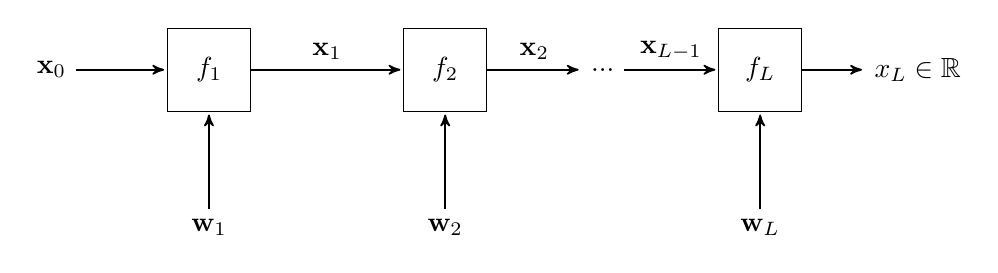
\begin{tikzpicture}[auto, node distance=2cm]
	\node (x0)  [data] {$\bx_0$};
	\node (f1) [block,right of=x0]{$f_1$};
	\node (f2) [block,right of=f1,node distance=3cm]{$f_2$};
	\node (dots) [right of=f2]{...};
	\node (fL) [block,right of=dots]{$f_L$};
	\node (w1) [data, below of=f1] {$\bw_1$};
	\node (w2) [data, below of=f2] {$\bw_2$};
	\node (wL) [data, below of=fL] {$\bw_L$};
	\node (xL) [data, right of=fL] {$x_L\in\real$};
	\draw [to] (x0.east) -- (f1.west) {};
	\draw [to] (f1.east) -- node {$\bx_1$} (f2.west);
	\draw [to] (f2.east) -- node {$\bx_2$} (dots.west) {};
	\draw [to] (dots.east) -- node {$\bx_{L-1}$} (fL.west) {};
	\draw [to] (fL.east) -- (xL.west) {};
	\draw [to] (w1.north) -- (f1.south) {};
	\draw [to] (w2.north) -- (f2.south) {};
	\draw [to] (wL.north) -- (fL.south) {};
	\end{tikzpicture}
\end{center}
The goal is to compute the gradient of the loss value $x_L$ (output) with respect to each network parameter $\bw_l$:
\[
\frac{df}{d(\vv \bw_l)^\top} = 
\frac{d}{d(\vv \bw_l)^\top}
\left[f_L(\cdot;\bw_L) \circ ... \circ 
f_2(\cdot;\bw_2) \circ f_1(\bx_0;\bw_1)\right].
\]
By applying the chain rule and by using the matrix notation introduced above, the derivative can be written as
\begin{equation}\label{e:chain-rule}
\frac{df}{d(\vv \bw_l)^\top} 
= 
\frac{d\vv f_L(\bx_{L-1};\bw_{L})}{d(\vv\bx_{L-1})^\top}
\times
\dots
\times
\frac{d\vv f_{l+1}(\bx_{l};\bw_{l+1})}{d(\vv\bx_{l})^\top}
\times
\frac{d\vv f_l(\bx_{l-1};\bw_{l})}{d(\vv\bw_l^\top)}
\end{equation}
where the derivatives are computed at the working point determined by the input $\bx_0$ and the current value of the parameters. 

Note that, since the network output $x_L$ is a \emph{scalar} quantity, the target derivative $df/d(\vv \bw_l)^\top$ has the same number of elements of the parameter vector $\bw_l$, which is moderate. However, the intermediate Jacobian factors have, as seen above, an unmanageable size. In order to avoid computing these factor explicitly, we can proceed as follows.

Start by multiplying the output of the last layer by a tensor $p_L=1$ (note that this tensor is a scalar just like the variable $x_L$):
\begin{align*}
p_L \times \frac{df}{d(\vv \bw_l)^\top} 
&= 
\underbrace{p_L \times \frac{d\vv f_L(\bx_{L-1};\bw_{L})}{d(\vv\bx_{L-1})^\top}}_{(\vv \bp_{L-1})^\top}
\times
\dots
\times
\frac{d\vv f_{l+1}(\bx_{l};\bw_{l+1})}{d(\vv\bx_{l})^\top}
\times
\frac{d\vv f_l(\bx_{l-1};\bw_{l})}{d(\vv\bw_l^\top)}
\\
&=
(\vv \bp_{L-1})^\top
\times
\dots
\times
\frac{d\vv f_{l+1}(\bx_{l};\bw_{l+1})}{d(\vv\bx_{l})^\top}
\times
\frac{d\vv f_l(\bx_{l-1};\bw_{l})}{d(\vv\bw_l^\top)}
\end{align*}
In the second line the last two factors to the left have been multiplied obtaining a new tensor $\bp_{L-1}$ that has the same size as the variable $\bx_{L-1}$. The factor $\bp_{L-1}$ can therefore be explicitly stored. The construction is then repeated by multiplying pairs of factors from left to right, obtaining a sequence of tensors $\bp_{L-2},\dots,\bp_{l}$ until the desired derivative is obtained. Note that, in doing so, no large tensor is ever stored in memory. This process is known as \emph{backpropagation}.

In general, tensor $\bp_{l}$ is obtained from $\bp_{l+1}$ as the product:
\[
(\vv \bp_{l})^\top = (\vv \bp_{l+1})^\top \times \frac{d\vv f_{l+1}(\bx_{l};\bw_{l+1})}{d(\vv\bx_{l})^\top}.
\]
The key to implement backpropagation is to be able to compute these products without explicitly computing and storing in memory the second factor, which is a large Jacobian matrix. Since computing the derivative is a linear operation, this product can be interpreted as the \emph{derivative of the layer projected along direction $\bp_{l+1}$}: 
\begin{equation}\label{e:projected}
\bp_{l} = 
\frac{d \langle \bp_{l+1}, f(\bx_l;\bw_l) \rangle}
{d \bx_{l}}.
\end{equation}
Here $\langle \cdot,\cdot \rangle$ denotes the inner product between tensors, which results in a scalar quantity. Hence the derivative \eqref{e:projected} needs not to use the $\vv$ notation, and yields a tensor $\bp_l$ that has the same size as $\bx_l$ as expected.

In order to implement backpropagation, the CNN for each layer $f$ can have:
\begin{itemize}
	\item A \textbf{forward mode}, computing the output $\by = f(\bx;\bw)$ of the layer given its input $\bx$ and parameters $\bw$.
	\item A \textbf{backward mode}, computing the projected derivatives
	\[
	\frac{d \langle \bp, f(\bx;\bw) \rangle}
	{d \bx}
	\quad\text{and}\quad
	\frac{d \langle \bp, f(\bx;\bw) \rangle}
	{d \bw},
	\]
	given, in addition to the input $\bx$ and parameters $\bw$, a tensor $\bp$ that the same size as $\by$.
\end{itemize}
%This is best illustrated with an example. Consider a layer $f$ such as the convolution operator. In the ``forward'' mode, one calls the function as $y = vl_nnconv(x,w,[])$ to apply the filters $w$ to the input $x$ and obtain the output $y$. In the ``backward mode'', one calls $[dx, dw] = vl_nnconv(x,w,[],p)$.  As explained above, $dx$, $dw$, and $p$ have the same size as $x$, $w$, and $y$, respectively. The computation of large Jacobian is encapsulated in the function call and never carried out explicitly. 

% TODO training algorithm with mention to overfitting

\paragraph{Backpropagation networks}\label{s:bpnets}

In this section, we provide a schematic interpretation of backpropagation and show how it can be implemented by ``reversing'' the NN computational graph.

The projected derivative of eq.~\eqref{e:projected} can be seen as the derivative of the following mini-network:
\begin{center}
	\begin{tikzpicture}[auto, node distance=2cm]
	\node (x) [data] {$\bx$};
	\node (f) [block,right of=x ] {$f$};
	\node (dot)[block,right of=f ] {$\langle \cdot, \cdot \rangle$};
	\node (z) [data, right of=dot] {$z \in \mathbb{R}$};
	\node (w) [data, below of=f ] {$\bw$};
	\node (p) [data, below of=dot] {$\bp$};
	\draw [to] (x.east) -- (f.west) {};
	\draw [to] (f.east) -- node {$\by$}  (dot.west) {};
	\draw [to] (w.north) -- (f.south) {};
	\draw [to] (dot.east) -- (z.west) {};
	\draw [to] (p.north) -- (dot.south) {};
	\end{tikzpicture}
\end{center}
In the context of back-propagation, it can be useful to think of the projection $\bp$ as the ``linearization'' of the rest of the network from variable $\by$ down to the loss. The projected derivative can also be though of as a new layer $(d\bx, d\bw) = df(\bx,\bw,\bp)$ that, by computing the derivative of the mini-network, operates in the reverse direction:
\begin{center}
	\begin{tikzpicture}[auto, node distance=2cm]
	\node (df) [block,right of=x] {$df$};
	\node (dx) [data,left of=df] {$d\bx$};
	\node (dw) [data,below of=df] {$d\bw$};
	\node (w) [data,above of=df,xshift=0.6em] {$\bw$};
	\node (x) [data,above of=df,xshift=-0.6em] {$\bx$};
	\node (p) [data,right of=df] {$\bp$};
	\draw [to] (df.west) -- (dx.east)  {};
	\draw [to] (df.south) -- (dw.north)  {};
	\draw [to] (p.west) -- (f.east) {};
	\draw [to] (w.south) -- ([xshift=0.6em]df.north) {};
	\draw [to] (x.south) -- ([xshift=-0.6em]df.north) {};
	\end{tikzpicture}
\end{center}
By construction (see eq.~\eqref{e:projected}), the function $df$ is \emph{linear} in the argument $\bp$.

Using this notation, the forward and backward passes through the original network can be rewritten as evaluating an extended network which contains a BP-reverse of the original one (in blue in the diagram):
\begin{center}
	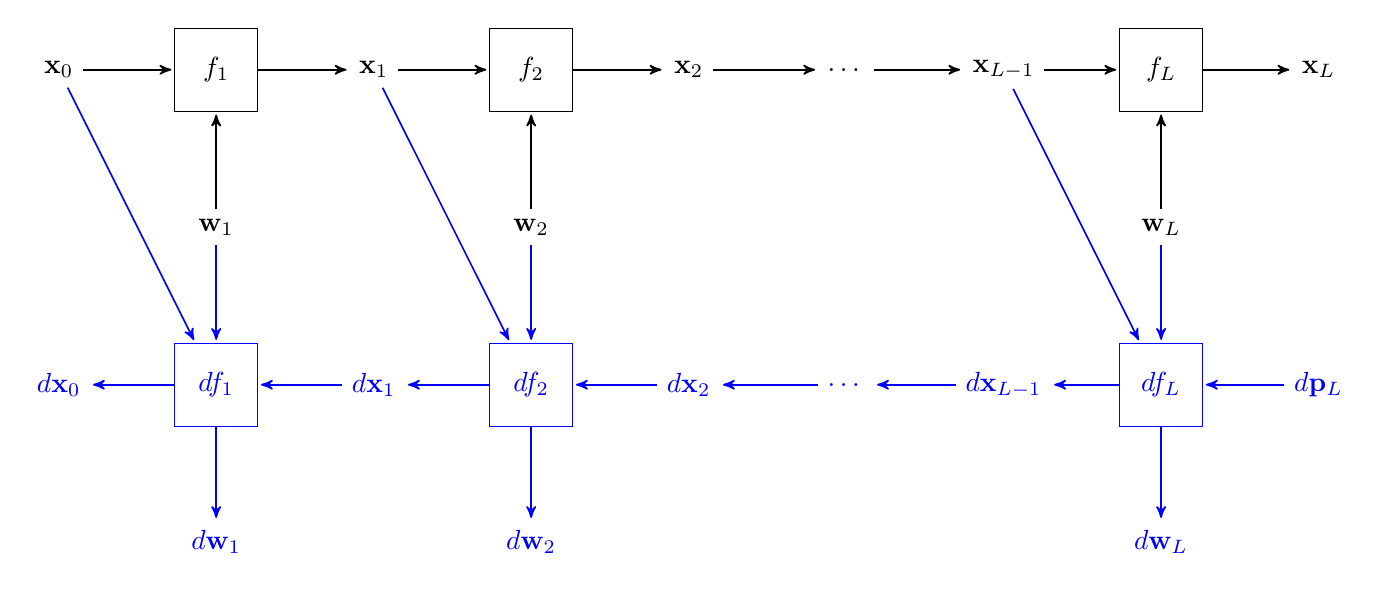
\begin{tikzpicture}[auto, node distance=2cm]
	\node (x0) [data] {$\bx_0$};
	%
	\node (f1) [block,right of=x0] {$f_1$};
	\node (x1) [data,right of=f1] {$\bx_{1}$};
	\node (w1) [data,below of=f1] {$\bw_1$};
	%
	\node (f2) [block,right of=x1] {$f_2$};
	\node (x2) [data,right of=f2] {$\bx_{2}$};
	\node (w2) [data,below of=f2] {$\bw_2$};
	%
	\node (f3) [right of=x2] {$\dots$};
	\node (xLm) [right of=f3] {$\bx_{L-1}$};
	%
	\node (fL) [block,right of=xLm] {$f_L$};
	\node (xL) [data,right of=fL] {$\bx_{L}$};
	\node (wL) [data,below of=fL] {$\bw_L$};
	%
	\draw [to] (x0.east) -- (f1.west) {};
	%
	\draw [to] (w1.north) -- (f1.south) {};
	\draw [to] (f1.east) -- (x1.west) {};
	\draw [to] (x1.east) -- (f2.west) {};
	%
	\draw [to] (w2.north) -- (f2.south) {};
	\draw [to] (f2.east) -- (x2.west) {};
	\draw [to] (x2.east) -- (f3.west) {};
	%
	\draw [to] (f3.east) -- (xLm.west) {};
	\draw [to] (xLm.east) -- (fL.west) {};
	%
	\draw [to] (wL.north) -- (fL.south) {};
	\draw [to] (fL.east) -- (xL.west) {};
	%
	\node (dfL) [block,below of=wL,bp] {$df_L$};
	\node (dxL) [data,right of=dfL,bpe] {$d\bp_L$};
	\node (dwL) [data,below of=dfL,bpe] {$d\bw_L$};
	\node (dxLm) [data,left of=dfL,bpe] {$d\bx_{L-1}$};
	%
	\node (df3) [left of=dxLm,bpe] {$\dots$};
	%
	\node (df2) [block,below of=w2,bp] {$df_2$};
	\node (dx2) [data,right of=df2,bpe] {$d\bx_{2}$};
	\node (dw2) [data,below of=df2,bpe] {$d\bw_2$};
	%
	\node (df1) [block,below of=w1,bp] {$df_1$};
	\node (dx1) [data,right of=df1,bpe] {$d\bx_{1}$};
	\node (dw1) [data,below of=df1,bpe] {$d\bw_1$};
	%
	\node (dx0) [data,left of=df1,bpe] {$d\bx_{0}$};
	%
	\draw [to,bp] (wL.south) -- (dfL.north) {};
	\draw [to,bp] (dfL.south) -- (dwL.north) {};
	\draw [to,bp] (dxL.west) -- (dfL.east) {};
	\draw [to,bp] (dfL.west) -- (dxLm.east) {};
	%
	\draw [to,bp] (dxLm.west) -- (df3.east) {};
	\draw [to,bp] (df3.west) -- (dx2.east) {};
	%
	\draw [to,bp] (w2.south) -- (df2.north) {};
	\draw [to,bp] (df2.south) -- (dw2.north) {};
	\draw [to,bp] (dx2.west) -- (df2.east) {};
	\draw [to,bp] (df2.west) -- (dx1.east) {};
	%
	\draw [to,bp] (w1.south) -- (df1.north) {};
	\draw [to,bp] (df1.south) -- (dw1.north) {};
	\draw [to,bp] (dx1.west) -- (df1.east) {};
	%
	\draw [to,bp] (df1.west) -- (dx0.east) {};
	%
	\draw [to,bp] (x0) -- (df1) {} ;
	\draw [to,bp] (x1) -- (df2) {} ;
	\draw [to,bp] (xLm) -- (dfL) {} ;
	\end{tikzpicture}
\end{center}

% ------------------------------------------------------------------
\paragraph{Backpropagation in DAGs}\label{s:dag}
% ------------------------------------------------------------------

Assume that the DAG has a single output variable $\bx_L$ and assume, without loss of generality, that all variables are sorted in order of computation $(\bx_0,\bx_1,\dots,\bx_{L-1},\bx_L)$ according to the DAG structure. Furthermore, in order to simplify the notation, assume that this list contains both data and parameter variables, as the distinction is moot for the discussion in this section.

We can cut the DAG at any point in the sequence by fixing $\bx_0, \dots, \bx_{l-1}$ to some arbitrary value and dropping all the DAG layers that feed into them, effectively transforming the first $l$ variables into inputs. Then, the rest of the DAG defines a function $h_l$ that maps these input variables to the output $\bx_L$:
\[
\bx_L = h_l(\bx_0,\bx_1,\dots,\bx_{l-1}).
\]
Next, we show that backpropagation in a DAG iteratively computes the projected derivatives of all functions $h_1,\dots,h_L$ with respect to all their parameters.

Backpropagation starts by initializing variables $(d\bx_{0},\dots,d\bx_{l-1})$ to null tensors of the same size as $(\bx_0,\dots,\bx_{l-1})$. Next, it computes the projected derivatives of
\[
\bx_L = h_L(\bx_0,\bx_1,\dots,\bx_{L-1}) =
f_{\pi_L}(\bx_0,\bx_1,\dots,\bx_{L-1}).
\]
Here $\pi_l$ denotes the index of the layer $f_{\pi_l}$ that computes the value of the variable $\bx_l$. There is at most one such layer, or none if $\bx_l$ is an input or parameter of the original NN. In the first case, the layer may depend on any of the variables prior to $\bx_l$ in the sequence, so that general one has:
\[
\bx_{l} = f_{\pi_l}(\bx_0,\dots,\bx_{l-1}).
\]
At the beginning of backpropagation, since there are no intermediate variables between $\bx_{L-1}$ and $\bx_L$, the function $h_L$ is the same as the last layer $f_{\pi_L}$. Thus the projected derivatives of $h_L$ are the same as the projected derivatives of $f_{\pi_L}$, resulting in the equation
\[
\forall t=0,\dots,L-1:\qquad
d\bx_{t} \leftarrow d\bx_{t}
+ \frac{d\langle \bp_L, f_{\pi_L}(\bx_0,\dots,\bx_{t-1})\rangle}{d\bx_t}.
\]
Here, for uniformity with the other iterations, we use the fact that $d\bx_l$ are initialized to zero and \emph{accumulate} the values instead of storing them. In practice, the update operation needs to be carried out only for the variables $\bx_l$ that are actual inputs to $f_{\pi_L}$, which is often a tiny fraction of all the variables in the DAG.

After the update, each $d\bx_t$ contains the projected derivative of function $h_L$ with respect to the corresponding variable:
\[
\forall t=0,\dots,L-1:\qquad
d\bx_t = \frac{d\langle \bp_L, h_L(\bx_0,\dots,\bx_{l-1})\rangle}{d\bx_t}.
\]
Given this information, the next iteration of backpropagation updates the variables to contain the projected derivatives of $h_{L-1}$ instead. In general, given the derivatives of $h_{l+1}$, backpropagation computes the derivatives of $h_{l}$ by using the relation
\[
\bx_L
= 
h_{l}(\bx_0,\bx_1,\dots,\bx_{l-1})
=
h_{l+1}(\bx_0,\bx_1,\dots,\bx_{l-1},f_{\pi_L}(\bx_0,\dots,\bx_{l-1}))
\]
Applying the chain rule to this expression, for all $0\leq t \leq l-1$:
\[
\frac{d\langle \bp, h_l \rangle}{d(\vv \bx_t)^\top}
=
\frac{d\langle \bp, h_{l+1}\rangle}{d(\vv \bx_t)^\top}
+
\underbrace{\frac{d\langle \bp_L, h_{l+1}\rangle}{d(\vv \bx_l)^\top}}_{\vv d\bx_l}
\frac{d \vv f_{\pi_l}}{d(\vv \bx_t)^\top}.
\]
This yields the update equation
\begin{equation}\label{e:bp-update}	
\forall t=0,\dots,l-1:\qquad
d\bx_t \leftarrow d\bx_t + \frac{d\langle \bp_l, f_{\pi_l}(\bx_0,\dots,\bx_{l-1})\rangle}{d\bx_t},
\quad
\text{where\ }
\bp_l = d\bx_l.
\end{equation}
Once more, the update needs to be explicitly carried out only for the variables $\bx_t$ that are actual inputs of $f_{\pi_l}$. In particular, if $\bx_l$ is a data input or a parameter of the original neural network, then $\bx_l$ does not depend on any other variables or parameters and $f_{\pi_l}$ is a nullary function (i.e.\ a function with no arguments). In this case, the update does not do anything. 
After iteration $L-l+1$ completes, backpropagation remains with:
\begin{align*}
\forall t=0,\dots,l-1:&\qquad
d\bx_t
=
\frac{d\langle \bp_L, h_l(\bx_0,\dots,\bx_{l-1})\rangle}{d\bx_t}.
\end{align*}
Note that the derivatives for variables $\bx_t, l \leq t \leq L-1$ are not updated since $h_l$ does not depend on any of those. Thus, after all $L$ iterations are complete, backpropagation terminates with
\[
\forall l=1,\dots,L:\qquad
d\bx_{l-1}
=
\frac{d\langle \bp_L, h_{l}(\bx_0,\dots,\bx_{l-1})\rangle}{d\bx_{l-1}}.
\]
As seen above, functions $h_{l}$ are obtained from the original network $f$ by transforming variables $\bx_0,\dots,\bx_{l-1}$ into to inputs. If $\bx_{l-1}$ was already an input (data or parameter) of $f$, then the derivative $d\bx_{l-1}$ is applicable to $f$ as well.

Backpropagation can be summarized as follows:
\begin{center}
	\fbox{\begin{minipage}{0.95\textwidth}
			Given: a DAG neural network $f$ with a single output $\bx_L$, the values of all input variables (including the parameters), and the value of the projection $\bp_L$ (usually $\bx_L$ is a scalar and $\bp_L = p_L = 1$):
			\begin{enumerate}
				\item Sort all variables by computation order $(\bx_0,\bx_1,\dots,\bx_L)$ according to the DAG.
				\item Perform a forward pass through the network to compute all the intermediate variable values.
				\item Initialize $(d\bx_0, \dots, d\bx_{L-1})$ to null tensors with the same size as the corresponding variables.
				\item For $l=L,L-1,\dots,2,1$:
				\begin{enumerate}
					\item Find the index $\pi_l$ of the layer $\bx_{l} = f_{\pi_l}(\bx_0,\dots,\bx_{l-1})$ that evaluates variable $\bx_l$. If there is no such layer (because $\bx_{l}$ is an input or parameter of the network), go to the next iteration.
					\item Update the variables using the formula:
					\[
					\forall t=0,\dots,l-1:\qquad
					d\bx_t \leftarrow d\bx_t + \frac{d\langle d\bx_l, f_{\pi_l}(\bx_0,\dots,\bx_{l-1})\rangle}{d\bx_t}.
					\]
					To do so efficiently, use the ``backward mode'' of the layer $f_{\pi_l}$ to compute its derivative projected onto $d\bx_l$ as needed.
				\end{enumerate}
			\end{enumerate}
	\end{minipage}}
\end{center}



\begin{figure}[H]
	\begin{center}
		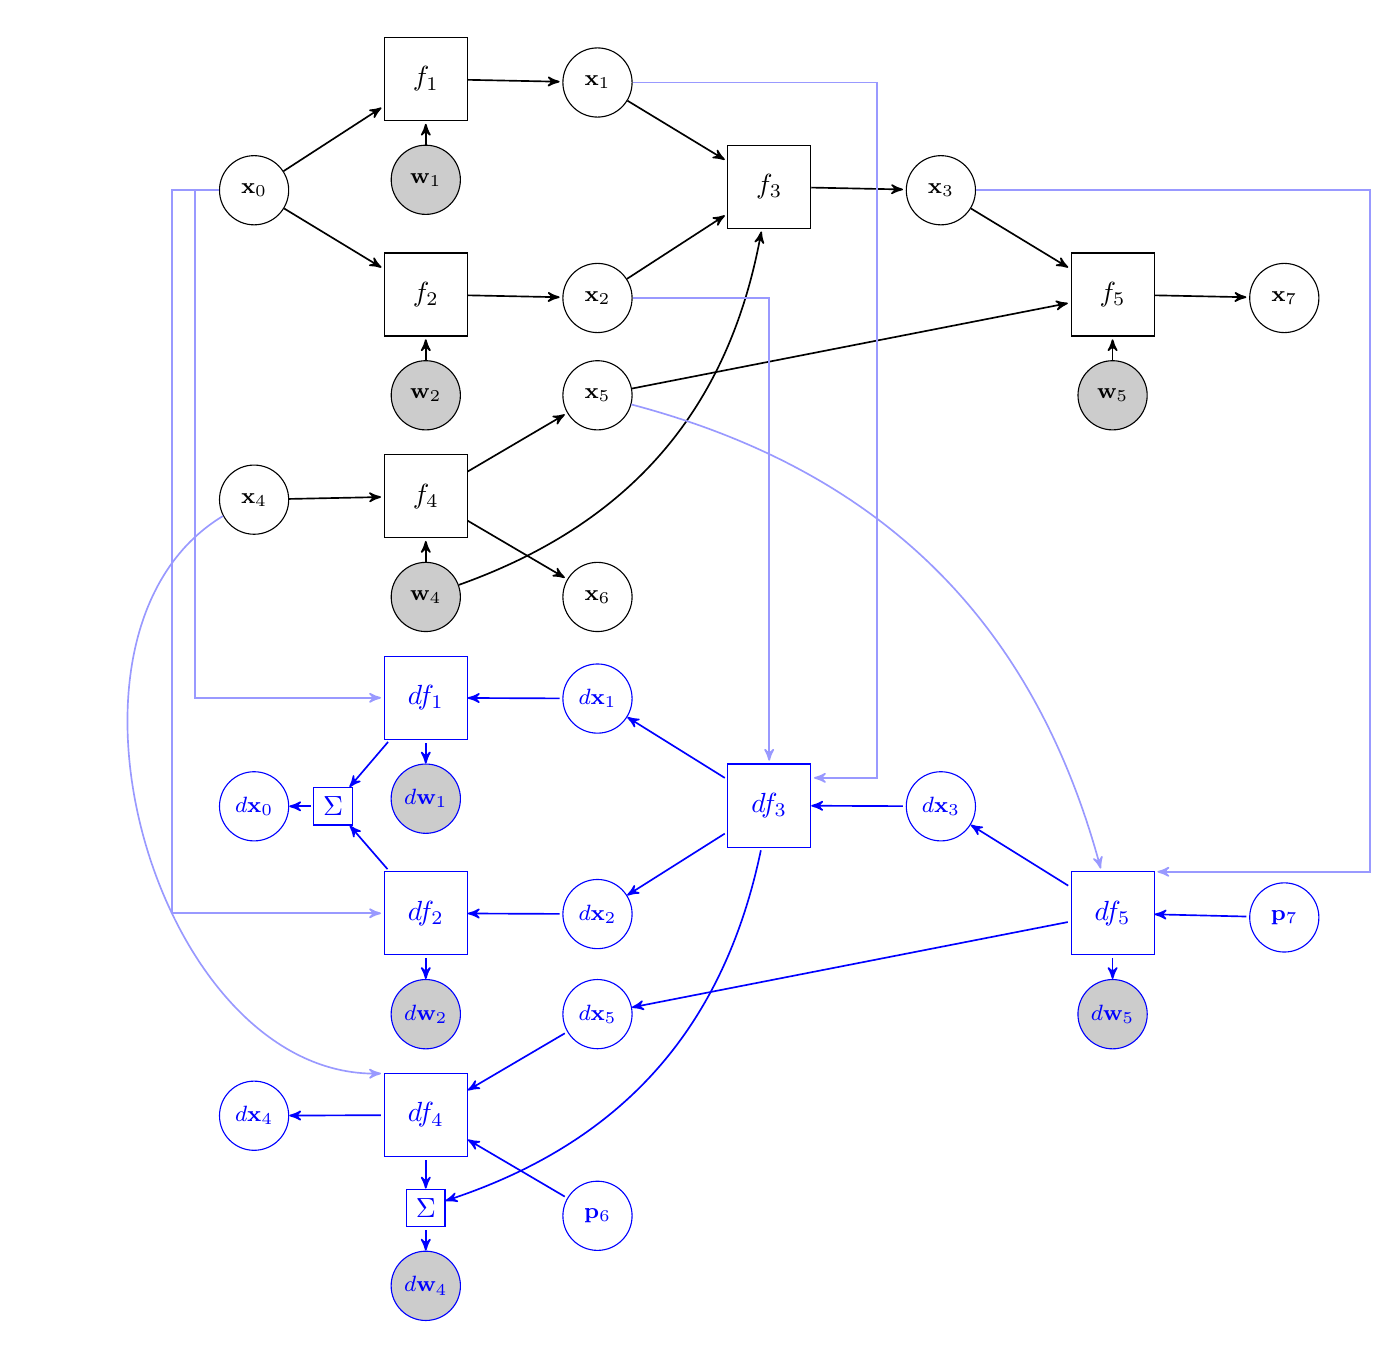
\begin{tikzpicture}[auto, node distance=0.3cm]
		\matrix (m) [matrix of math nodes, 
		column sep=1.2cm,
		row sep=0.3cm]
		{
			& \node (f1) [block]{f_1}; 
			& \node (x1) [datac]{\bx_1};
			\\
			\node (x0) [datac]{\bx_0};
			&
			&
			& \node (f3) [block]{f_3};
			& \node (x3) [datac]{\bx_3};
			\\
			& \node (f2) [block]{f_2}; 
			& \node (x2) [datac]{\bx_2};
			& &
			& \node (f5) [block]{f_5}; 
			& \node (x7) [datac]{\bx_7}; 
			\\
			& 
			& \node(x5) [datac]{\bx_5};
			\\
			\node (x4) [datac]{\bx_4};
			& \node (f4) [block]{f_4};
			\\
			& 
			& \node(x6) [datac]{\bx_6};
			\\
			% BP
			& \node (df1) [block,bp]{df_1}; 
			& \node (dx1) [datac,bp]{d\bx_1};
			\\
			\node (dx0) [datac,bp]{d\bx_0};
			&
			&
			& \node (df3) [block,bp]{df_3};
			& \node (dx3) [datac,bp]{d\bx_3};
			\\
			& \node (df2) [block,bp]{df_2}; 
			& \node (dx2) [datac,bp]{d\bx_2};
			& &
			& \node (df5) [block,bp]{df_5}; 
			& \node (dx7) [datac,bp]{\bp_7}; 
			\\
			& 
			& \node (dx5) [datac,bp]{d\bx_5};
			\\
			\node (dx4) [datac,bp]{d\bx_4};
			& \node (df4) [block,bp]{df_4};
			\\
			& 
			& \node(dx6) [datac,bp]{\bp_6};
			\\
		};
		\draw[to] (x0) -- (f1);
		\draw[to] (f1) -- (x1);
		\draw[to] (x1) -- (f3);
		\draw[to] (x0) -- (f2);
		\draw[to] (f2) -- (x2);
		\draw[to] (x2) -- (f3);
		\draw[to] (f3) -- (x3);
		\draw[to] (x3) -- (f5);
		\draw[to] (f5) -- (x7);
		\draw[to] (x4) -- (f4);
		\draw[to] (f4) -- (x5);
		\draw[to] (f4) -- (x6);
		\draw[to] (x5) -- (f5);
		\node(w1) [par,below=of f1]{$\bw_1$}; \draw[to] (w1) -- (f1);
		\node(w2) [par,below=of f2]{$\bw_2$}; \draw[to] (w2) -- (f2);
		\node(w4) [par,below=of f4]{$\bw_4$}; \draw[to] (w4) -- (f4);
		\draw[to] (w4) to [bend right] (f3);
		\node(w5) [par,below=of f5]{$\bw_5$}; \draw[to] (w5) -- (f5);
		\node (dx0s) [right of=dx0,xshift=20pt,draw,rectangle,bp]{$\Sigma$};
		\draw[from,bp] (dx0) -- (dx0s);
		\draw[from,bp] (dx0s) -- (df1);
		\draw[from,bp] (df1) -- (dx1);
		\draw[from,bp] (dx1) -- (df3);
		\draw[from,bp] (dx0s) -- (df2);
		\draw[from,bp] (df2) -- (dx2);
		\draw[from,bp] (dx2) -- (df3);
		\draw[from,bp] (df3) -- (dx3);
		\draw[from,bp] (dx3) -- (df5);
		\draw[from,bp] (df5) -- (dx7);
		\draw[from,bp] (dx4) -- (df4);
		\draw[from,bp] (df4) -- (dx5);
		\draw[from,bp] (df4) -- (dx6);
		\draw[from,bp] (dx5) -- (df5);
		\node(dw1) [par,below=of df1,bp]{$d\bw_1$}; \draw[from,bp] (dw1) -- (df1);
		\node(dw2) [par,below=of df2,bp]{$d\bw_2$}; \draw[from,bp] (dw2) -- (df2);
		\node(dw4s) [below of=df4,draw,rectangle,bp,yshift=-25pt]{$\Sigma$}; \draw[from,bp] (dw4s) -- (df4);
		\node(dw4) [par,below=of dw4s,bp]{$d\bw_4$}; \draw[from,bp] (dw4) -- (dw4s);
		\draw[from,bp] (dw4s) to [bend right,bp] (df3);
		\node(dw5) [par,below=of df5,bp]{$d\bw_5$}; \draw[from,bp] (dw5) -- (df5);
		%
		\draw[to,bpl] (x0) -| ([xshift=-0.3cm]x0.west) |- (df1);
		\draw[to,bpl] (x0) -| ([xshift=-0.6cm]x0.west) |- (df2);
		\draw[to,bpl] (x1) -| ([xshift=4cm]x1.west) |- ([yshift=10pt]df3.east);
		\draw[to,bpl] (x2) -| (df3);
		\draw[to,bpl] (x3) -| ([xshift=+5cm]x3.east) |- ([yshift=15pt]df5.east);
		\draw[to,bpl] (x4) to [bend right=75] ([yshift=15pt]df4.west);
		\draw[to,bpl] (x5) to [bend left] (df5);
		\end{tikzpicture}
	\end{center}
	\vspace{-1em}
	\caption{\textbf{Backpropagation network for a DAG.}}\label{f:dagbp}
\end{figure}

% ------------------------------------------------------------------
\paragraph{DAG backpropagation networks}\label{s:bpnets-dag}
% ------------------------------------------------------------------

Just like for sequences, backpropagation in DAGs can be implemented as a corresponding BP-reversed DAG. To construct the reversed DAG:
\begin{enumerate}
	\item For each layer $f_l$, and variable/parameter $\bx_t$ and $\bw_l$, create a corresponding layer $df_l$ and variable/parameter $d\bx_t$ and $d\bw_l$.
	\item If a variable $\bx_t$ (or parameter $\bw_l$) is an input of $f_l$, then it is an input of $df_l$ as well.
	\item If a variable $\bx_t$ (or parameter $\bw_l$) is an input of $f_l$, then the variable $d\bx_t$ (or the parameter $d\bw_l$) is an output $df_l$.
	\item In the previous step, if a variable $\bx_t$ (or parameter $\bw_l$) is input to two or more layers in $f$, then $d\bx_t$ would be the output of two or more layers in the reversed network, which creates a conflict. Resolve these conflicts by inserting a summation layer that adds these contributions (this corresponds to the summation in the BP update equation \eqref{e:bp-update}).
\end{enumerate}
The BP network corresponding to the DAG of \fref{f:dag} is given in \fref{f:dagbp}.


\subsection{ImageNet}\label{s:imagenet}
One of the greatest problems in AI has been in working with images and visual input. As we learned in \sref{s:cnn-structure}, convolutional neural networks are very effective at doing this. One of the great challenges that has pushed this field forward is ImageNet. ImageNet is a classification challenge where 1 million images are given and must be classified. Many groups all over the world strive to improve modern AI technology in order to top the charts annually. In order to produce more succesful results, many optimizations have been done to the standard neural network.

\subsubsection{Softmax}

The first challenge in this is how we can optimize determining which class something is. At the end of the network, we have one neuron per each output class (say 2 with dog and cat). We want to know which output class the image is. In simple cases, you can just take the highest. However, ImageNet allows you to take your top 5 best guesses since many classes turn out to be similar with thousands of classes (say different breeds of dogs). We want a way to estimate the probability of each label. To do this, we use the softmax layer, described in \sref{s:softmax}.

\subsubsection{VGG16}
\begin{figure}[H]
	\centering
	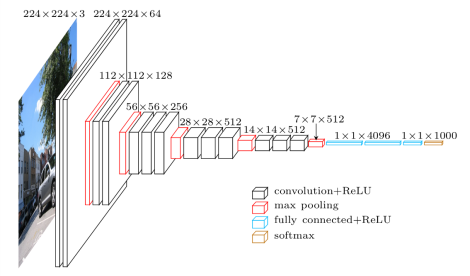
\includegraphics[scale=0.5]{images/vgg16}
	\caption{VGG16 Convolutional Network}
	\label{f:vgg16}
\end{figure}

One of the first networks that performed well combining all this so far was vgg16 \cite{pateria1990enhanced}. This network was able to classify images across thousands of categories with 90 percent accuracy given top 5 class guesses and 70.5 percent with top 1. This structure is still commonly used for many modern problems and has the benefits of being simple and easy to train. It has a slightly more powerful older cousin called vgg19 which is also very popular.

\subsubsection{ResNet}\label{s:imagenet-resnet}
\begin{figure}[H]
	\centering
	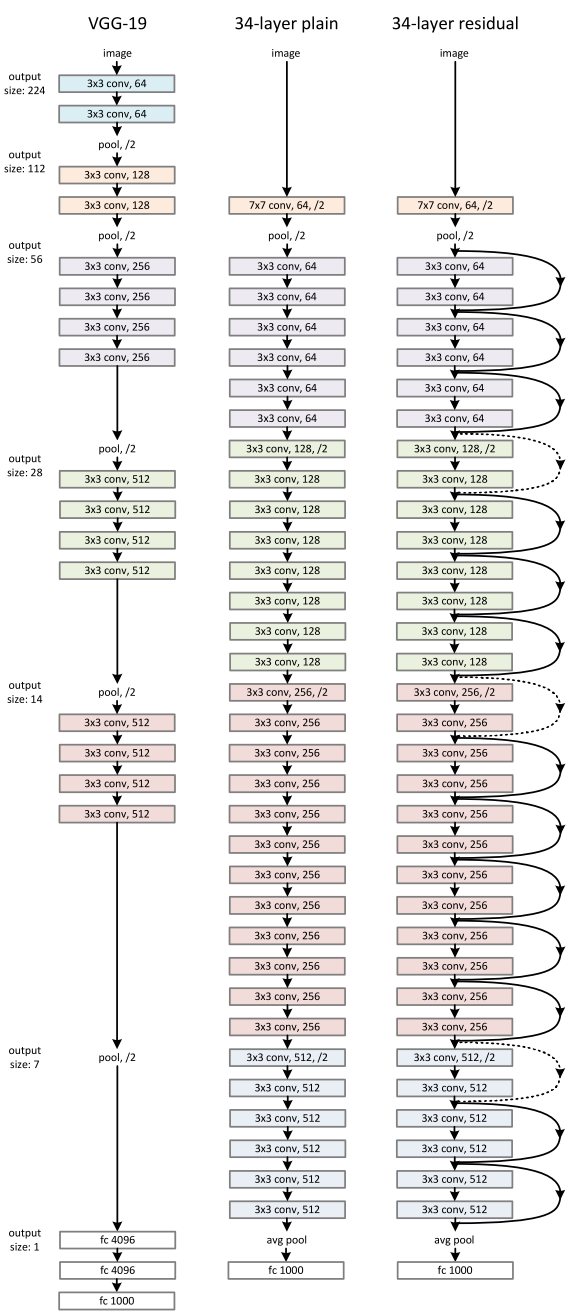
\includegraphics[width=0.65\textwidth]{images/resnetvsvgg}
	\caption{Resnet vs VGG19}
	\label{f:imagenet-resnet}
\end{figure}

For some years, the trend in machine learning was always adding more layers. With the constant improvement in GPUs, if something didn't work now, the solution was to wait a year and add more layers. However, one big issue that exists with this is the vanishing gradient. At some point, the connection between the input and the output is too spaced away and the network can no longer learn significant features at the lower layers. However, we know that deeper networks can learn more complex features more easily and are much better suited to handle hard problems. To solve this, researchers produced residual connections \cite{he2016deep}, which are described in \sref{s:blocks-resnet}.

As you can see, ResNet allows for much greater depth compared to VGG. This, too, is the smallest size of ResNet. Typical applications use ResNet-50 at least and high-end ones use ResNet-152. The sheer power of these structures has allowed for 92.9 percent accuracy on ImageNet and the usage of training on fancy GPUs with lots of data.

We indeed used ResNet-50 as backbone for our \maskrcnn.


\subsubsection{Inception}\label{s:imagenet-inception}
\begin{figure}[H]
	\centering
	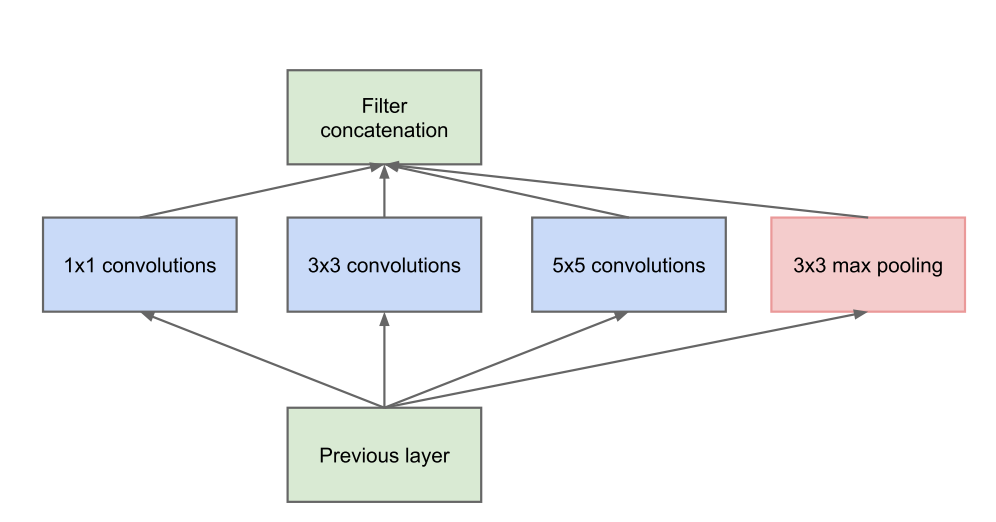
\includegraphics[scale=0.5]{images/inception}
	\caption{Parallel Layers in Residual Note in Inception Neural Network.}
	\label{f:imagenet-inception}
\end{figure}

The last major improvement in recent years in image classification has been in the usage of multiple parallel layers in each residual node. Each of these sets of layers, as seen in the image above, contains different filter sizes, allowing for a varying size of features to be extracted. From this, each residual node can learn much more and increased information can be packed in. This has culminated in Inception-ResNet structures capable of producing results more accurate than humans on image classification.

Coincidentally, Tesla's neural network used for its Autonomous Driving features called “Autopilot", currently, as of V9 software (2019), still uses Inception V1.
\begin{quote}[teslamotorsclub.com]{jimmy-d}
	The V9 network takes 1280x960 images with 3 color channels and 2 frames per camera from, for example, the main camera. That’s 1280x960x3x2 as an input, or 7.3M. The V8 main camera was 640x416x2 or 0.5M - 13x less data.
\end{quote}

\subsubsection{To the Future}
In large part, following these advances, image classification has been solved. Without massive amounts of data, performance enhancements will largely be negligible. However, as these structures have gotten bigger, they have also gotten slower and slower. In recent years, the next step has been in breaking down multiple objects and analyzing complex images, as in \sref{s:nnevo}.




% ------------------------------------------------------------------
\subsection{Computational blocks}\label{s:blocks}
% ------------------------------------------------------------------

This section describes the individual computational blocks supported by \maskrcnn. The interface of a CNN computational block $<block>$ is designed after the discussion in \sref{s:fundamentals}. We can see a block as a function $y =<block>(x,w)$ that takes as input  arrays $x$ and $w$ representing the input data and parameters and returns an array $y$ as output. In general, $x$ and $y$ are 4D real arrays packing $N$ maps or images, as discussed above, whereas $w$ may have an arbitrary shape.

The function implementing each block is capable of working in the backward direction as well, in order to compute derivatives. This is done by passing a third optional argument $dzdy$ representing the derivative of the output of the network with respect to $\by$; in this case, the function returns the derivatives $[dzdx,dzdw] = <block>(x,w,dzdy)$ with respect to the input data and parameters. The arrays $dzdx$, $dzdy$ and $dzdw$ have the same dimensions of $x$, $y$ and $w$ respectively (see \sref{s:back}).

Different functions may use a slightly different syntax, as needed: many functions can take additional optional arguments, specified as property-value pairs; some do not have parameters  $w$ (e.g. a rectified linear unit); others can take multiple inputs and parameters, in which case there may be more than one $x$, $w$, $dzdx$, $dzdy$ or $dzdw$.

% ------------------------------------------------------------------
\subsubsection{Convolution}\label{s:convolution}
% ------------------------------------------------------------------

\begin{figure}[H]
	\centering
	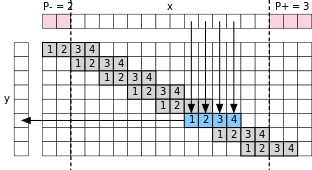
\includegraphics[width=0.7\textwidth]{figures/svg/conv}
	\caption{\textbf{Convolution.} The figure illustrates the process of filtering a 1D signal $\bx$ by a filter $f$ to obtain a signal $\by$. The filter has $H'=4$ elements and is applied with a stride of $S_h =2$ samples. The purple areas represented padding $P_-=2$ and $P_+=3$ which is zero-filled. Filters are applied in a sliding-window manner across the input signal. The samples of $\bx$ involved in the calculation of a sample of $\by$ are shown with arrow. Note that the rightmost sample of $\bx$  is never processed by any filter application due to the sampling step. While in this case the sample is in the padded region, this can happen also without padding.}\label{f:conv}
\end{figure}

The convolutional block is implemented by the function $vl_nnconv$. $y=vl_nnconv(x,f,b)$ computes the convolution of the input map $\bx$ with a bank of $D''$ multi-dimensional filters $\bff$ and biases $b$. Here
\[
\bx\in\real^{H \times W \times D}, \quad
\bff\in\real^{H' \times W' \times D \times D''}, \quad
\by\in\real^{H'' \times W'' \times D''}.
\]
The process of convolving a signal is illustrated in \sref{f:conv} for a 1D slice. Formally, the output is given by
\[
y_{i''j''d''}
=
b_{d''}
+
\sum_{i'=1}^{H'}
\sum_{j'=1}^{W'}
\sum_{d'=1}^D
f_{i'j'd} \times x_{i''+i'-1,j''+j'-1,d',d''}.
\]
The call $vl_nnconv(x,f,[])$ does not use the biases. Note that the function works with arbitrarily sized inputs and filters (as opposed to, for example, square images). 

\subparagraph{Padding and stride.} $conv$ allows to specify  top-bottom-left-right paddings $(P_h^-,P_h^+,P_w^-,P_w^+)$ of the input array and subsampling strides $(S_h,S_w)$ of the output array:
\[
y_{i''j''d''}
=
b_{d''}
+
\sum_{i'=1}^{H'}
\sum_{j'=1}^{W'}
\sum_{d'=1}^D
f_{i'j'd} \times x_{S_h (i''-1)+i'-P_h^-, S_w(j''-1)+j' - P_w^-,d',d''}.
\]
In this expression, the array $\bx$ is implicitly extended with zeros as needed.

\subparagraph{Output size.} $conv$ computes only the ``valid'' part of the convolution; i.e. it requires each application of a filter to be fully contained in the input support.  The size of the output is given by:
\[
H'' = 1 + \left\lfloor \frac{H - H' + P_h^- + P_h^+}{S_h} \right\rfloor.
\]
Note that the padded input must be at least as large as the filters: $H +P_h^- + P_h^+ \geq H'$.

\subparagraph{Receptive field size and geometric transformations.} Very often it is useful to geometrically relate the indexes of the various array to the input data (usually images) in terms of coordinate transformations and size of the receptive field (i.e. of the image region that affects an output).

\subparagraph{Filter groups.} Filter grouping allows to group channels of the input array $\bx$ and apply different subsets of filters to each group. This takes as input a bank of $D''$ filters $\bff\in\real^{H'\times W'\times D'\times D''}$ such that $D'$ divides the number of input dimensions $D$. These are treated as $g=D/D'$ filter groups; the first group is applied to dimensions $d=1,\dots,D'$ of the input $\bx$; the second group to dimensions $d=D'+1,\dots,2D'$ and so on. Note that the output is still an array $\by\in\real^{H''\times W''\times D''}$.

An application of grouping is implementing the Krizhevsky and Hinton network (ImageNet)~\cite{krizhevsky12imagenet} which uses two such streams. Another application is sum pooling; in the latter case, one can specify $D$ groups of $D'=1$ dimensional filters identical filters of value 1 (however, this is considerably slower than calling the dedicated pooling function as given in \sref{s:pooling}).

\subparagraph{Dilation.} $conv$ allows kernels to be spatially dilated on the fly by inserting zeros between elements. For instance, a dilation factor $d=2$ causes the 1D kernel $[f_1,f_2]$ to be implicitly transformed into the kernel $[f_1,0,f_2]$. Under this notation, $d-1$ zeros are inserted between filter elements (and consequently, a dilation factor of $1$ has no effect). Thus, with dilation factors $d_h,d_w$, a filter of size $(H_f,W_f)$ is equivalent to a filter of size:
\[
H' = d_h(H_f - 1) + 1,
\qquad
W' = d_w(W_f - 1) + 1.
\]
With dilation, the convolution becomes:
\[
y_{i''j''d''}
=
b_{d''}
+
\sum_{i'=1}^{H_f}
\sum_{j'=1}^{W_f}
\sum_{d'=1}^D
f_{i'j'd} \times x_{
	S_h (i''-1)+d_h(i'-1)-P_h^-+1,
	S_w (j''-1)+d_w(j'-1)-P_w^-+1,
	d',d''}.
\]


% ------------------------------------------------------------------
\subsubsection{Convolution transpose (deconvolution)}\label{s:convt}
% ------------------------------------------------------------------

% TODO delete deconvolution?

\begin{figure}[t]
	\centering
	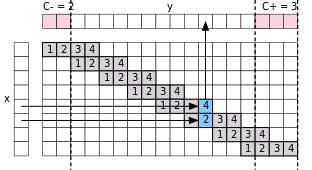
\includegraphics[width=0.7\textwidth]{figures/svg/convt}
	\caption{\textbf{Convolution transpose.} The figure illustrates the process of filtering a 1D signal $x$ by a filter $f$ to obtain a signal $y$. The filter is applied as a sliding-window, forming a pattern which is the transpose of the one of \sref{f:conv}. The filter has $H'=4$ samples in total, although each filter application uses two of them (blue squares) in a circulant manner. The purple areas represent crops with $C_-=2$ and $C_+=3$ which are discarded. The arrows exemplify which samples of $x$ are involved in the calculation of a particular sample of $y$. Note that, differently from the forward convolution \sref{f:conv}, there is no need to add padding to the input array; instead, the convolution transpose filters can be seen as being applied with maximum input padding (more would result in zero output values), and the latter can be reduced by cropping the output instead.}\label{f:convt}
\end{figure}

The \emph{convolution transpose} block (sometimes referred to as ``deconvolution'') is the transpose of the convolution block described in \sref{s:convolution}. We'll refere to it by the name $convt$.

In order to understand convolution transpose, let:
\[
\bx\in\real^{H \times W \times D}, \quad
\bff\in\real^{H' \times W' \times D \times D''}, \quad
\by\in\real^{H'' \times W'' \times D''}, \quad
\]
be the input tensor, filters, and output tensors. Imagine operating in the reverse direction by using the filter bank $\bff$ to convolve the output $\by$ to obtain the input $\bx$, using the definitions given in~\sref{s:convolution} for the convolution operator; since convolution is linear, it can be expressed as a matrix $M$ such that  $\vv \bx = M \vv\by$; convolution transpose computes instead $\vv \by = M^\top \vv \bx$. This process is illustrated for a 1D slice in \sref{f:convt}.

There are two important applications of convolution transpose. The first one is the so called \emph{deconvolutional networks}~\cite{zeiler14visualizing} and other networks such as convolutional decoders that use the transpose of a convolution. The second one is implementing data interpolation. In fact, as the convolution block supports input padding and output downsampling, the convolution transpose block supports input upsampling and output cropping.

Convolution transpose can be expressed in closed form in the following rather unwieldy expression:
\begin{multline}\label{e:convt}
y_{i''j''d''} =
\sum_{d'=1}^{D}
\sum_{i'=0}^{q(H',S_h)}
\sum_{j'=0}^{q(W',S_w)}
f_{
	1+ S_hi' + m(i''+ P_h^-, S_h),\ %
	1+ S_wj' + m(j''+ P_w^-, S_w),\ %
	d'',
	d'
}
\times \\
x_{
	1 - i' + q(i''+P_h^-,S_h),\ %
	1 - j' + q(j''+P_w^-,S_w),\ %
	d'
}
\end{multline}
where
\[
m(k,S) = (k - 1) \bmod S,
\qquad
q(k,n) = \left\lfloor \frac{k-1}{S} \right\rfloor,
\]
$(S_h,S_w)$ are the vertical and horizontal \emph{input upsampling factors},  $(P_h^-,P_h^+,P_h^-,P_h^+)$ the \emph{output crops}, and $\bx$ and $\bff$ are zero-padded as needed in the calculation. Note also that filter $k$ is stored as a slice $\bff_{:,:,k,:}$ of the 4D tensor $\bff$.

The height of the output array $\by$ is given by
\[
H'' = S_h (H - 1) + H' -P^-_h - P^+_h.
\]
A similar formula holds true for the width. These formulas are derived in \sref{s:receptive-convolution-transpose} along with an expression for the receptive field of the operator.

We now illustrate the action of convolution transpose in an example (see also \sref{f:convt}).  Consider a 1D slice in the vertical direction, assume that the crop parameters are zero, and that $S_h>1$. Consider the output sample $y_{i''}$ where the index $i''$ is chosen such that $S_h$ divides $i''-1$; according to~\eqref{e:convt}, this sample is obtained as a weighted summation of $x_{i'' / S_h},x_{i''/S_h-1},...$ (note that the order is reversed). The weights are the filter elements $f_1$, $f_{S_h}$,$f_{2S_h},\dots$ subsampled with a step of $S_h$. Now consider computing the element $y_{i''+1}$; due to the rounding in the quotient operation $q(i'',S_h)$, this output sample is obtained as a weighted combination of the same elements of the input $x$ that were used to compute $y_{i''}$; however, the filter weights are now shifted by one place to the right: $f_2$, $f_{S_h+1}$,$f_{2S_h+1}$, $\dots$. The same is true for $i''+2, i'' + 3,\dots$ until we hit $i'' + S_h$. Here the cycle restarts after shifting $\bx$ to the right by one place. Effectively, convolution transpose works as an \emph{interpolating filter}.

\paragraph{Residual Connections}\label{s:blocks-resnet}
\begin{figure}[H]
	\centering
	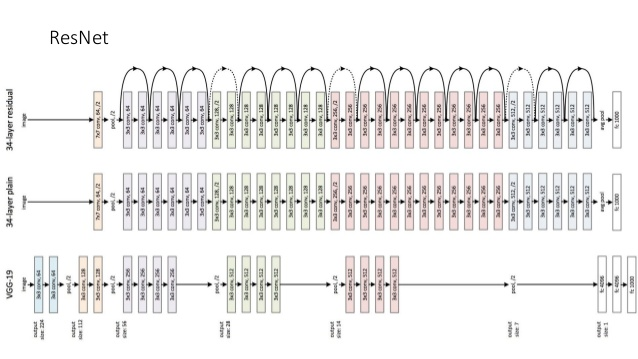
\includegraphics[scale=0.5]{images/resnet}
	\caption{Single Residual Block}
	\label{f:blocks-res}
\end{figure}
Residual connections are essentially the nodes in \fref{f:blocks-res}, which consist of a set of layers. Each node extracts some features from the raw image and then combines this information with the original input to pass into the subsequent layer. In this way, features can be extracted in depth and subsequent layers can maintain access to the original information.

Residual connections are used in ResNet, described in \sref{s:imagenet-resnet}.


% ------------------------------------------------------------------
\subsubsection{Spatial pooling}\label{s:pooling}
% ------------------------------------------------------------------

Pooling can be max or avg pooling. The \emph{max pooling} operator computes the maximum response of each feature channel in a $H' \times W'$ patch
\[
y_{i''j''d} = \max_{1\leq i' \leq H', 1 \leq j' \leq W'} x_{i''+i'-1,j''+j'-1,d}.
\]
resulting in an output of size $\by\in\real^{H''\times W'' \times D}$, similar to the convolution operator of \sref{s:convolution}. Average-pooling computes the average of the values instead:
\[
y_{i''j''d} = \frac{1}{W'H'}
\sum_{1\leq i' \leq H', 1 \leq j' \leq W'} x_{i''+i'-1,j''+j'-1,d}.
\]


\subparagraph{Padding and stride.} Similar to the convolution operator of \sref{s:convolution}, $pool$ supports padding the input; however, the effect is different from padding in the convolutional block as pooling regions straddling the image boundaries are cropped. For max pooling, this is equivalent to extending the input data with $-\infty$; for sum pooling, this is similar to padding with zeros, but the normalization factor at the boundaries is smaller to account for the smaller integration area.
\pagebreak
% ------------------------------------------------------------------
\subsubsection{RoI Pooling}\label{s:roi-pooling}
% ------------------------------------------------------------------

RoI Pooling is similar to max-pooling, \sref{s:pooling}. Let's say our convolutional feature map has size $8\times8$, and our first fully connected layer needs an input of size $2\times2$. Region of Interest Pooling would then follow the figures below.

\begin{figure}[htbp]
	\centering
	\begin{minipage}{0.5\textwidth}
		\centering
		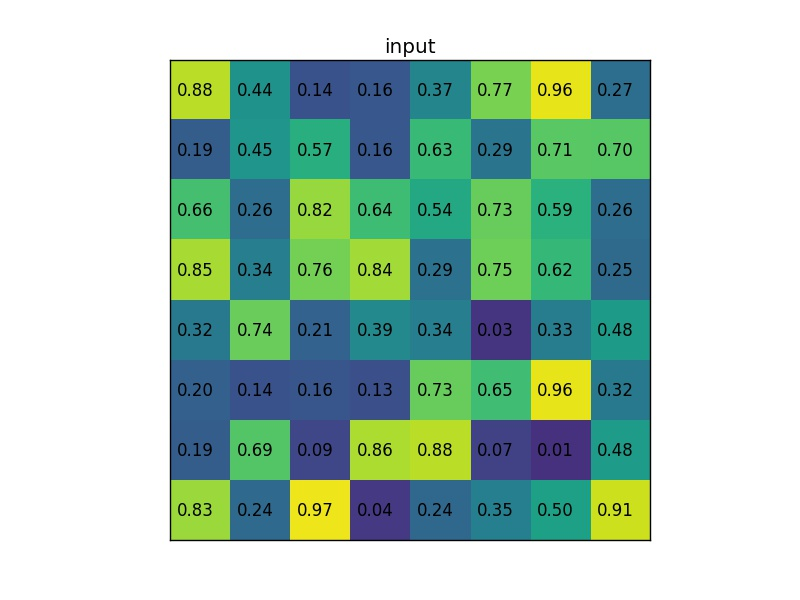
\includegraphics[width=1.1\textwidth]{images/roipool1.jpg} % first
		%figure itself
	\end{minipage}\hfill
	\begin{minipage}{0.5\textwidth}
		\centering
		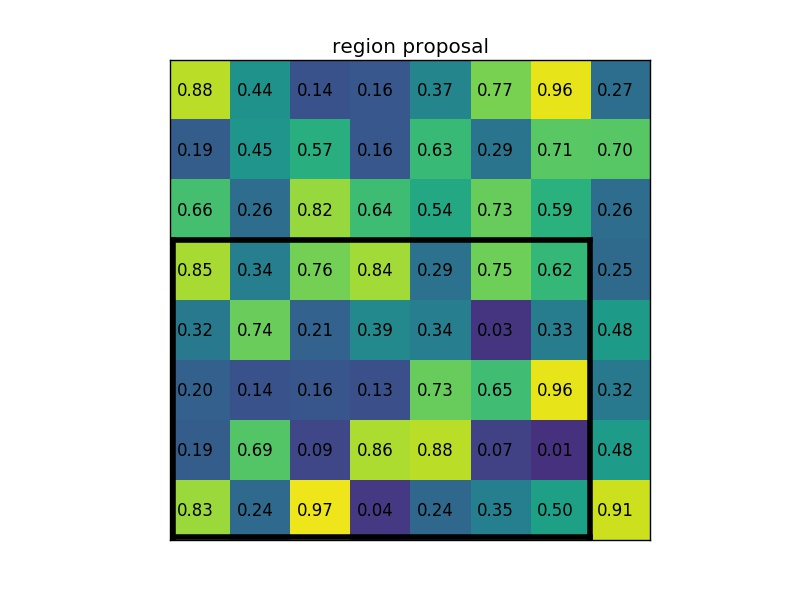
\includegraphics[width=1.1\textwidth]{images/roipool2.jpg} %second
		%figure itself
	\end{minipage}
\end{figure}

\begin{figure}[htbp]
	\centering
	\begin{minipage}{0.5\textwidth}
		\centering
		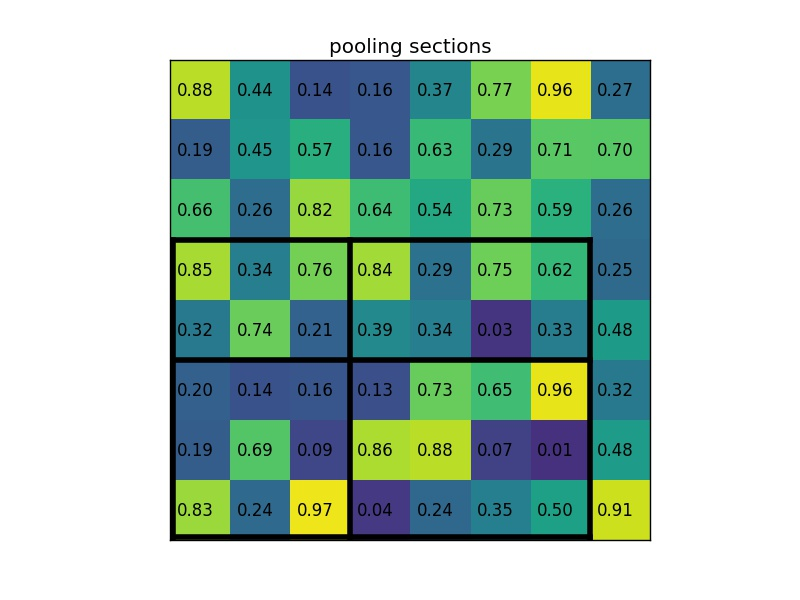
\includegraphics[width=1.1\textwidth]{images/roipool3.jpg} % first
		%figure itself
	\end{minipage}\hfill
	\begin{minipage}{0.5\textwidth}
		\centering
		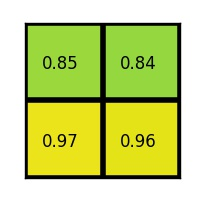
\includegraphics[width=0.5\textwidth]{images/roipool4.jpg} %second
		%figure itself
		\caption{$2\times2$ output.}
	\end{minipage}
\end{figure}

Simply put, if an $N\times N$ output is desired, the proposed region (black rectangle in the upper-right image) is divided into an $N\times N$ grid. When the region dimensions are not divisible by $N$, the sections of the grid will not all contain the same number of pixels. From each section, we take the greatest pixel value, and arrange these values in an $N\times N$ grid, forming our output. This output is then passed through the fully connected layers.


RoI Pooling is used in Fast \cite{Girshick_2015} and Faster R-CNN, \sref{s:nnevo-fastrcnn}
\pagebreak
\subsubsection{RoIAlign}\label{s:roi-align}
RoAlign is simply a more precise version of RoI Pooling, described above in \sref{s:roi-pooling}

\begin{figure}[H]
	\centering
	\begin{minipage}{0.5\textwidth}
		\centering
		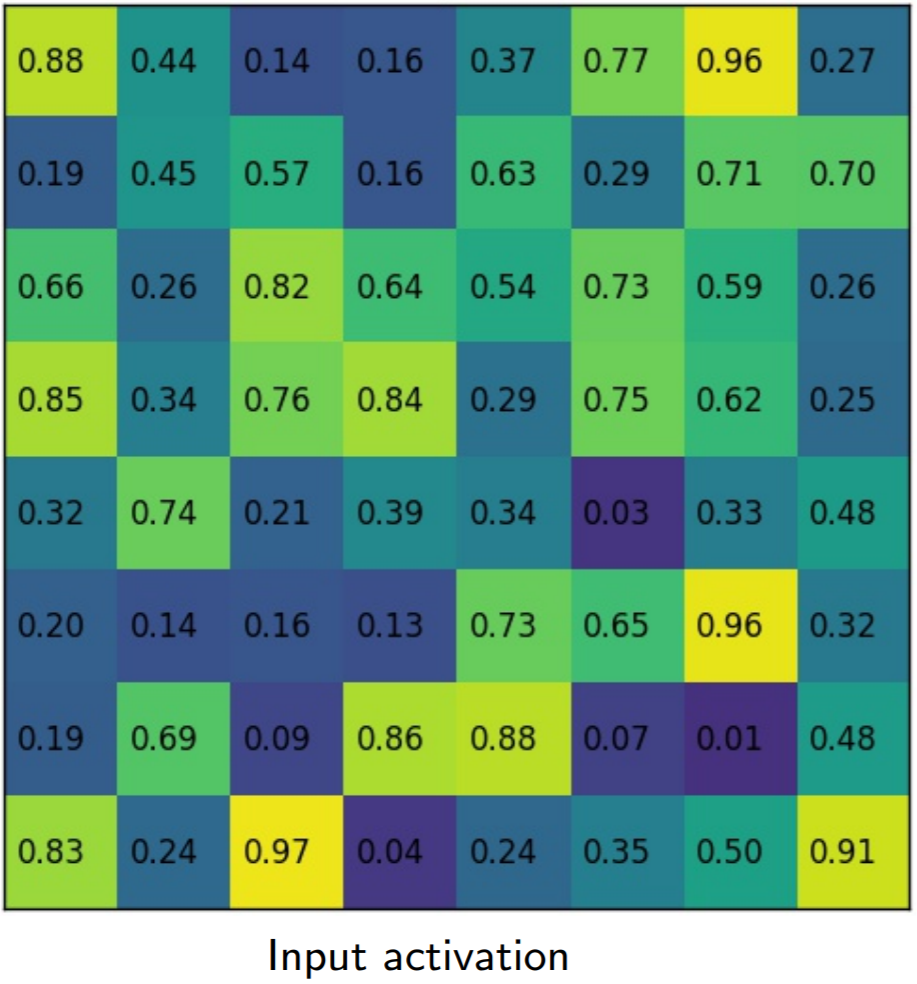
\includegraphics[width=0.8\textwidth]{images/roialign1.PNG} % first
		%figure itself
	\end{minipage}\hfill
	\begin{minipage}{0.5\textwidth}
		\centering
		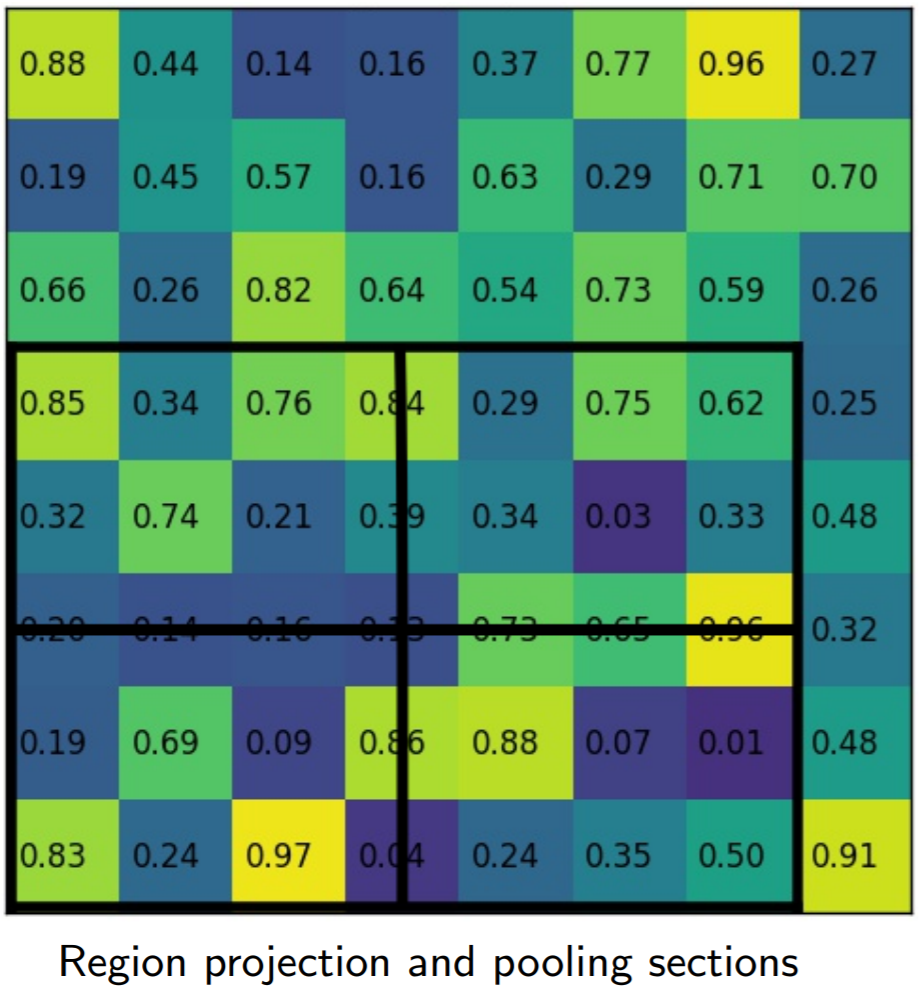
\includegraphics[width=0.8\textwidth]{images/roialign2.PNG} %second
		%figure itself
	\end{minipage}
\end{figure}

\begin{figure}[H]
	\centering
	\begin{minipage}{0.5\textwidth}
		\centering
		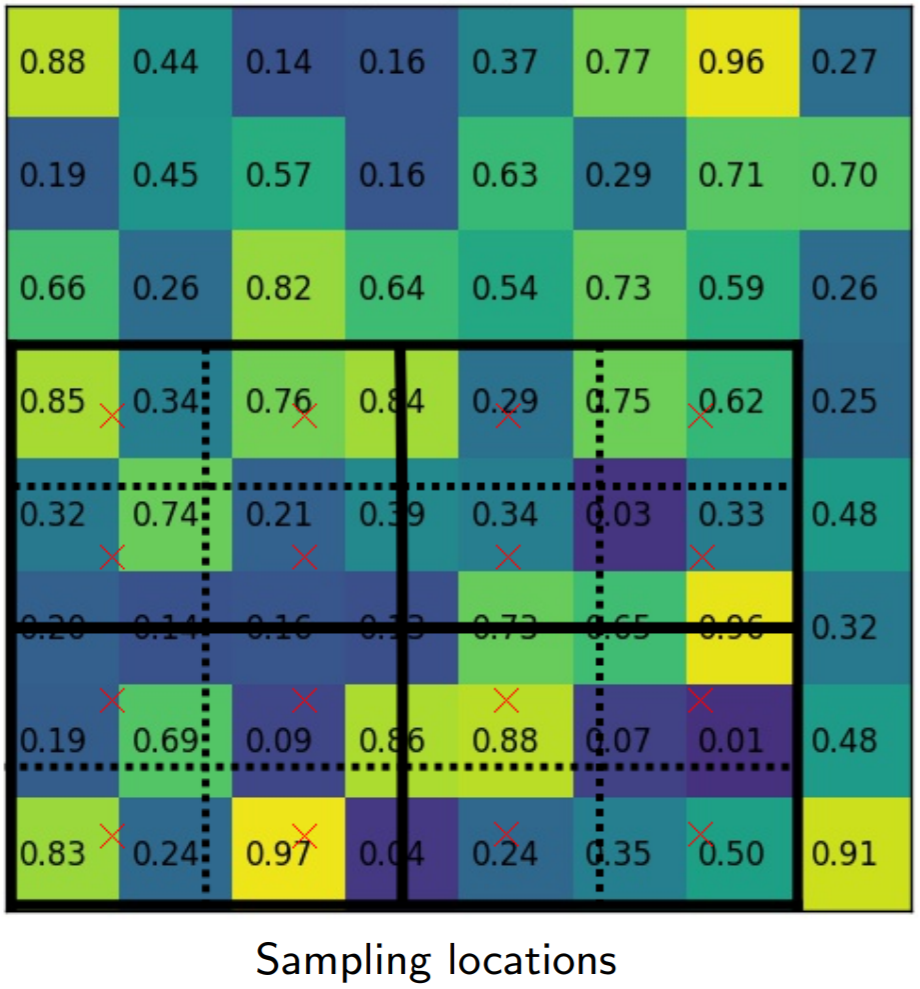
\includegraphics[width=0.8\textwidth]{images/roialign3.PNG} % first
		%figure itself
	\end{minipage}\hfill
	\begin{minipage}{0.5\textwidth}
		\centering
		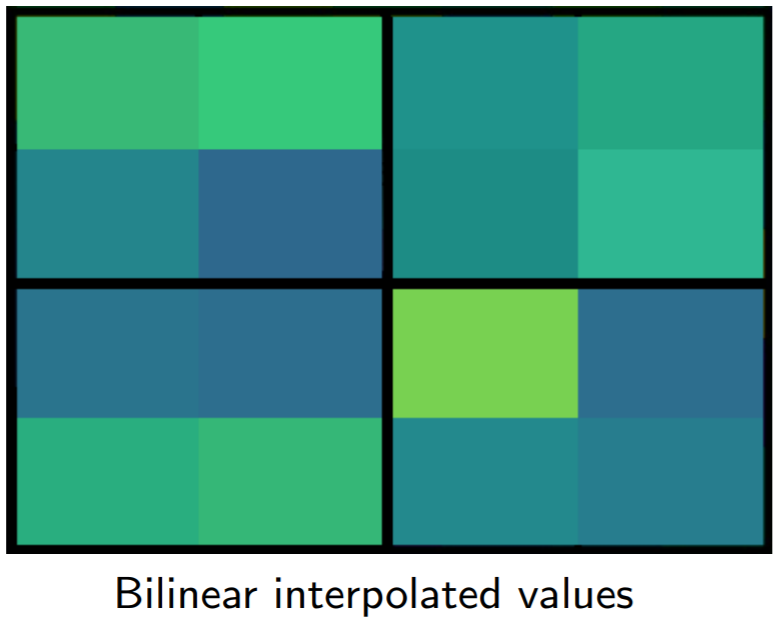
\includegraphics[width=0.8\textwidth]{images/roialign4.PNG} %second
		%figure itself
		\caption{$2\times2$ values per cell.}
	\end{minipage}
\end{figure}

\begin{figure}[H]
	\centering
	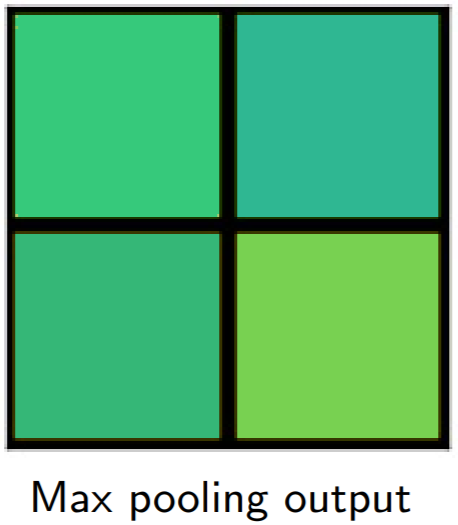
\includegraphics[scale=0.35]{images/roialign5.PNG}
\end{figure}

Simply put, if an $N\times N$ output is desired, the proposed region (black rectangle in the upper-right image) is divided into an $N\times N$ grid. Unlike RoI Pooling, these regions will contain the exact same number of pixels, so we will often have fractional pixels. From each grid cell, we sample four regions as shown by the red $\times$ marks in the third image. We then subdivide each grid cell into four subcells, each centered on an $\times$. We perform bilinear interpolation to get a single value for each subregion, or four values for each cell. These values are shown in the fourth image. Finally, we perform a simple max pooling [\sref{s:pooling}] on the bilinear interpolated values, taking the maximum value per cell to reach an $N\times N$ output. 

You can jump back to \sref{s:maskrcnn} or understand in detail what is Bilinear Interpolation below in \sref{s:roi-bi}.

\paragraph{Bilinear Interpolation}\label{s:roi-bi}
Bilinear interpolation is fairly trivial. It is best understood visually. Simply put, the bilinearly interpolated value at the black spot is the sum of the values of each of the four colors multiplied by the areas of their respective rectangles, divided by the total area.

\begin{figure}[htbp]
	\centering
	\begin{minipage}{0.4\textwidth}
		\centering
		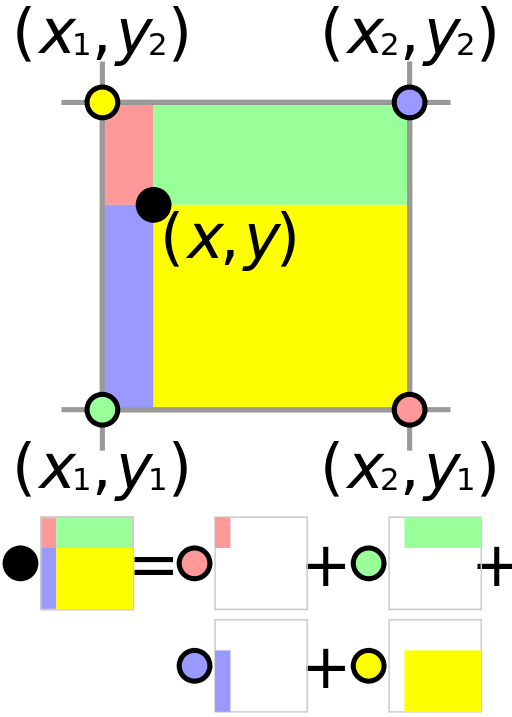
\includegraphics[width=0.8\textwidth]{images/bilinear.png} % first
		%figure itself
	\end{minipage}\hfill
	\begin{minipage}{0.6\textwidth}
		\centering
		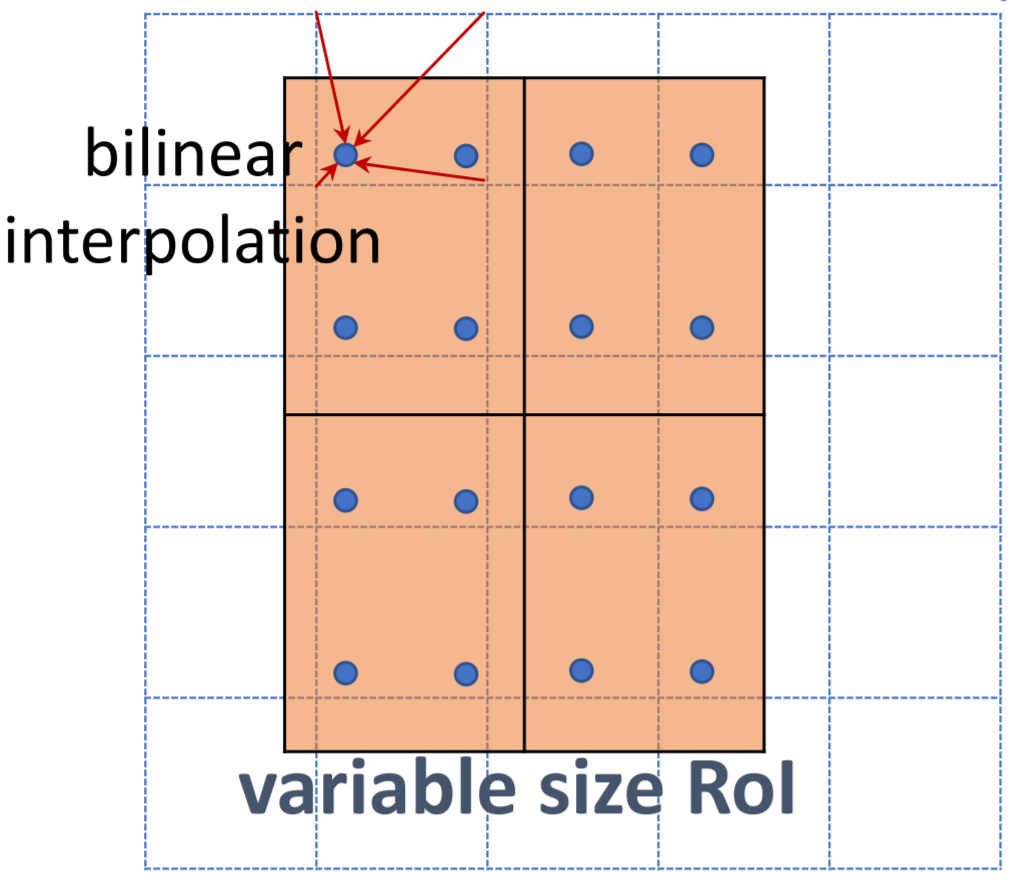
\includegraphics[width=0.8\textwidth]{images/roibilinear.PNG} %second
		%figure itself
		\caption{Bilinear interpolation for RoIAlign.}
	\end{minipage}
\end{figure}

Note how in the figure on the left, the red pixel value corresponds to the smaller area opposite the pixel. This is because closer pixels (like the yellow one) have greater weighting.
The figure on the right makes it clear how bilinear interpolation is implementaed in RoIAlign. At each blue dot (represented with a red $\times$ in the figures on the previous page), we take the closest 4 pixel values and multiply them by the respective areas.

And that's all RoIAlign is. It achieves the same goal as RoI Pooling, which is to take a region of any shape and create a fixed output. However, because we are using fractional pixels, we can get much better alignment. This simple change resulted in considerable accuracy improvements for \maskrcnn, described in \sref{s:maskrcnn}

% ------------------------------------------------------------------
\subsubsection{Activation functions}\label{s:activation}
% ------------------------------------------------------------------

% ------------------------------------------------------------------
\paragraph{Rectified Linear Unit}\label{s:relu}
% ------------------------------------------------------------------
(ReLU):
	\[
	y_{ijd} = \max\{0, x_{ijd}\}.
	\]
	

% ------------------------------------------------------------------
\paragraph{Sigmoid}\label{s:sigmoid}
% ------------------------------------------------------------------
The sigmoid operator is:
	\[
	y_{ijd} = \sigma(x_{ijd}) = \frac{1}{1+e^{-x_{ijd}}}.
	\]
% ------------------------------------------------------------------
\paragraph{Softmax}\label{s:softmax}
% ------------------------------------------------------------------

The softmax operator is:
\[
y_{ijk} = \frac{e^{x_{ijk}}}{\sum_{t=1}^D e^{x_{ijt}}}.
\]
Note that the operator is applied across feature channels and in a convolutional manner at all spatial locations. Softmax can be seen as the combination of an activation function (exponential) and a normalization operator. 

This function essentially takes the sum of all the outputs and raises it to $e$ to make it positive. It then calculates the probability of each label by taking its value raised to $e$ over the total sum just calculated, which essentially shows us how much of the sum it consists of, nicely giving us a probability.


% ------------------------------------------------------------------
\subsubsection{Normalization}\label{s:normalization}
% ------------------------------------------------------------------

% ------------------------------------------------------------------
\paragraph{Local response normalization (LRN)}\label{s:ccnormalization}
% ------------------------------------------------------------------

The Local Response Normalization (LRN) operator is applied independently at each spatial location and to groups of feature channels as follows:
\[
y_{ijk} = x_{ijk} \left( \kappa + \alpha \sum_{t\in G(k)} x_{ijt}^2 \right)^{-\beta},
\]
where, for each output channel $k$, $G(k) \subset \{1, 2, \dots, D\}$ is a corresponding subset of input channels. Note that input $\bx$ and output $\by$ have the same dimensions. Note also that the operator is applied uniformly at all spatial locations.


% ------------------------------------------------------------------
\paragraph{Batch normalization}\label{s:bnorm}
% ------------------------------------------------------------------

~\cite{ioffe2015} Batch normalization is somewhat different from other neural network blocks in that it performs computation across images/feature maps in a batch (whereas most blocks process different images/feature maps individually). $y = vl_nnbnorm(x, w, b)$ normalizes each channel of the feature map $\mathbf{x}$ averaging over spatial locations and batch instances. Let $T$ be the batch size; then
\[
\mathbf{x}, \mathbf{y} \in \mathbb{R}^{H \times W \times K \times T},
\qquad\mathbf{w} \in \mathbb{R}^{K},
\qquad\mathbf{b} \in \mathbb{R}^{K}.
\]
Note that in this case the input and output arrays are explicitly treated as 4D tensors in order to work with a batch of feature maps. The tensors  $\mathbf{w}$ and $\mathbf{b}$ define component-wise multiplicative and additive constants. The output feature map is given by
\[
y_{ijkt} = w_k \frac{x_{ijkt} - \mu_{k}}{\sqrt{\sigma_k^2 + \epsilon}} + b_k,
\quad
\mu_{k} = \frac{1}{HWT}\sum_{i=1}^H \sum_{j=1}^W \sum_{t=1}^{T} x_{ijkt},
\quad
\sigma^2_{k} = \frac{1}{HWT}\sum_{i=1}^H \sum_{j=1}^W \sum_{t=1}^{T} (x_{ijkt} - \mu_{k})^2.
\]


% ------------------------------------------------------------------
\paragraph{Spatial normalization}\label{s:spnorm}
% ------------------------------------------------------------------

The spatial normalization operator acts on different feature channels independently and rescales each input feature by the energy of the features in a local neighbourhood . First, the energy of the features in a neighbourhood $W'\times H'$ is evaluated
\[
n_{i''j''d}^2 = \frac{1}{W'H'}
\sum_{1\leq i' \leq H', 1 \leq j' \leq W'} x^2_{
	i''+i'-1-\lfloor \frac{H'-1}{2}\rfloor,
	j''+j'-1-\lfloor \frac{W'-1}{2}\rfloor,
	d}.
\]
In practice, the factor $1/W'H'$ is adjusted at the boundaries to account for the fact that neighbors must be cropped. Then this is used to normalize the input:
\[
y_{i''j''d} = \frac{1}{(1 + \alpha n_{i''j''d}^2)^\beta} x_{i''j''d}.
\]


% ------------------------------------------------------------------
\subsubsection{Categorical losses}\label{s:losses}
% ------------------------------------------------------------------

The purpose of a categorical loss function $\ell(\bx,\bc)$ is to compare a prediction $\bx$ to a ground truth class label $\bc$. The contribution of different samples are summed together (possibly after weighting) and the output of the loss is a scalar. \sref{s:loss-classification} losses useful for multi-class classification and the \sref{s:loss-attributes} losses useful for binary attribute prediction. 

% ------------------------------------------------------------------
\paragraph{Classification losses}\label{s:loss-classification}
% ------------------------------------------------------------------

% TODO forse mettere le losses nella nuova sezione train algorithm?

Classification losses decompose additively as follows:
\begin{equation}\label{e:addloss}
\ell(\bx,\bc) = \sum_{ijn} w_{ij1n} \ell(\bx_{ij:n}, \bc_{ij:n}).
\end{equation}
Here $\bx \in \mathbb{R}^{H \times W \times C \times N}$ and $\bc \in \{1, \dots, C\}^{H \times W \times 1 \times N}$, such that the slice $\bx_{ij:n}$ represent a vector of $C$ class scores and and $c_{ij1n}$ is the ground truth class label. The $`instanceWeights`$ option can be used to specify the tensor $\bw$ of weights, which are otherwise set to all ones; $\bw$ has the same dimension as $\bc$.

\subparagraph{Classification error.} The classification error is zero if class $c$ is assigned the largest score and zero otherwise:
\begin{equation}\label{e:loss-classerror}
\ell(\bx,c) = \mathbf{1}\left[c \not= \argmax_k x_c\right].
\end{equation}
Ties are broken randomly.

\subparagraph{Top-$K$ classification error.} The top-$K$ classification error is zero if class $c$ is within the top $K$ ranked scores:
\begin{equation}\label{e:loss-classerror}
\ell(\bx,c) = \mathbf{1}\left[ |\{k : x_k \geq x_c \}| \leq K \right].
\end{equation}
The classification error is the same as the top-$1$ classification error.

\subparagraph{Log loss or negative posterior log-probability.} In this case, $\bx$ is interpreted as a vector of posterior probabilities $p(k) = x_k, k=1,\dots, C$ over the $C$ classes. The loss is the negative log-probability of the ground truth class:
\begin{equation}\label{e:loss-log}
\ell(\bx, c) = - \log x_c.
\end{equation}
Note that this makes the implicit assumption $\bx \geq 0, \sum_k x_k = 1$. Note also that, unless $x_c > 0$, the loss is undefined. For these reasons, $\bx$ is usually the output of a block such as softmax that can guarantee these conditions. However, the composition of the naive log loss and softmax is numerically unstable. Thus this is implemented as a special case below.

Generally, for such a loss to make sense, the score $x_c$ should be somehow in competition with the other scores $x_k, k\not = c$. If this is not the case, minimizing \eqref{e:loss-log} can trivially be achieved by maxing all $x_k$ large, whereas the intended effect is that $x_c$ should be large compared to the $x_k, k\not=c$. The softmax block makes the score compete through the normalization factor.

\subparagraph{Softmax log-loss or multinomial logistic loss.} This loss combines the softmax block and the log-loss block into a single block:
\begin{equation}\label{e:loss-softmaxlog}
\ell(\bx, c) = - \log \frac{e^{x_c}}{\sum_{k=1}^C e^{x_k}}
= - x_c + \log \sum_{k=1}^C e^{x_k}.
\end{equation}
Combining the two blocks explicitly is required for numerical stability. Note that, by combining the log-loss with softmax, this loss automatically makes the score compete: $\ell(bx,c) \approx 0$ when $x_c \gg \sum_{k\not= c} x_k$.

\subparagraph{Multi-class hinge loss.} The multi-class logistic loss is given by
\begin{equation}\label{e:loss-multiclasshinge}
\ell(\bx, c) = \max\{0, 1 - x_c \}.
\end{equation}
Note that $\ell(\bx,c) =0 \Leftrightarrow x_c \geq 1$. This, just as for the log-loss above, this loss does not automatically make the score competes. In order to do that, the loss is usually preceded by the block:
\[
y_c = x_c - \max_{k \not= c} x_k.
\]
Hence $y_c$ represent the \emph{confidence margin} between class $c$ and the other classes $k \not= c$. Just like softmax log-loss combines softmax and loss, the next loss combines margin computation and hinge loss.

\subparagraph{Structured multi-class hinge loss.} The structured multi-class logistic loss, also know as Crammer-Singer loss, combines the multi-class hinge loss with a block computing the score margin:
\begin{equation}\label{e:loss-structuredmulticlasshinge}
\ell(\bx, c) = \max\left\{0, 1 - x_c + \max_{k \not= c} x_k\right\}.
\end{equation}

% ------------------------------------------------------------------
\paragraph{Attribute losses}\label{s:loss-attributes}
% ------------------------------------------------------------------

Attribute losses are similar to classification losses, but in this case classes are not mutually exclusive; they are, instead, binary attributes. Attribute losses decompose additively as follows:
\begin{equation}\label{e:addlossattribute}
\ell(\bx,\bc) = \sum_{ijkn} w_{ijkn} \ell(\bx_{ijkn}, \bc_{ijkn}).
\end{equation}
Here $\bx\in \mathbb{R}^{H \times W \times C \times N}$ and $\bc \in \{-1,+1\}^{H \times W \times C \times N}$, such that the scalar $x_{ijkn}$ represent a confidence that attribute $k$ is on and $c_{ij1n}$ is the ground truth attribute label. The $`instanceWeights`$ option can be used to specify the tensor $\bw$ of weights, which are otherwise set to all ones; $\bw$ has the same dimension as $\bc$.

Unless otherwise noted, we drop the other indices and denote by $x$ and $c$  the scalars $x_{ijkn}$ and  $c_{ijkn}$. As before, samples with $c=0$ are skipped.

\subparagraph{Binary error.} This loss is zero only if the sign of $x - \tau$ agrees with the ground truth label $c$:
\begin{equation}\label{e:loss-binary}
\ell(x,c|\tau) = \mathbf{1}[\sign(x-\tau) \not= c].
\end{equation}
Here $\tau$ is a configurable threshold, often set to zero.

\subparagraph{Binary log-loss.} This is the same as the multi-class log-loss but for binary attributes. Namely, this time $x_k \in [0,1]$ is interpreted as the probability that attribute $k$ is on:
\begin{align}\label{e:loss-binarylogloss}
\ell(x,c)
&=
\begin{cases}
- \log x, & c = +1, \\
- \log (1 - x), & c = -1, \\
\end{cases}
\\
&=
- \log \left[ c \left(x - \frac{1}{2}\right) + \frac{1}{2} \right].
\end{align}
Similarly to the multi-class log loss, the assumption $x \in [0,1]$ must be enforced by the block computing $x$.

\subparagraph{Binary logistic loss.} This is the same as the multi-class logistic loss, but this time $x/2$ represents the confidence that the attribute is on and $-x/2$ that it is off. This is obtained by using the logistic function $\sigma(x)$
\begin{equation}\label{e:loss-binarylogistic}
\ell(x,c)
=
- \log \sigma(cx)
=
-\log \frac{1}{1 + e^{-{cx}}}
=
-\log \frac{e^{\frac{cx}{2}}}{e^{\frac{cx}{2}} + e^{-\frac{cx}{2}}}.
\end{equation}

\subparagraph{Binary hinge loss.} This is the same as the structured multi-class hinge loss but for binary attributes:
\begin{equation}\label{e:loss-hinge}
\ell(x,c)
=
\max\{0, 1 - cx\}.
\end{equation}
There is a relationship between the hinge loss and the structured multi-class hinge loss which is analogous to the relationship between binary logistic loss and multi-class logistic loss. Namely, the hinge loss can be rewritten as:
\[
\ell(x,c) = \max\left\{0, 1 - \frac{cx}{2} + \max_{k\not= c} \frac{kx}{2}\right\}
\]
Hence the hinge loss is the same as the structure multi-class hinge loss for $C=2$ classes, where $x/2$ is the score associated to class $c=1$ and $-x/2$ the score associated to class $c=-1$.

% ------------------------------------------------------------------
\section{Pattern Recognition Methods}\label{s:patt}
% ------------------------------------------------------------------

Following from \sref{s:ltask}, in which we talked about all the problems NNs solve for us, we'll describe in this section \emph{Pattern Recognition} speficically, which was introduced in \sref{s:ltask-patt}.


\subsection{Image Classification}\label{s:patt-class}
Image classification is the process of assigning land cover classes to pixels. Image classification refers to the task of extracting information classes from a multiband raster image. The resulting raster from image classification can be used to create thematic maps. Depending on the interaction between the analyst and the computer during classification, there are two types of classification: supervised and unsupervised. The image classification plays an important role in environmental and socioeconomic applications. In order to improve the classification accuracy, scientists have laid path in developing the advanced classification techniques.
Image classification analyzes the numerical properties of various image features and organizes data into categories. Classification algorithms typically employ two phases of processing: training and testing. In the initial training phase, characteristic properties of typical image features are isolated and, based on these, a unique description of each classification category, i.e. training class, is created. In the subsequent testing phase, these feature-space partitions are used to classify image features. The description of training classes is an extremely important component of the classification process. In supervised classification, statistical processes (i.e. based on an a priori knowledge of probability distribution functions) or distribution-free processes can be used to extract class descriptors. Unsupervised classification relies on clustering algorithms to automatically segment the training data into prototype classes. In either case, the motivating criteria for constructing training classes are that they are:
\begin{enumerate}
	\item Independent, e.a change in the description of one training class should not change the value of another,
	\item Discriminatory, e.different image features should have significantly different descriptions, and
	\item Reliable, all image features within a training group should share the common definitive descriptions of that group.
\end{enumerate}

A convenient way of building a parametric description of this sort is via a feature vector $v1,v2,\dots,vn$ where $n$ is the number of attributes which describe each image feature and training class. This representation allows us to consider each image feature as occupying a point, and each training class as occupying a sub-space (i.e. a specific class amongst all the classes), within the n-dimensional classification space. Viewed as such, the classification problem is that of determining to which sub-space class each feature vector (i.e. all the pixels) belongs.
\begin{figure}[H]
	\centering
	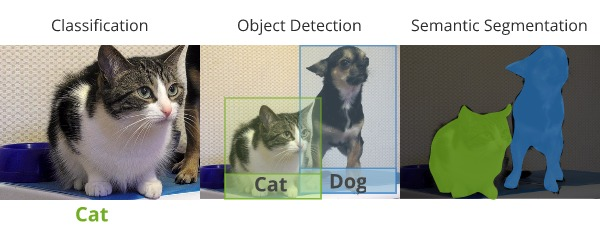
\includegraphics[width=0.7\linewidth]{images/classification_detection_segmentaion_comparisons.jpeg}
	\caption{Image Classification,Object detection Semantic Segmentation.}
\end{figure}
\subsection{Object Detection}\label{s:patt-dtct}
The goal of object detection is to detect all instances of objects from a known
class, such as people, cars or faces in an image. Typically only a small number
of instances of the object are present in the image, but there is a very large
number of possible locations and scales at which they can occur and that need
to somehow be explored \cite{chavan2016object}.
Each detection is reported with some form of pose information. This could
be as simple as the location of the object, a location and scale, or the extent
of the object defined in terms of a bounding box. In other situations the pose
information is more detailed and contains the parameters of a linear or non-linear
transformation. For example a face detector may compute the locations of the
eyes, nose and mouth, in addition to the bounding box of the face. An example
of a vehicle and person detection that specifies the locations of certain parts is shown in
\fref{f:patt-dtct}. The pose could also be defined by a three-dimensional transformation
specifying the location of the object relative to the camera.
Object detection systems construct a model for an object class from a set of
training examples. In the case of a fixed rigid object only one example may be
needed, but more generally multiple training examples are necessary to capture
certain aspects of class variability.
\begin{figure}[H]
	\centering
	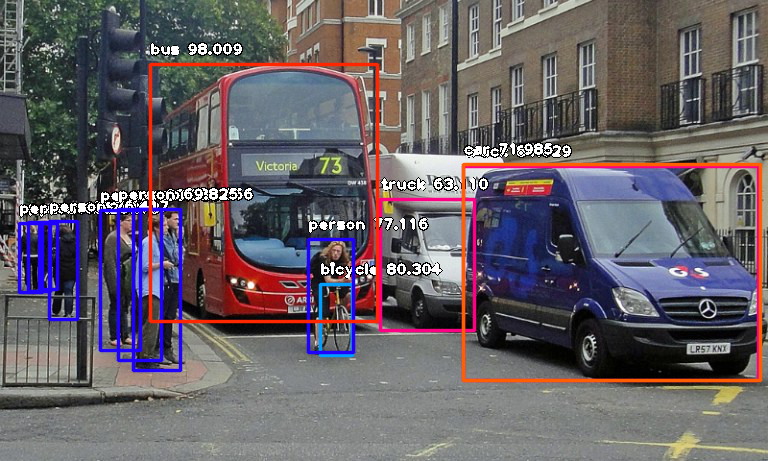
\includegraphics[width=0.5\linewidth]{images/object_det.jpeg}
	\caption{Object detection with bounding boxes.}
	\label{f:patt-dtct}
\end{figure}

Object detection methods fall into two major categories, generative (we use GAN\footnote{Generative Adversarial Network}) and discriminative (we use CNN). The first consists of a probability model for the image appearance on a given pose, together with a model for background, i.e. non-object images. The model parameters can be estimated from training data and the decisions are based on ratios of posterior probabilities \footnote{A posterior probability is the probability of assigning observations to groups given the data. A prior probability is the probability that an observation will fall into a group before you collect the data. For example, if you are classifying the buyers of a specific car, you might already know that 60\% of purchasers are male and 40\% are female. If you know or can estimate these probabilities, a discriminant analysis can use these prior probabilities in calculating the posterior probabilities. So a posterior probability uses known data to predict the probability the object will fall in that specific class}.
The second typically builds a classifier that can discriminate between images (or sub-images) containing the object and those not containing the object. The parameters of the classifier are selected to minimize mistakes on the training data, often with a regularization bias to avoid overfitting [\fref{f:overfitting}]. Other distinctions among detection algorithms have to do with the computational tools used to scan the entire image or search over possible poses, the type of image representation with which the models are constructed, and what type and how much training data is required to build a model.	

All the nets that preceded \maskrcnn only did Object Detection, as described in \sref{s:nnevo}.




\subsection{Semantic Segmentation}\label{s:patt-sema}
Segmentation is essential for image analysis tasks. Semantic segmentation describes the process of associating each pixel of an image with a class label, (such as flower, person, road, sky, ocean, or car).
Semantic image segmentation can be applied effectively to any task that involves the segmentation of visual information. Examples include road segmentation for autonomous vehicles, medical image segmentation, scene segmentation for robot perception, and in image editing tools. Whilst currently available systems provide accurate object recognition, they are unable to delineate the boundaries between objects with the same accuracy.

Oxford researchers have developed a novel neural network component for semantic segmentation that enhances the ability to recognise and delineate objects. This invention can be applied to improve any situation requiring the segmentation of visual information.

Semantic image segmentation plays a crucial role in image understanding, allowing a computer to recognise objects in images. Recognition and delineation of objects is achieved through classification of each pixel in an image. Such processes have a wide range of applications in computer vision, in diverse and growing fields such as vehicle autonomy and medical imaging.

The previous state-of-the-art image segmentation systems used Fully Convolutional Neural Network (FCNN) components, which offer excellent accuracy in recognising objects. Whilst this development represented a significant improvement in semantic segmentation, these networks do not perform well in delineating object boundaries.
\begin{figure}[H]
	\centering
	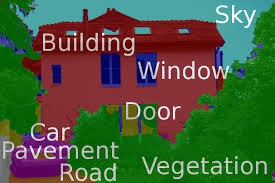
\includegraphics[width=0.5\linewidth]{images/semantic.jpg}
	\caption{Image with semantic segmentation.}
\end{figure}
Examples include, but are not limited to, road segmentation for autonomous vehicles, medical image segmentation, scene segmentation for robot perception and image editing tools.


\subsection{Instance Segmentation}\label{s:patt-insta}
Instance segmentation is one step ahead of semantic segmentation wherein along with pixel level classification, we expect the computer to classify each instance of a class separately. For example in the image above there are 3 people, technically 3 instances of the class “Person”. All the 3 are classified separately (in a different color). But semantic segmentation does not differentiate between the instances of a particular class.
\begin{figure}[H]
	\centering
	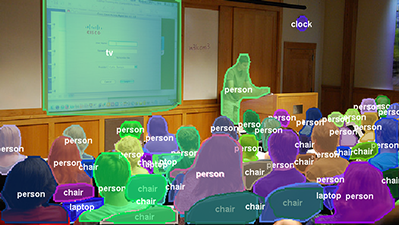
\includegraphics[width=0.5\linewidth]{images/instance.png}
	\caption{Image with instance segmentation.}
\end{figure}

That is what \maskrcnn does and is the best at, and why we chose it to pursue apparel recognition in real world images.



% ------------------------------------------------------------------
\section{NN evolution for Object Detection}\label{s:nnevo}
% ------------------------------------------------------------------

\subsection{Introduction}\label{s:nnevo-intro}

Images and videos are collected everyday by different sources. Recognizing objects, segmenting localizing and classifying them has been a major area of interest in computer vision. 

After having explained the basic features of Neural Networks [\sref{s:perc}] and CNNs [\sref{s:cnn-structure}] and having understood the task we're confronting with [Object Detection, \sref{s:patt-dtct}], we are ready to dive into how the algorithms for solving this problem have evolved in the last decades.

\subsection{Convolutional Neural Network}\label{s:nnevo-cnn}

Just as Convolutional Neural Network (CNN) is traced to the Fukushima’s \emph{ “neocognitron”} \cite{fukushima1980neocognitron}, a hierarchical and shift-invariant model for pattern recognition, the use of CNN for region-based identification (R-CNN)\cite{Girshick_2014} can also be traced back to the same.  After CNN was considered inelegant in the 1990s due to the rise of support vector machine (SVM, \fref{fig:svm}), in 2012 it was revitalize by Krizhevsky et al. \cite{krizhevsky2012imagenet} by demonstrating a valuable improvement in image classification accuracy on the ImageNet Large Scale Visual Recognition Challenge (ILSVRC), explained in \ref{s:imagenet}, and included new mechanisms to CNN like rectified linear unit (ReLU) and, dropout regularization. You can check out the tecnical details on how a CNN works in \sref{s:cnn-structure}.

\subsection{Region-based CNN}\label{s:nnevo-rcnn}

To perform object detection with CNN and in attempt to bridge the gap between image segmentation and object detection two issues were fixed by R.Girshick et al \cite{Girshick_2014}. First was the localization of objects with a Deep Network and training a high-capacity model with only a small quantity of annotated detection data. Use of a sliding-window detector was proposed for the localization of object but was not preferred because it can only work for one object detection and all objects in an image have to have a common aspect ratio for its use in multiple object detection. Instead the localization problem was solved by operating within the “recognition using regions” paradigm.

The Region-based Convolutional Neural Network (R-CNN) is relatively simple. First, we propose some regions of an image which contain objects. We feed these regions into a CNN, and then we use an SVM to classify the outputs for each class.

\begin{center}
	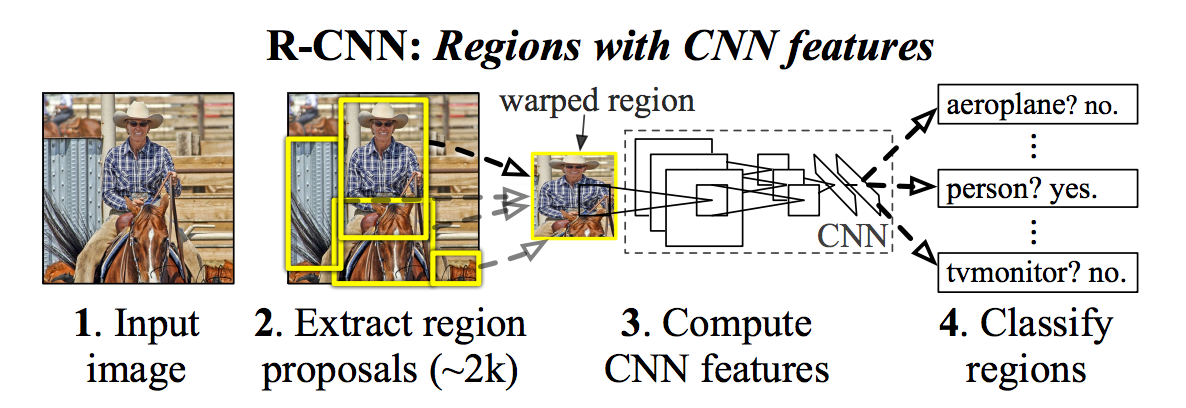
\includegraphics[scale=0.3]{images/rcnn.png}
\end{center}

If we wish to have a CNN classify objects in images, we need to feed in a region of the image to the CNN. Of course, the question becomes: How do we know which regions to feed into a network? We cannot possibly try every single possible region of an image; there are too many combinations. We must have a way to propose regions which are likely to contain objects.

\begin{figure}[H]
	\centering
	\begin{minipage}{0.45\textwidth}
		\centering
		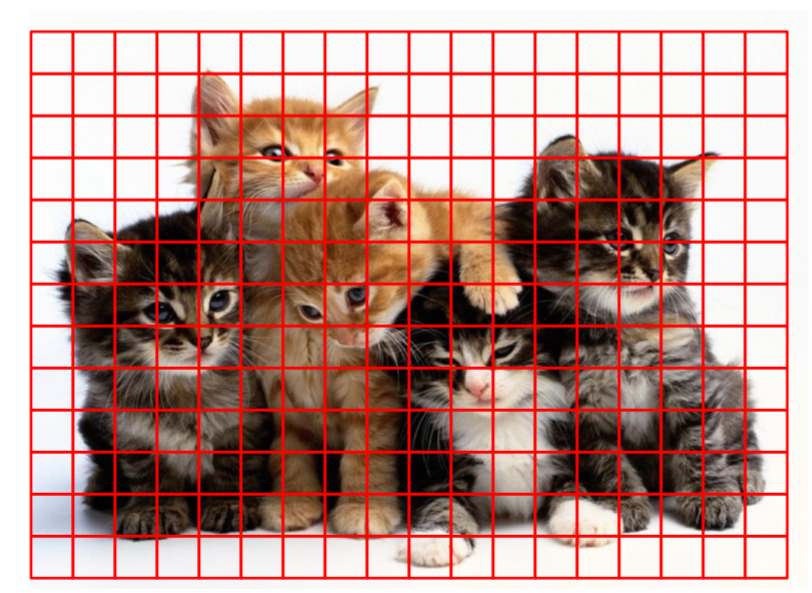
\includegraphics[width=0.66\textwidth]{images/search.PNG} % first
		\caption{Too many regions!}
		\label{f:regionscnn}
		%figure itself
	\end{minipage}\hfill
	\begin{minipage}{0.45\textwidth}
		\centering
		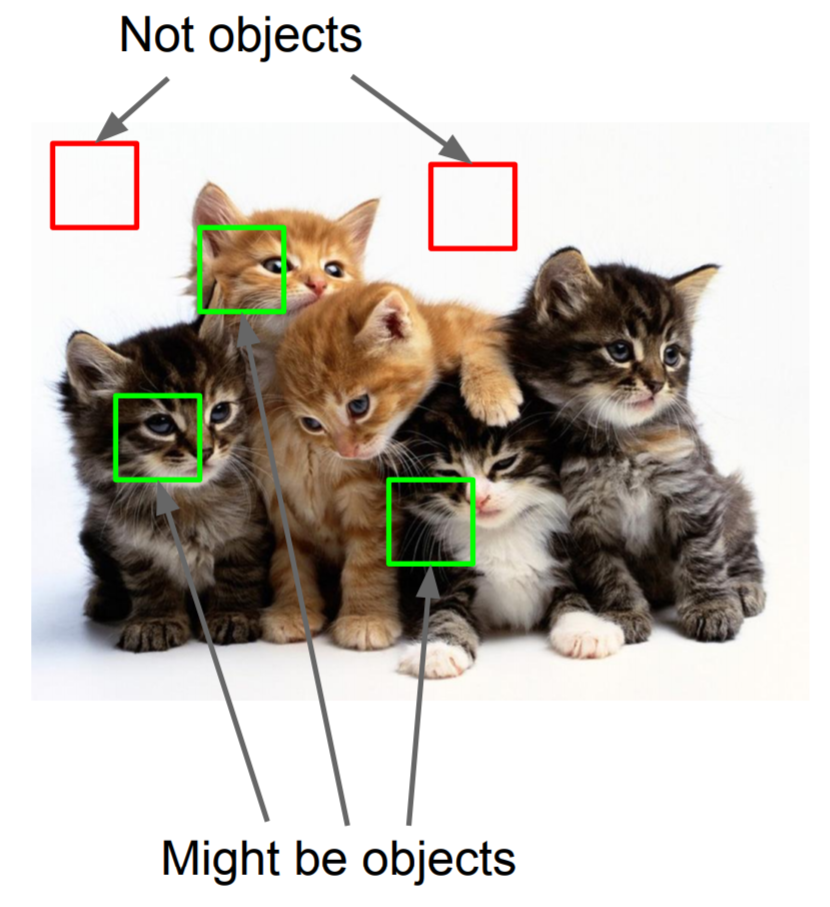
\includegraphics[width=0.66\textwidth]{images/region.PNG} % second figure itself
	\end{minipage}
\end{figure}

R-CNN is agnostic to the region proposal algorithm. The original R-CNN uses the Selective Search algorithm. Since selective search, various region proposal methods have been developed.

Selective Search detects image segments to propose regions. It uses the segments it finds to identify the containing boxes, which will be used by R-CNN as regions.

\begin{figure}[H]
	\centering
	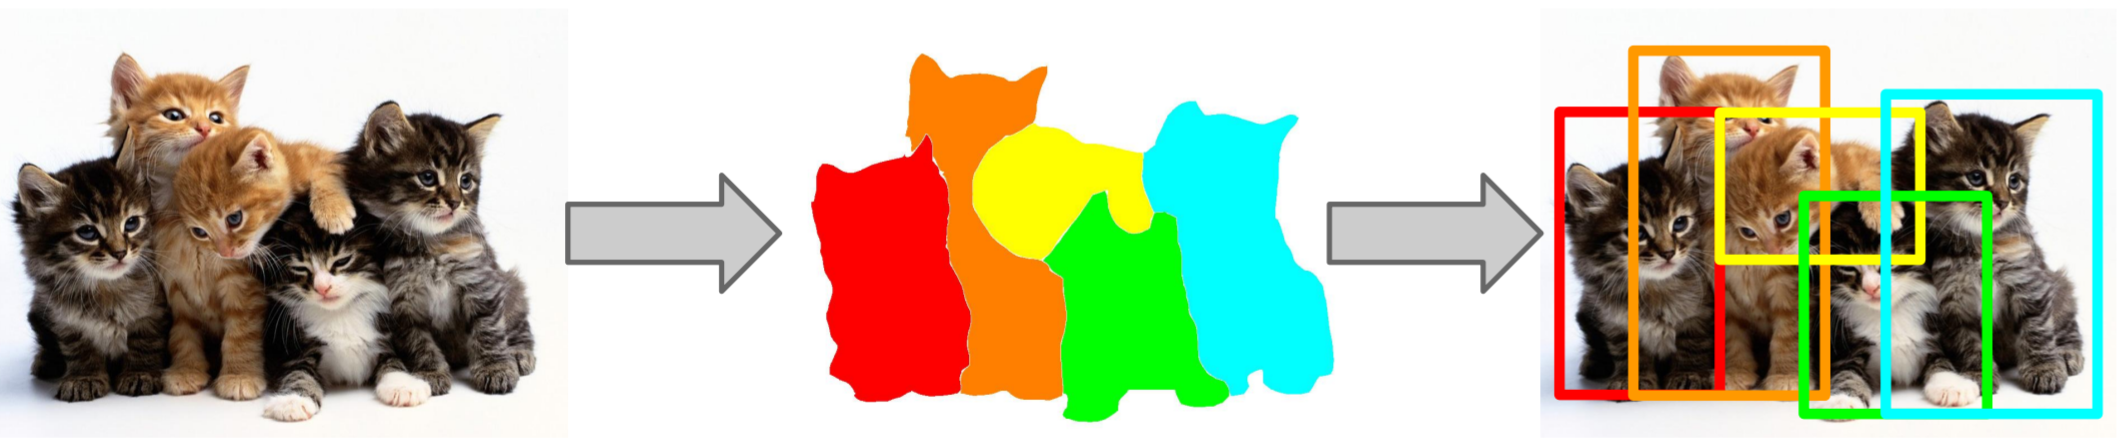
\includegraphics[scale=0.4]{images/segment.PNG}
	\caption{Using segments to define regions}
	\label{f:segment}
\end{figure}

\subsection{Fast R-CNN}\label{s:nnevo-fastrcnn}

Fast R-CNN was introduced in 2015 by Girshick \cite{Girshick_2015}. A single-stage training algorithm that jointly learns to classify object proposals and refine their spatial locations was demonstrated.

\begin{figure}[H]
	\centering
	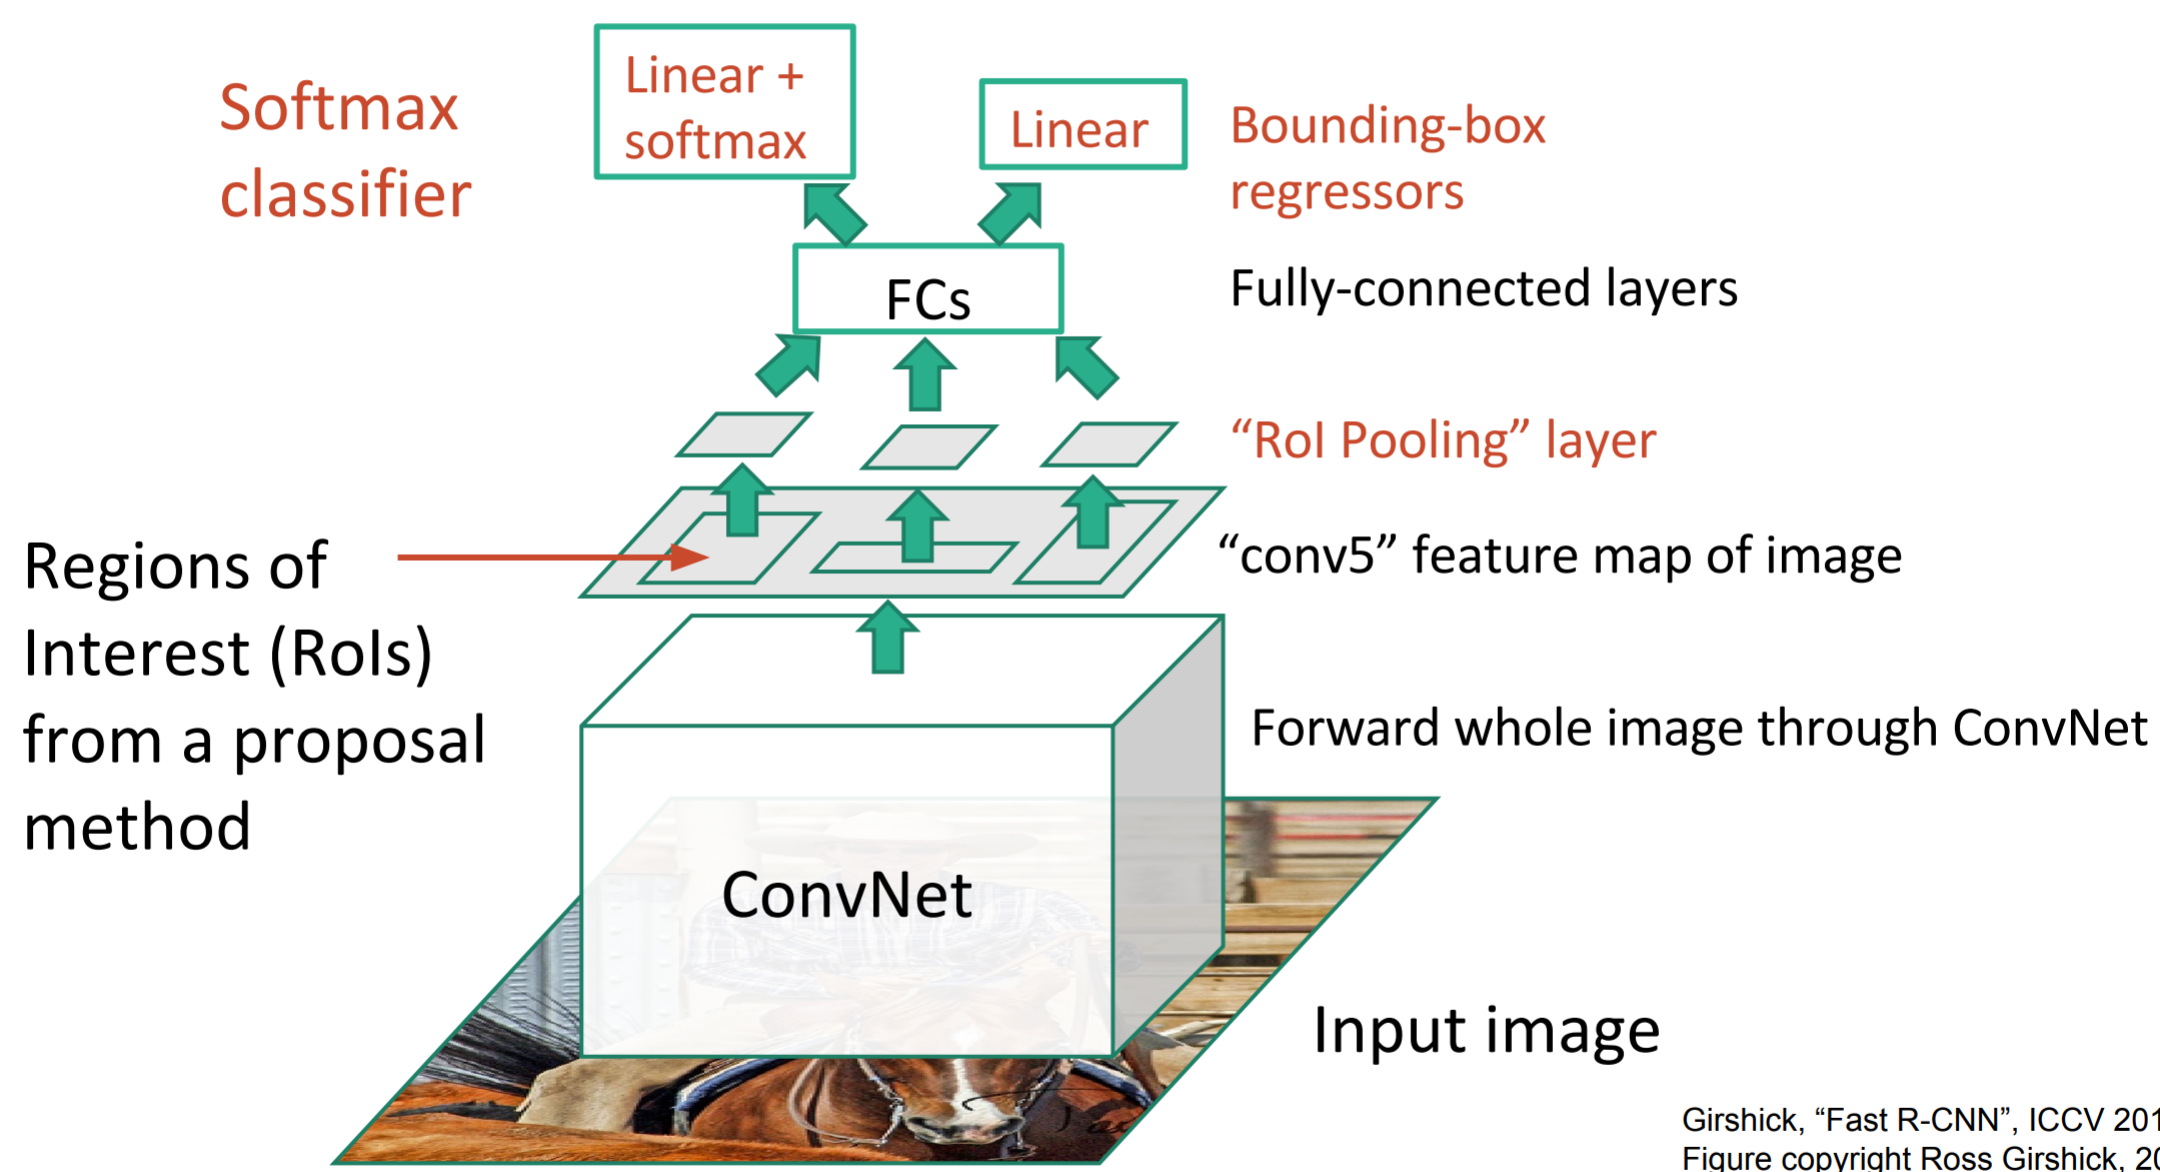
\includegraphics[scale=0.35]{images/fastrcnn.PNG}
	\caption{Fast R-CNN Architecture}
	\label{f:fastrcnn}
\end{figure}

Fast R-CNN, instead of running the CNN for each region, runs it just a single time. And then takes the regions from the convolutional feature map (the output of a filter applied to the previous layer).

This tackled the problem of complexity that arises in other deep ConvNets, caused by the multi-stage pipelines that are slow. The slow nature is due to the fact that detection requires accurate localization of objects that creates the challenge of that many proposals (candidate object locations) must be processed and these proposals provides only rough localization that must be refined to achieve precise localization. Fast R-CNN is 9 X faster than R-CNN \cite{Girshick_2014} and 3 X faster than SPPnet \cite{he2015spatial}. R-CNN was sped up by \emph{Spatial pyramid pooling networks (SPPnets)}\cite{he2015spatial} by sharing computation. A convolutional feature map for the entire input image was computed by SPPnet method. After which it then classifies each object proposal using a feature vector extracted from the shared feature map. 

\fref{f:fast-rcnn-arch} below makes it clear that Fast R-CNN proposes regions of interest ``RoI" from the input image. These are generated using a region proposal algorithm (e.g. Selective Search), just like they were in R-CNN.

\begin{figure}[H]
	\centering
	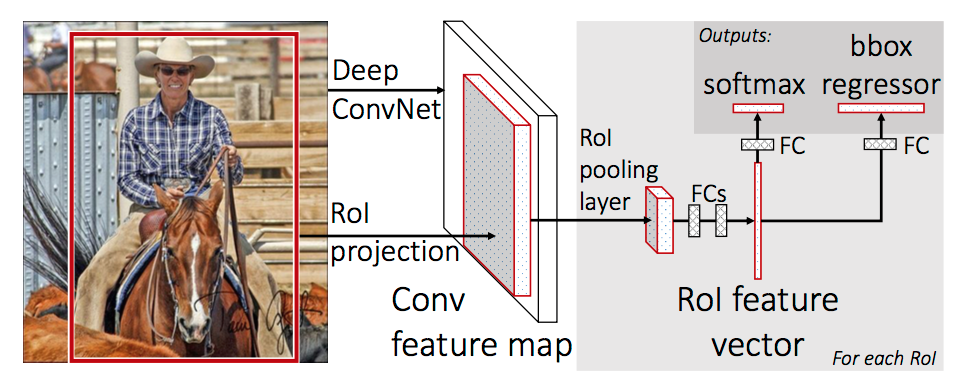
\includegraphics[scale=0.55]{images/fast-rcnn-arch.png}
	\caption{Fast R-CNN RoI Projection}
	\label{f:fast-rcnn-arch}
\end{figure}

However, in Fast R-CNN, as \fref{f:fastrcnn} shows, these regions of interest are then projected onto the convolutional feature map. This allows us to re-use the expensive convolutional computation. We take crops from this feature map and run them through the rest of the network. The question then becomes: how exactly do we \textit{project} a region of the input image onto a region of the convolutional feature map?

The SPPNet paper (``Spatial Pyramid Pooling in Deep Convolutional
Networks for Visual Recognition" by He et al.)~\cite{he2015spatial}, which came out between R-CNN and Fast R-CNN, first introduced the idea of RoI projection.

RoI Projections are of course different from cropping an image, so here comes RoI Pooling, which is described in \sref{s:roi-pooling}.

SPPnet also has obvious pitfalls. It is a multi-stage pipeline similar to R-CNN that involves extracting features, refining a network with log loss, training SVMs, and lastly fitting bounding-box regressors. Features are also written to disk. But unlike R-CNN, the refining algorithm demonstrated in SPPnet cannot update the convolutional layers that precede the spatial pyramid pooling. This constraint limits the accuracy of very deep networks.

Even though SVMs worked better than Softmax [\sref{s:softmax}] in R-CNN, the opposite is true for Fast R-CNN. This was demonstrated only empirically, as per \tref{t:fastrcnn-svmvssoftmax}

\begin{table}[H]
	\centering
	\begin{tabular}{c c c c} 
		\hline
		Method (VGG16) & Classifier & VOC07 \\ [0.5ex] 
		\hline
		R-CNN & Post-hoc SVM & 66.0\% \\
		Fast R-CNN & Post-hoc SVM & 66.8\% \\
		Fast R-CNN & Softmax & 66.9\% \\
		\hline
	\end{tabular}
	\caption{SVM vs Softmax for training the probability distribution for each RoI}
	\label{t:fastrcnn-svmvssoftmax}
\end{table}

Also, Fast R-CNN greatly improves upon the speed of R-CNN -- so much so that the region proposal algorithm takes the vast majority of time during testing, as shown below in \fref{f:chart}.

\begin{figure}[H]
	\centering
	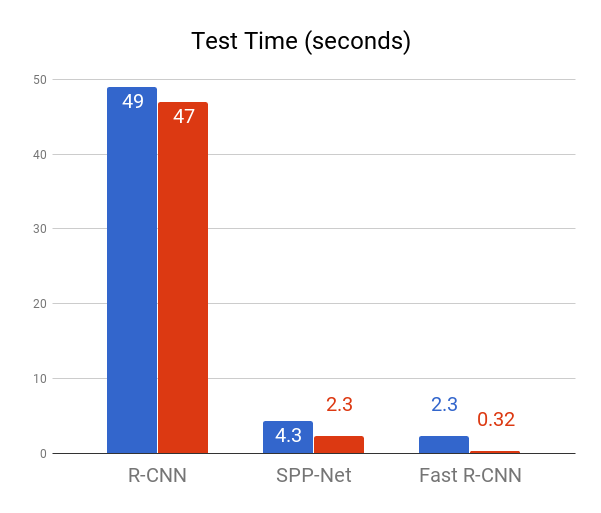
\includegraphics[width=0.75\textwidth]{images/chart.png} %second
	\caption{Training Time R-CNN, SPPNet and Fast R-CNN. Blue bars include region proposal algorithm.}
	\label{f:chart}
\end{figure}

Faster R-CNN sets out to solve the problem of slow region proposal!

\subsection{Faster R-CNN}\label{s:nnevo-fasterrcnn}

Additional efforts were made to reduce the running time of deep ConvNets for object detection and segmentation. Regional proposal computation is the root of this expensive running time in detection networks. Even the fast EdgeBoxes algorithm takes 0.3 seconds, as in \fref{f:table} below.

\begin{figure}[H]
	\centering
	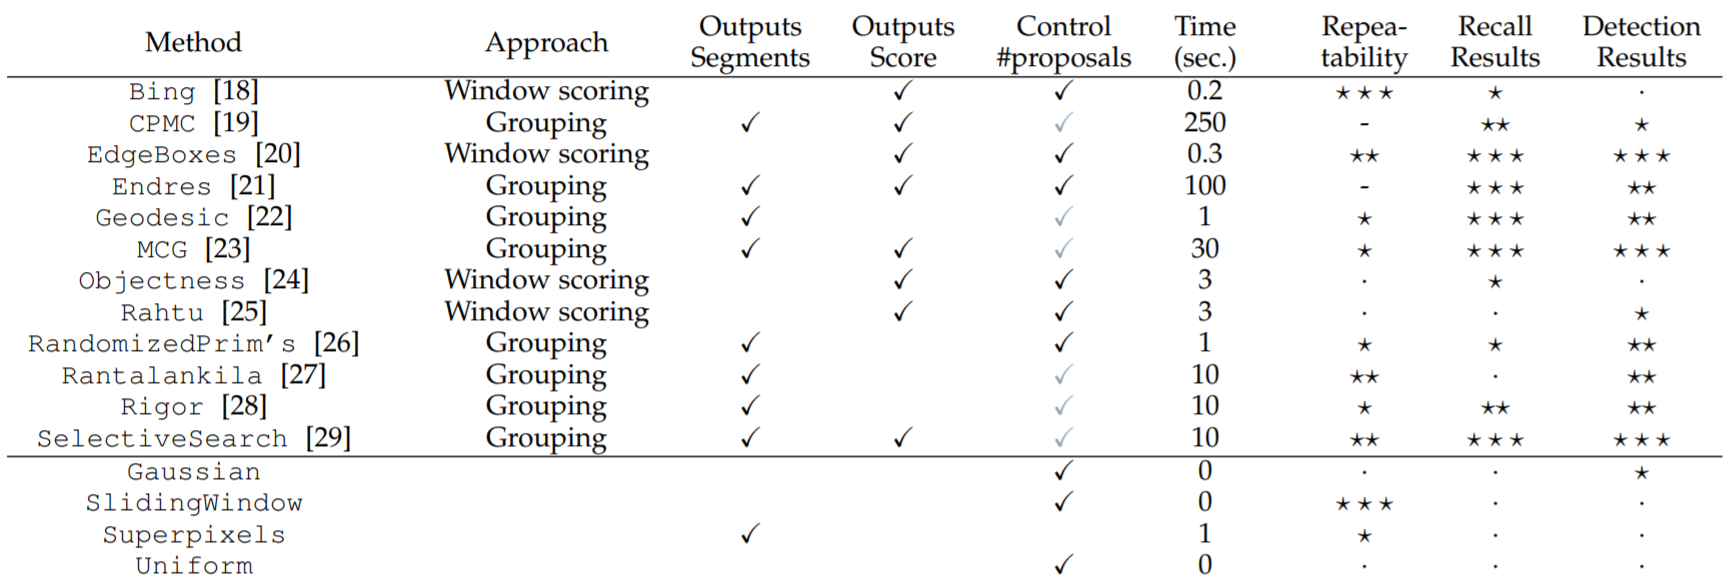
\includegraphics[scale=0.5]{images/table.PNG}
	\caption{Region Proposal Algorithms comparison.}
	\label{f:table}
\end{figure}

A fully convolutional network that simultaneously predicts object bounds and objectness scores at each position called \emph{ Region Proposal Network (RPN) }was developed by Ren et al \cite{ren2015faster}. RPN shares full-image convolutional features with the detection network, thus permitting virtually cost-free region proposals and it is trained end-to-end to generate high-quality region proposals.

To put it simply, it leverages the filter map output we used in Fast R-CNN to propose regions. This time, though, the proposing algorithm is a neural net that learns to predict the more plausible regions, and not a fixed algorithm such as the ones above in \fref{f:chart}.
After all, if convolutions are good enough for classification and bounding-box regression, why wouldn't they work for region proposals as well?

Integrating RPN and Fast R-CNN into a unit network by sharing their convolutional features results to Faster R-CNN.

% TODO RPN in detail

Anchor boxes that acts as reference at multiple scales and aspect ratios were introduced in Faster R-CNN instead of the pyramids of filters used in earlier methods. RPNs are developed to coherently speculate region proposals with an extensive range of scales and aspect ratios.

Changing the architecture of the pyramids of filter to a top-down architecture with lateral connections improved the efficiency of this pyramids \cite{lin2017feature}. This is applied in building high-level semantic feature maps at all scales. This new architecture is called \emph{ Feature Pyramid Network (FPN)} \cite{lin2017feature}, shown in comparison with ResNet in \sref{s:maskrcnn-maskhead}. In various applications and uses it displayed a notable improvement as a generic feature extractor. When used in a Faster R-CNN it achieved results that supersedes that of Faster R-CNN alone. 

\subsection{Mask R-CNN}\label{s:nnevo-maskrcnn}

In order to generate a high-quality segmentation mask for object instances in an image, \maskrcnn was developed \cite{He_2017}. \maskrcnn adds another branch to the Faster R-CNN. In addition to the bounding box recognition system a branch for predicting an object mask in parallel was added. It affixes only a bijou overhead to Faster R-CNN. 

This allows for our task: Instance Segmentation, \sref{s:maskrcnn}, in which I'll describe in more detail the features of \maskrcnn.


\section{Instance Segmentation}\label{s:maskrcnn}

Instance Segmentation is one of the most difficult image-based computer vision tasks. It combines elements of semantic segmentation (pixel-level classification) and object detection (instance recognition). Essentially, at every pixel, we wish to classify not only the type of object (or background) the pixel is part of, but also determine which instance the pixel is part of, as described in \sref{s:patt}

\begin{figure}[H]
	\centering
	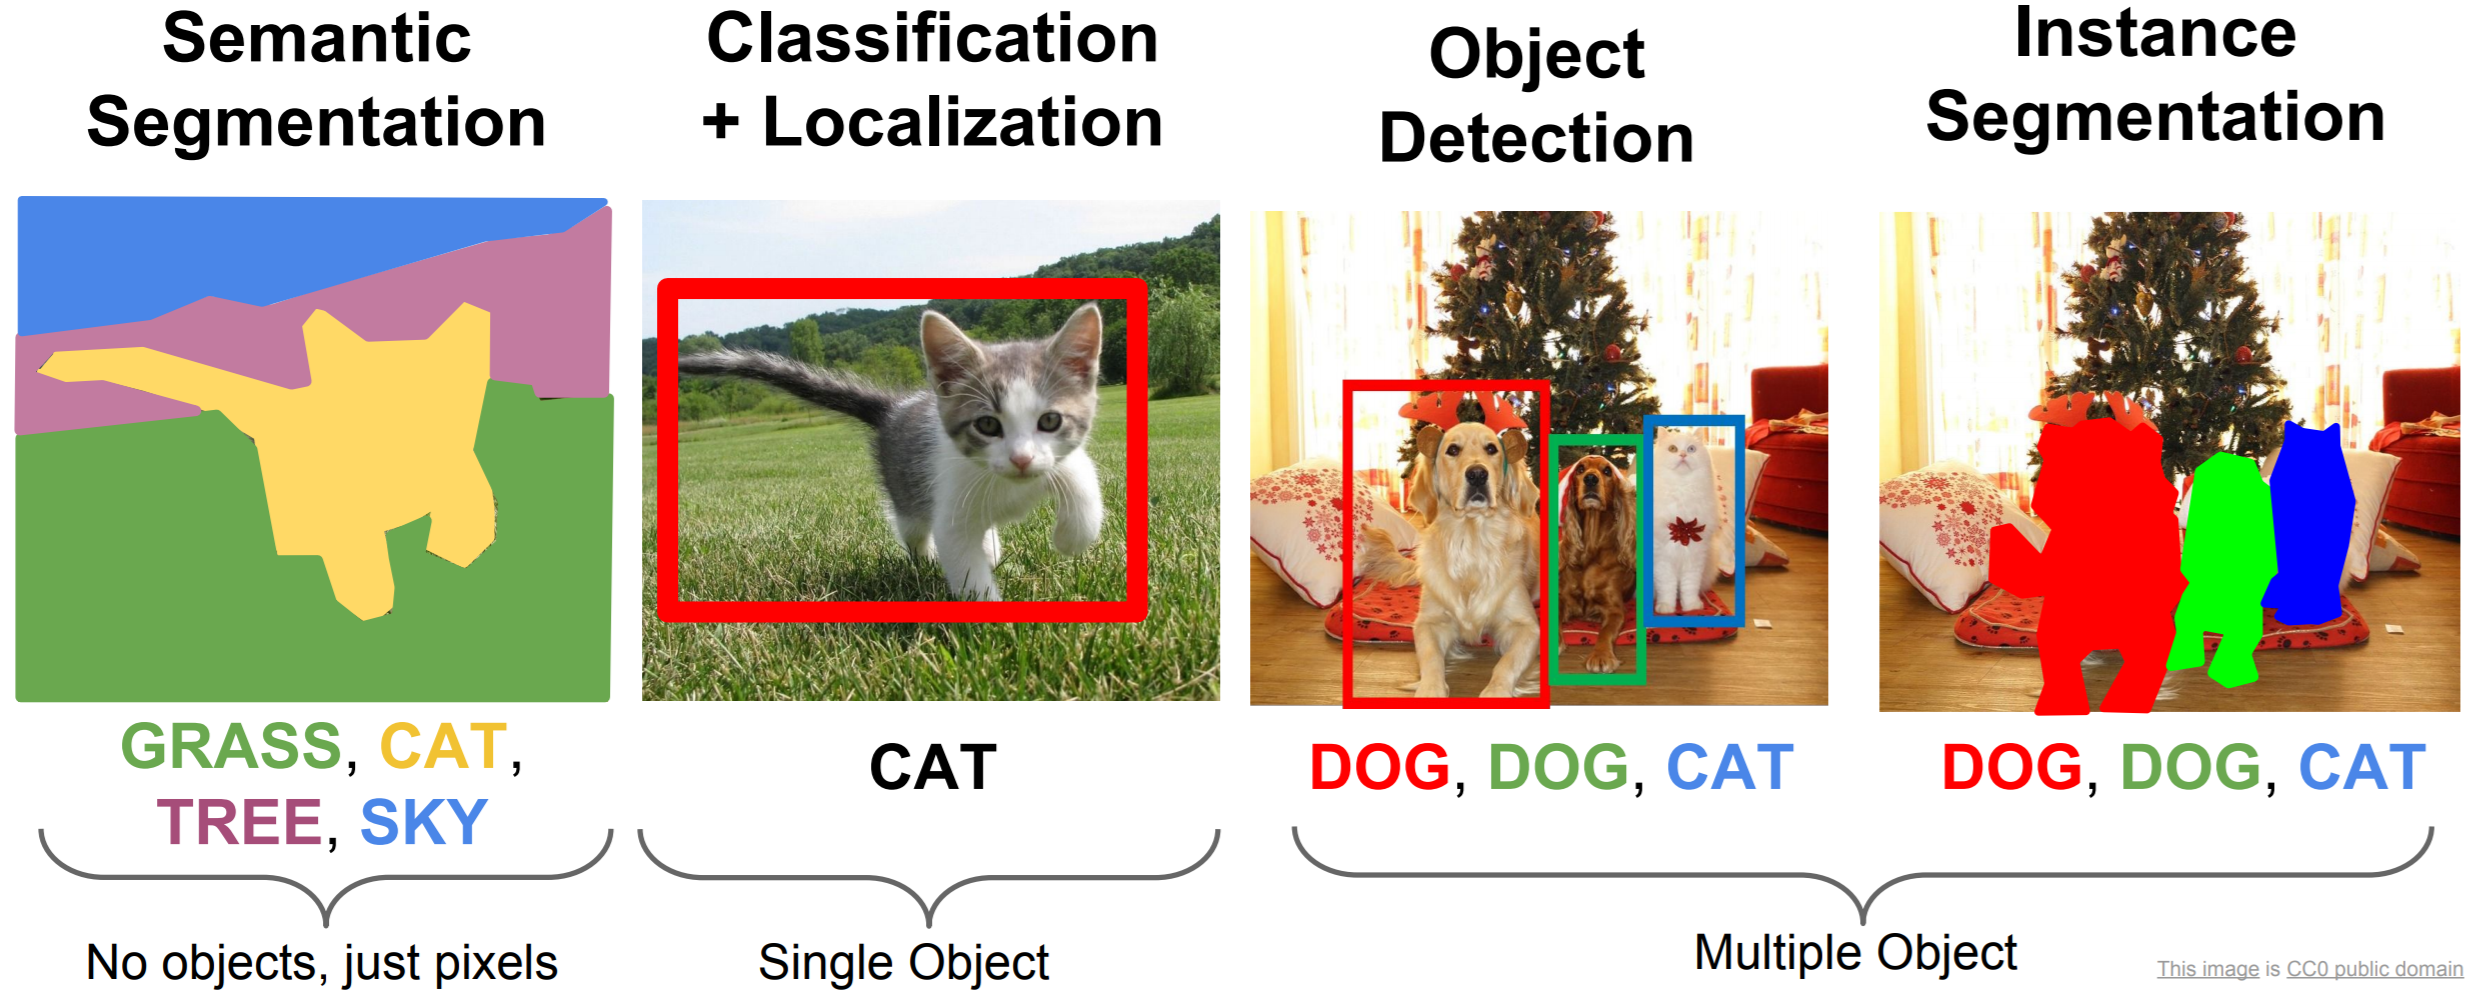
\includegraphics[scale=0.3]{images/tasks.PNG}
	\caption{Pattern recognition tasks.\newline Source: Fei-Fei Li Stanford Course -- Detection And Segmentation}
	\label{f:tasks}
\end{figure}

Not unsurprisingly, instance segmentation networks rely heavily on existing object detection networks. \maskrcnn modifies the Faster R-CNN architecture and adapts it for instance segmentation with minimal overhead. \maskrcnn is the current leader in instance segmentation performance.

A previous ``fully convolutional instance segmentation" (FCIS) solution, which performed segmentation, classification, and bounding-box regression simultaneously, although very fast, exhibited low segmentation accuracy, especially on overlapping objects. \maskrcnn therefore takes a different approach, \textit{decoupling} segmentation from classification and bounding-box regression. \maskrcnn thus adds a separate mask ``head" to the Faster R-CNN network. This is shown in the diagram below.

The mask ``head" is simply a small fully convolutional network that outputs an $m\times m$ mask for each region proposal. We use a fully convolutional network rather than fully connected layers so we do not lose spatial information. A fully convolutional solution requires fewer parameters than previous fully connected solutions while simultaneously increasing accuracy.

The two diagrams at the bottom of \fref{f:fastermaskrcnn} show a different visualization of Faster R-CNN and \maskrcnn. Besides the additional ``mask" head of \maskrcnn, we can see that RoIAlign replaces RoI Pooling and is described in \sref{s:roi-align}

\begin{figure}[H]
	\centering
	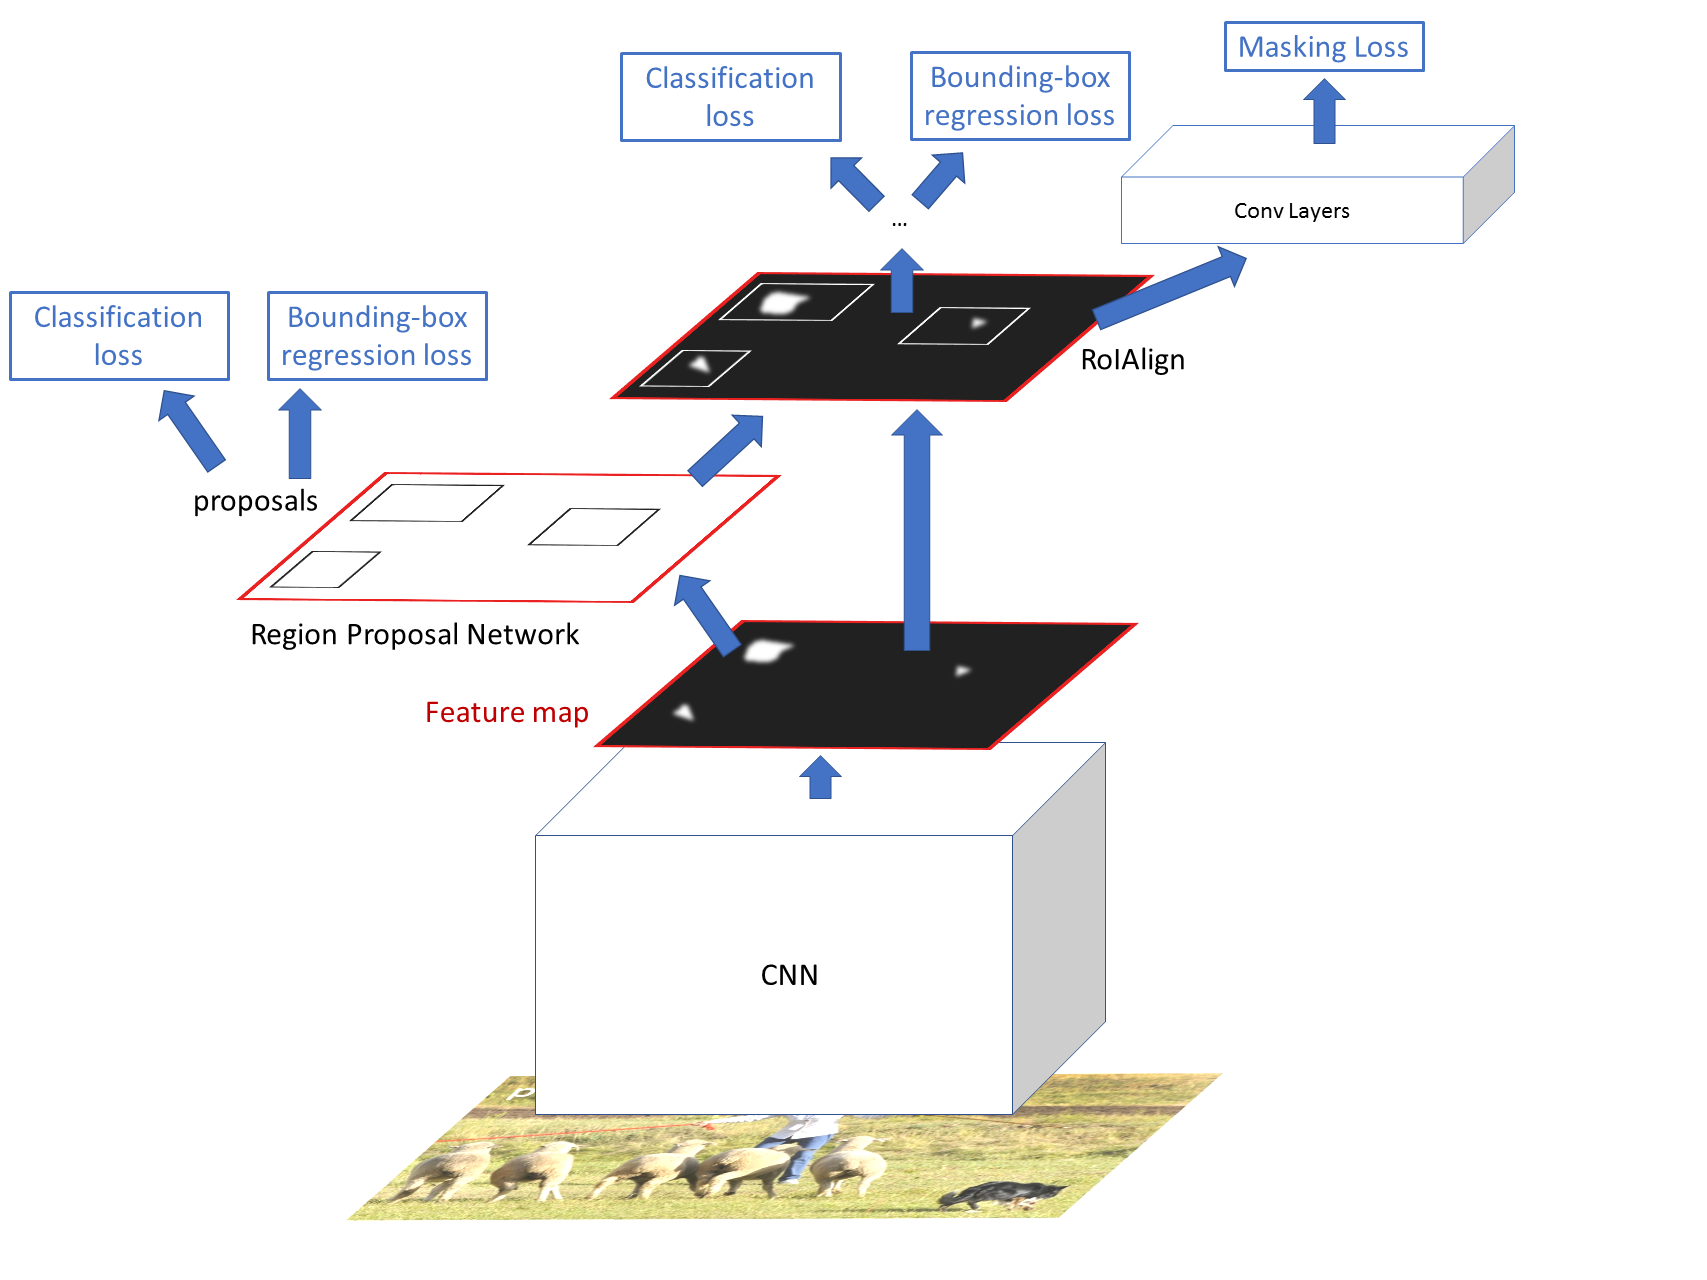
\includegraphics[scale=0.36]{images/masknetwork.png}

	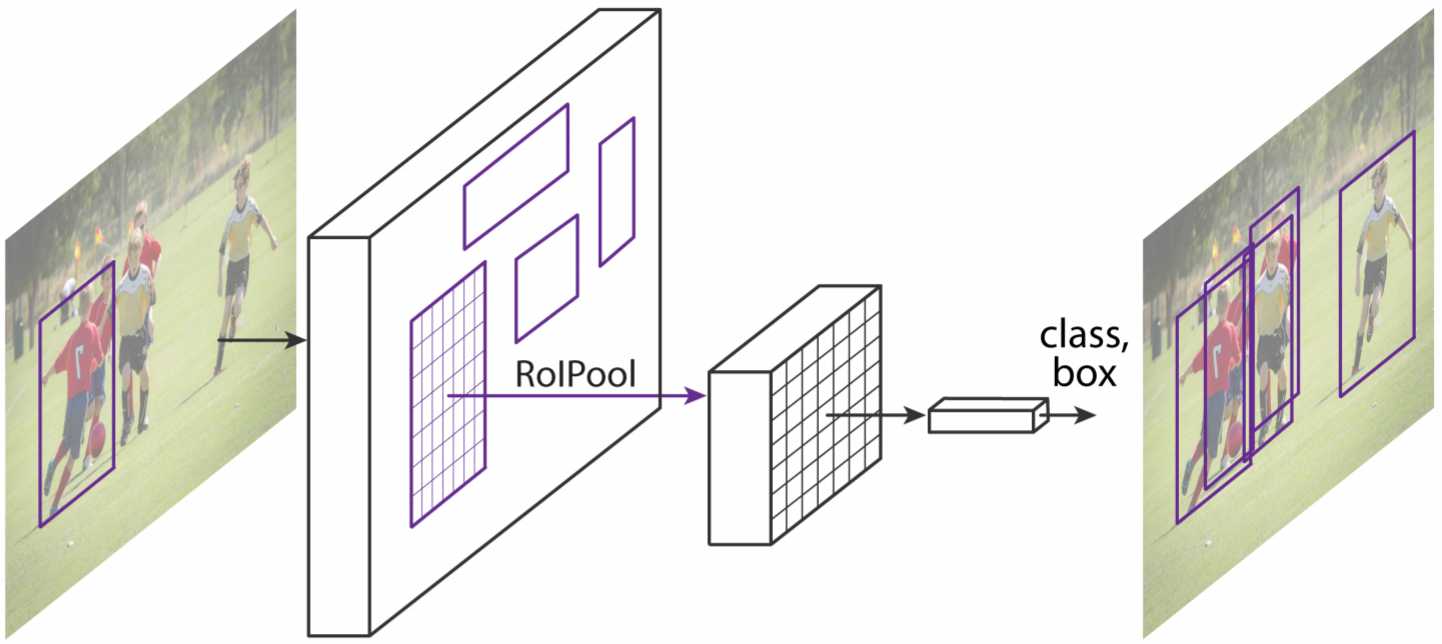
\includegraphics[scale=0.45]{images/fasterrcnnvs.PNG}

	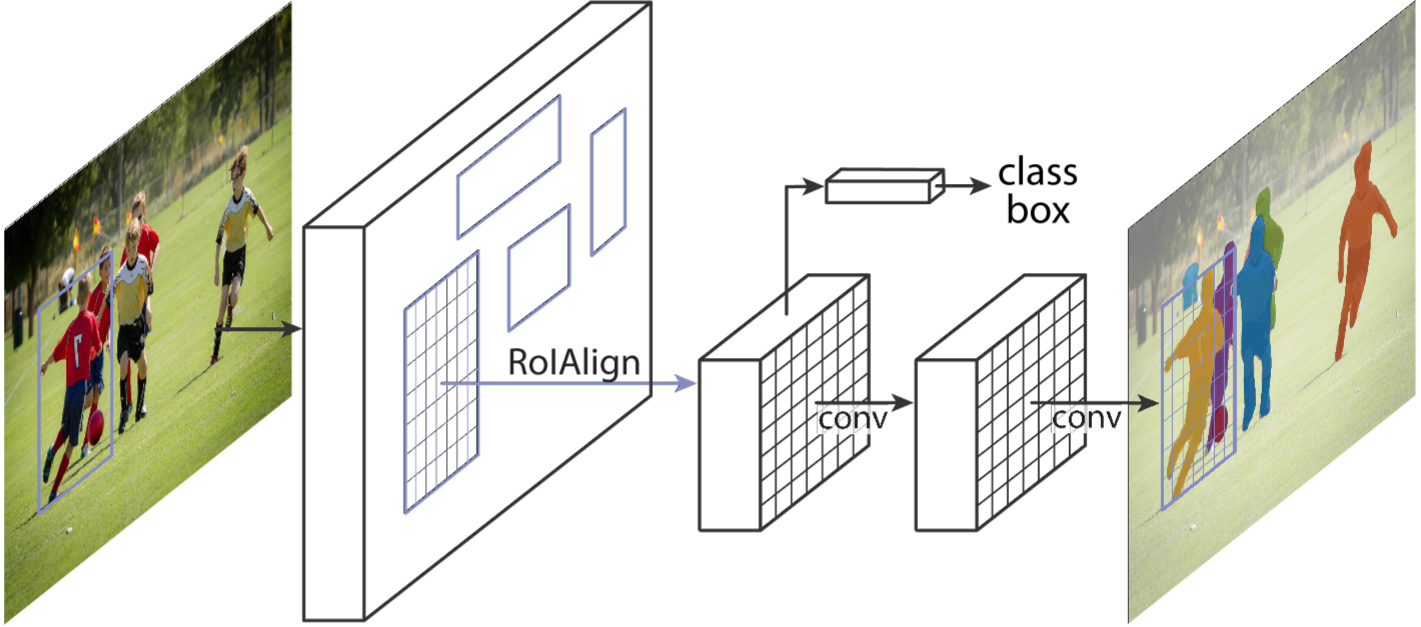
\includegraphics[scale=0.45]{images/maskrcnn.PNG}

	\caption{Faster R-CNN vs \maskrcnn}
	\label{f:fastermaskrcnn}
\end{figure}

The output of RoI Align is then passed through the fully connected layers for bounding-box regression and classification, and through the small Fully Convolutional Network (FCN) that makes up the masking head.

\subsection{Mask Head}\label{s:maskrcnn-maskhead}
Depending on the network backbone, the mask head differs for \maskrcnn. Below is a look at the two different heads. Both are trivial FCNs.

\begin{figure}[H]
	\centering
	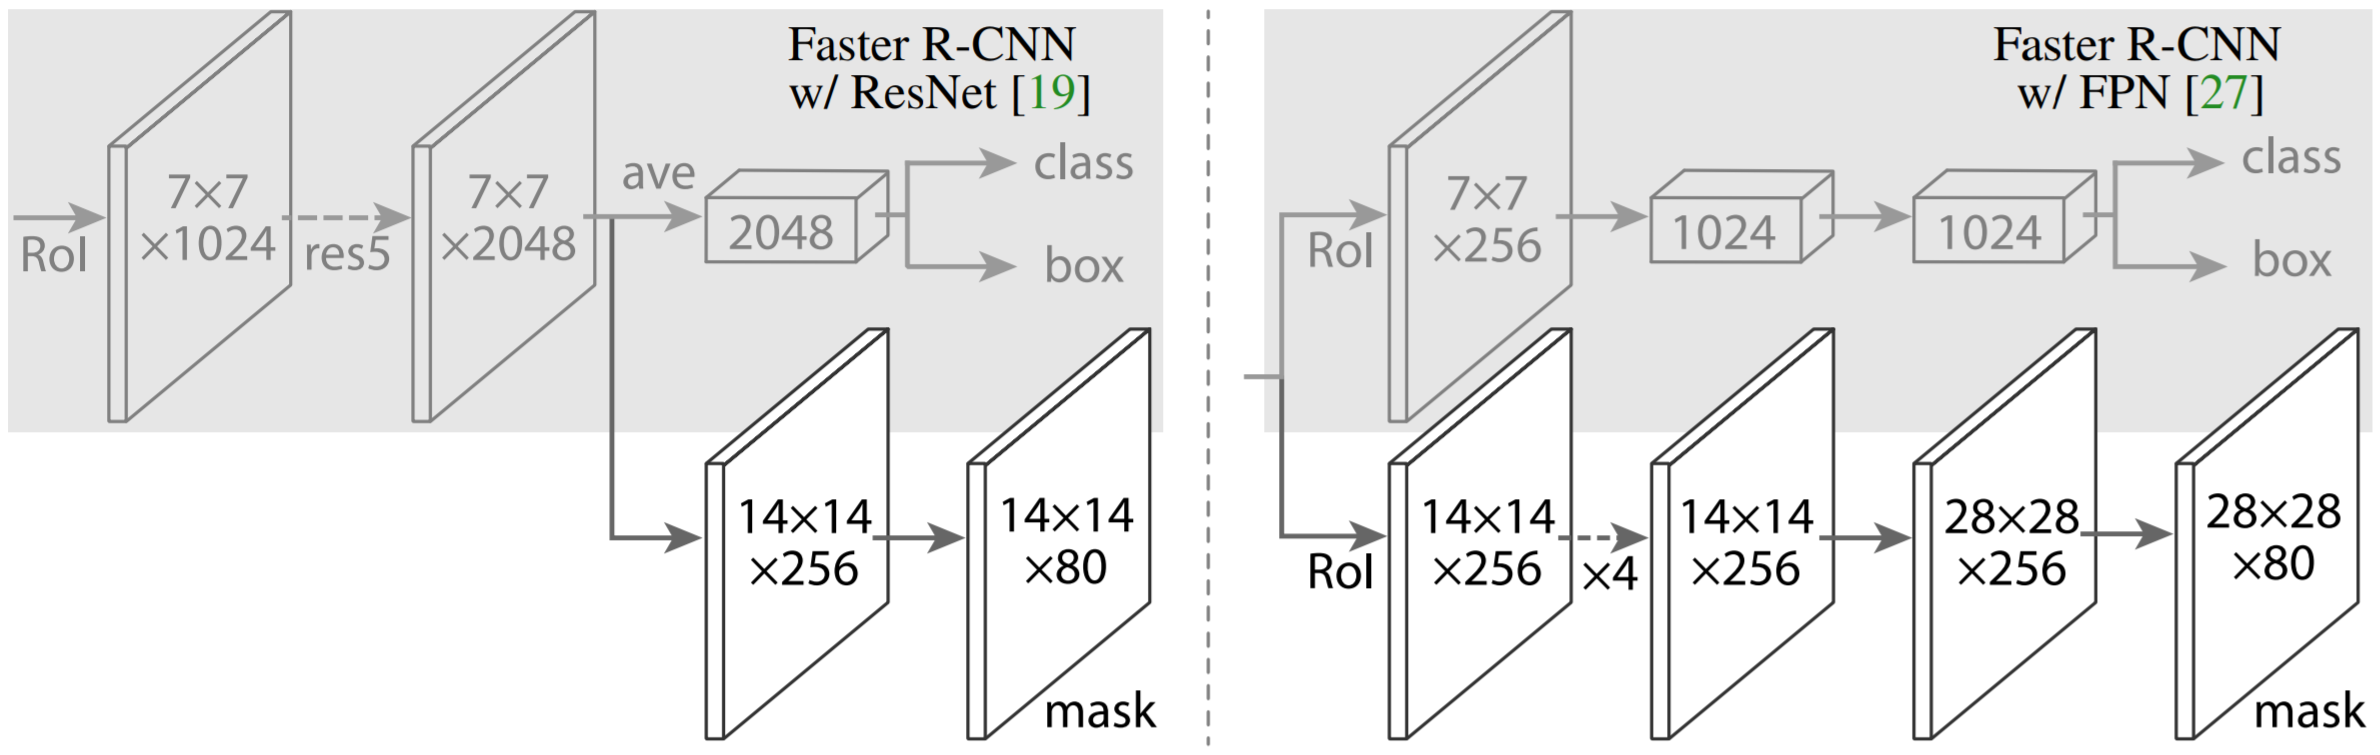
\includegraphics[scale=0.3]{images/backbones.PNG}
	\caption{Comparison between Faster R-CNN with ResNet or FPN backbone}
\end{figure}

In the diagram above, FPN stands for ``Feature Pyramid Network", introduced in \sref{s:nnevo-fasterrcnn}. ResNet, meanwhile, is described in \sref{s:imagenet-resnet}.

There are a few important things to know about this mask head. First, like we said earlier, our output is an $m\times m$ mask. However, the authors found it beneficial to have binary masks. In other words, we predict $K$ $m\times m$ masks for each RoI, where $K$ is the number of classes. One mask per class. Thus, the mask branch has a $Km^2$-dimensional output for each region of interest.

Our loss function is now different. Previously, we had $L = L_{boundingbox} + L_{classification}$. We've covered the details of classification and bounding-box loss in our object detection, for both the region proposal network (RPN) and the network itself. For \maskrcnn, we add another loss, $L_{mask}$. For some region $r$, if the ground truth class is $k$, we apply a per-pixel sigmoid on \textit{only} the $k$th mask. This allows us to define $L_{mask}$ as the average binary cross-entropy loss. Thus, the masks for classes that don't correspond to the ground truth aren't calculated. (remember, we have one mask per class for every region).

By computing one mask per class, we are \textit{decoupling} classification and segmentation. We simply don't care what class the object is when we segment it. Previous practices, like FCNs for semantic segmentation, use multi-class cross-entropy losses and per-pixel softmax. These allows for competition between classes, which \maskrcnn eliminates.

\subsection{Training and Testing}
When training, \maskrcnn shares similarities with its object detection cousins. Hyperparameters were set to the same values. Positive RoIs have IoU, described in \fref{f:iou}, of at least 0.5 with the ground truth box. In addition, $L_{mask}$ is defined only on positive RoIs. The mask target is the intersection between an RoI and its associated ground-truth mask. 

At test time, after non-maximum supression is applied, the masking branch is applied on only the top 100 RoIs. If an region was classified into class $k$, we simply choose the $k$th mask. The mask is then resized to the size of the region of interest. By reducing segmentation computation to only 100 regions, we dramatically decrease the amount of overhead. In fact, \maskrcnn runs at 5 fps, compared to Faster R-CNN's 7 fps.

\subsection{Model Performance}
The \maskrcnn paper \cite{He_2017} not only provides evidence that their model outperforms all previous models, but also conducted various ablation experiments to show that RoIAlign [\sref{s:roi-align}], segmentation decoupling, and fully convolutional mask heads [\sref{s:maskrcnn-maskhead}] each individually improve accuracy. The results are shown in the tables below.


\begin{figure}[htbp]
	\centering
	\begin{minipage}{0.55\textwidth}
		\centering
		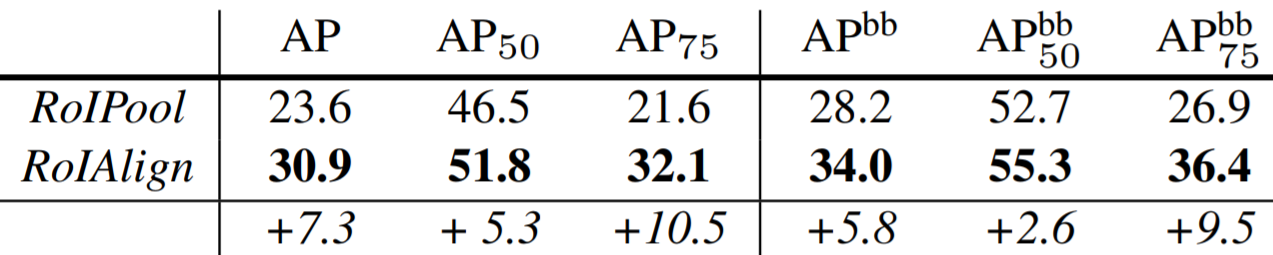
\includegraphics[width=1\textwidth]{images/moreroialigncomparison.PNG} % first
		%figure itself
	\end{minipage}\hfill
	\begin{minipage}{0.35\textwidth}
		\centering
		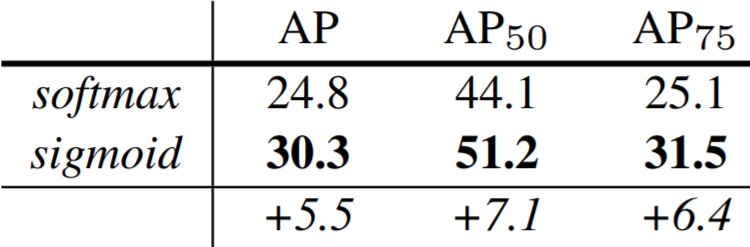
\includegraphics[width=1\textwidth]{images/binarymaskcomparison.PNG} %second
		%figure itself
	\end{minipage}
\end{figure}

\begin{center}
	\includegraphics[scale=0.4]{images/fcncomparison.PNG}
\end{center}

In addition, \maskrcnn performs better with a deeper backbone CNN. However, it should be noted that the 5 fps speed was achieved using the shallow ResNet-50 network as a backbone. (If you really want to call it “shallow")

\begin{center}
	\includegraphics[scale=0.4]{images/backbonecomparison.PNG}
\end{center}

The results on the COCO and Cityscapes benchmarks are shown below. \maskrcnn performs with state-of-the-art accuracy on both.
\begin{figure}[htbp]
	\centering
	\includegraphics[width=0.85\textwidth]{images/cocoresults.PNG} % first
	\caption{COCO results.}
\end{figure}
\begin{figure}[htbp]
	\centering
	\includegraphics[width=1\textwidth]{images/cityscapesresults.PNG} % first
	\caption{Cityscapes results.}
\end{figure}


\begin{figure}[H]
	\centering
	\begin{minipage}{0.35\textwidth}
		\centering
		\includegraphics[width=1\textwidth]{images/cocoexamples.PNG} % first
		%figure itself
	\end{minipage}\hfill
	\begin{minipage}{0.65\textwidth}
		\centering
		\includegraphics[width=1\textwidth]{images/cityscapes.PNG} %second
		%figure itself
	\end{minipage}
	\caption{Segmentation examples from COCO (left) and Cityscapes (right)}
	\label{f:maskrcnn-instancecity}
\end{figure}
\maskrcnn can also be used for human pose estimation.


\maskrcnn leaps ahead of the competition in terms of pure instance segmentation performance. However, no current instance segmentation method can achieve great results while operating in real-time (60 FPS). In the future, we look for networks which dramatically improve segmentation speed as well as accuracy.



% ------------------------------------------------------------------

 \chapter{Dataset}\label{s:ds}

\section{Introduction}\label{s:ds-intro}

As I explained in the Abstract, I chose \modanet after having looked at many others.

An interesting one I found, for example, was DeepFashion \cite{DeepFashion2}, but it didn't feature any footwear annotations unfortunately -- which were the main focus of the task I was given. It had over 800 thousand images though!

\begin{figure}[H]
	\centering
	\includegraphics[width=0.75\textwidth]{images/deepfashion2_bigbang}
	\caption{DeepFashion2 feature image.}
	\label{f:deepfashion2_bigbang}
\end{figure}

But what is a dataset? Simply speaking, a dataset is a collection of data that is usually useful for statistics / data analysis purposes. Many datasets today cannot be fully exploited due to our technology, but this is rapidly changing as we continue to develop new algorithms capable to \emph{generalize} better the features that these datasets expose.

For our task, what we needed was a dataset of real-world images that could ideally differenciate between any model, brand and size of any kind of apparel. That means anything you can wear (and buy) could be retrieved by this ideal model, along with the prices when it was bought and the prices now\dots

Unfortunately, one can dream as big as he wants, but the reality is that \modanet is the best I could find, as you can clearly see below in this comparison between competing datasets.

\begin{table}[H]
	\centering
	\caption{Comparison of ModaNet with other datasets for fashion parsing. ModaNet surpasses previous datasets in terms of annotation granularity and scale. \checkmark$^*$  indicates the annotations are not included in the original dataset. The count of categories excludes non-fashion categories, such as \emph{hair}, \emph{skin}, \emph{face}, \emph{background} and \emph{null}.}
	\label{t:datasets}
	\resizebox{\columnwidth}{!}{
	\begin{tabular}{@{}lcccccc@{}}
		\hline
		& DeepFashion~\cite{liu2016deepfashion} & CFPD~\cite{liu2013fashion}    & CCP~\cite{yang2014clothing}     & Fashionista~\cite{yamaguchi2012parsing} & HPW\cite{liang2015deep} & ModaNet~\cite{Zheng_2018}  \\
		\hline
		\# of images      & $800,000$   & $2,682$ & $1,004$ & $685$       & $1,833$ & $55,176$ \\
		\# of categories  &     50        &     19    &      56   &       53      &  11  & 13  \\
		Pixel annotation & \texttimes      & \checkmark    &\checkmark & \checkmark      &\checkmark & \checkmark      \\
		Bounding box      & landmarks   &  \checkmark$^*$       & \checkmark$^*$         &     \checkmark$^*$         & \checkmark$^*$  & \checkmark      \\
		Polygon           & \texttimes        & \texttimes     & \texttimes     & \texttimes        &\texttimes  & \checkmark      \\ 
		\hline
	\end{tabular}
	}
\end{table}

Then I stumbled upon this great dataset. It had much richer annotations, with \emph{almost-perfect} and very precise masks for each instance, plus it included footwear too!
\modanet has been annotated and managed by eBay researchers.
Here is their brief description of their work (on their GitHub page):
\begin{quotation}
	ModaNet is a street fashion images dataset consisting of annotations related to RGB images. ModaNet provides multiple polygon annotations for each image. This dataset is described in a technical paper with the title \emph{ModaNet: A Large-Scale Street Fashion Dataset with Polygon Annotations} \cite{zheng/2018acmmm}. Each polygon is associated with a label from 13 meta fashion categories. The annotations are based on images in the PaperDoll image set, which has only a few hundred images annotated by the superpixel-based tool. The contribution of ModaNet is to provide new and extra polygon annotations for the images.
\end{quotation}


\section{PaperDoll}\label{s:ds-paperdoll}

The PaperDoll dataset \cite{yamaguchi2013paper} is an expansion of the Fashionista dataset \cite{yamaguchi2012parsing}, which were all developed without deep learning in mind. In fact, they initially used HOGs, cited briefly in \sref{s:nnevo-intro}. They only managed to do \emph{Semantic Segmentation} [\sref{s:patt-sema}] though.

\begin{figure}[H]
	\centering
	\includegraphics[width=\linewidth]{images/paperdollparsing}
	\caption{Results of the PaperDoll parsing from 2013, still online at \texttt{clothingparsing.com}}
	\label{f:paperdollparsing}
\end{figure}

An interesting thing the PaperDoll dataset added was retrieving related images. In their paper, they acknowledge that many people living in the same environment (i.e. college) also dress in a similar style.

They achieved this with a method that gave the name to the dataset: 
“like laying paper cutouts of clothing items onto a paper doll", each query generates related images that are subsequently fed back to the query to enlarge the database annotation.

\begin{figure}[H]
	\centering
	\includegraphics[width=.75\linewidth]{images/paperdolltransfer}
	\caption{Transferred parse. Likelihoods in nearest neighbors are transferred to the input via dense matching.}
	\label{f:paperdolltransfer}
\end{figure}

\subsection{The source: Chictopia}\label{s:ds-paperdoll-chictopia}

\texttt{chictopia.com} is a social network focused on fashion.
The data from the site was not available until January \nth{31}, 2019. It was crawled originally in Fall 2012.
That is the date when, thanks to the new copyright law in Japan \footnote{European Alliance for Research Exellence, September \nth{3}, 2018: \emph{Japan amends its copyright legislation to meet future demands in AI and big data}}  , the researchers decided to release the raw dataset for research purposes.

Thanks to this we can enjoy training our algorithms on the raw paperdoll data annotated with \modanet.

\subsection{The RAW Data}\label{s:ds-paperdoll-raw}

The raw data is available on the paperdoll GitHub repo, along with the instructions to download the images.
The dataset requires SQLite3 and LMDB. After you download the ~40GB database file, you have to extract it and then the images are encapsulated in the database with some labels (not anywhere rich as the ModaNet ones, nor in the COCO format ready to be trained).
For example, you could retrieve all the photos taken by a particulare chictopia user (not very useful). Or you could use the post tag relationships, which I have not used—but they could become very useful for future work!

Here are the post tag relationships, retrievable in SQL style:
\begin{itemize}
	\item Color: color of the item.
	\item Style: general style of the post.
	\item Occasion: occasion of the outfit.
	\item Clothing: type of the item.
	\item Brand: brand of the item.
	\item Trend: free-form tag.
\end{itemize}

I think in particular, \emph{Brand} is definitely the most interesting one, especially because of the original intent of this thesis, explained in the Introduction. The \emph{Occasion} could also be useful in determining where an item is worn.

There are also relationships between users. A user has many friends and fans, so in theory you could track how well a \emph{Creator}, which in italy are called \emph{Influencers}, has been “selling" the items he or she is sponsoring!

All it's needed is to integrate the \modanet annotations with the sparse information on the paperdoll SQL database and add a dataset comprising of the specific models of each clothing and apparel item. (this sounds too simple I know)

More on that on \sref{s:conclusion}

\section{ModaNet}\label{s:ds-modanet}

\begin{quotation}
	“Clothing recognition is a challenging and societally important problem – global sales for clothing total over a hundred billion dollars, much of which is conducted online." \cite{yamaguchi2013paper}
\end{quotation}

\begin{table}[H]
\centering
\small
\caption{\textbf{ModaNet labels}. Meta categories are groups of highly related raw categories}
\label{t:modanet statistics}
\begin{tabularx}{\textwidth}{@{}lXccc@{}}
\hline
Meta & Raw & \#Train & \#Val & Avg Inst. size\\
\hline
bag  & bag & $36,699$  & $2,155$  & 4.88\% \\
belt  & belt & $13,743$ & $771$ & 0.46\% \\
boots  & boots & $7,068$ & $691$ & 2.40\%  \\
footwear  & footwear & $39,364$ & $1,617$ & 0.96\% \\
outer  & coat, jacket, suit, blazers
%, cardigan, sweater, jumpsuits, rompers, vest 
& $23,743$ & $1,358$ & 7.48\% \\
dress  & dress, t-shirt dress & $14,460$ & $804$ & 10.49\% \\
sunglasses  & sunglasses &  $8,780$ & $524$ & 0.31\% \\
pants  & pants, jeans, leggings & $23,075$  &  $1,172$ & 5.65\% \\
top  & top, blouse, t-shirt, shirt & $34,745$ & $1,862$ & 4.83\% \\ 
shorts  & shorts & $5,775$ & $429$ & 2.86\% \\ 
skirt  & skirt & $10,860$  & $555$ &  6.40\% \\ 
headwear  & headwear & $5,405$ & $491$ & 1.25\% \\ 
scarf\&tie  & scarf, tie & $3,990$ & $378$ & 2.55\%  \\ 
\hline
\end{tabularx}
\end{table}

As said above at the end of \sref{s:ds-intro}, \modanet provides high quality annotations to $\sim$50k images on the PaperDoll dataset. The annotations include masks, bounding boxes and categories (label). The labels are defined above in \tref{t:modanet statistics}.

The rich annotation of the dataset allows to measure the performance of state-of-the-art algorithms for instance segmentation.

These annotations include images with many pose variations, using polygons for segmentation. In this way, training on this data grants a more generalizable model.

\subsection{How ModaNet was constructed}\label{s:ds-modanet-constr}

They collected 1 million images from the PaperDoll dataset, then they applied Faster R-CNN \cite{ren2015faster} pretrained on COCO dataset \sref{s:coco} to only select the images with only one person in the image.

From this initial set, they selected 4000 images and divided them in half manually based on their quality and suitability to be annotated. On those images, they set up a classifier for image quality using a model pretrained on ImageNet \sref{s:imagenet} , fine-tuned only on the last layer of a ResNet50 \sref{s:imagenet-resnet}. They applied this classifier to the entire set of images.

Selecting only the high quality (for annotating purposes) images, containing only one person, they had a robust starting point to send over to the human annotators.

The tasks the human annotators had were two: to skip images they think are ambiguous to annotate and to correctly label with polygon annotations each image.

There were 17 annotators (9 female and 8 male).

Let's say an image is dark or blurred in a certain area, that is not a good input for an algorithm to learn from, since the patterns are obscured by these adverse conditions and only confuse the pattern recognition methods.


\subsection{ModaNet structure}\label{s:ds-modanet-struct}

The \modanet structure is of a .json array, frequently used to store results in Python.

\begin{lstlisting}[language=Python]
	{
	'info' : info, 'images' : [image], 'annotations' : [annotation], 'licenses' : [license],
	'year': year, 'categories': [category], 'type': type
	}
	
	info{
	'version' : str, 'description' : str, 'contributor' : str, 'date_created' : datetime,
	}
	
	image{
	'id' : int, 'width' : int, 'height' : int, 'file_name' : str, 'license' : int
	}
	
	license{
	'id' : int, 'name' : str, 'url' : str,
	}
	
	annotation{
	'area': int, 
	'bbox': [x,y,width,height],
	'segmentation': [polygon],
	'image_id': int,
	'id': int,
	'category_id': int,
	'iscrowd': int
	}
	category{
	'supercategory': str, 'id': int, 'name': str,
	}
\end{lstlisting}

It follows the COCO [\sref{s:coco}] dataset competition guidelines.

\subsection{ModaNet results}\label{s:ds-modanet-rs}

% --- figure begins ---%
\begin{figure}[H]
	\centering
	\setlength{\tabcolsep}{0.1pt}
	\setlength{\fboxsep}{0pt}%
	\setlength{\fboxrule}{0.1pt}%
	\renewcommand{\arraystretch}{0.6}
	\begin{tabular}{cccccccccc}
		%\multicolumn{1}{c}{Query} & &\multicolumn{5}{c}{Retrieved Images} & &\multicolumn{1}{c}{Query}  & &\multicolumn{5}{c}{Retrieved Images} & &\multicolumn{1}{c}{Query}  & &\multicolumn{5}{c}{Retrieved Images}\\ 
		%1st row----------------------------
		\includegraphics[width=.1\textwidth]{./figures/dataset/0023328_b.jpg} & 
		\includegraphics[width=.1\textwidth]{./figures/dataset/0019351_b.jpg} &
		\includegraphics[width=.1\textwidth]{./figures/dataset/0019891_b.jpg} &
		\includegraphics[width=.1\textwidth]{./figures/dataset/0020171_b.jpg} &
		\includegraphics[width=.1\textwidth]{./figures/dataset/0020348_b.jpg} & 
		\includegraphics[width=.1\textwidth]{./figures/dataset/0020830_b.jpg} &
		\includegraphics[width=.1\textwidth]{./figures/dataset/0020879_b.jpg} &
		\includegraphics[width=.1\textwidth]{./figures/dataset/0020910_b.jpg} &
		\includegraphics[width=.1\textwidth]{./figures/dataset/0021450_b.jpg} &
		\includegraphics[width=.1\textwidth]{./figures/dataset/0022212_b.jpg}\\
		%\vspace{-5mm}
		%2nd row----------------------------
		\includegraphics[width=.1\textwidth]{./figures/dataset/0023328.png} & 
		\includegraphics[width=.1\textwidth]{./figures/dataset/0019351.png} &
		\includegraphics[width=.1\textwidth]{./figures/dataset/0019891.png} &
		\includegraphics[width=.1\textwidth]{./figures/dataset/0020171.png} &
		\includegraphics[width=.1\textwidth]{./figures/dataset/0020348.png} & 
		\includegraphics[width=.1\textwidth]{./figures/dataset/0020830.png} &
		\includegraphics[width=.1\textwidth]{./figures/dataset/0020879.png} &
		\includegraphics[width=.1\textwidth]{./figures/dataset/0020910.png} &
		\includegraphics[width=.1\textwidth]{./figures/dataset/0021450.png} &
		\includegraphics[width=.1\textwidth]{./figures/dataset/0022212.png}\\
		%\vspace{-5mm}
		%3rd row----------------------------
		\includegraphics[width=.1\textwidth]{./figures/dataset/0023328_0_5_gt_b.jpg} & 
		\includegraphics[width=.1\textwidth]{./figures/dataset/0019351_0_5_gt_b.jpg} &
		\includegraphics[width=.1\textwidth]{./figures/dataset/0019891_0_5_gt_b.jpg} &
		\includegraphics[width=.1\textwidth]{./figures/dataset/0020171_0_5_gt_b.jpg} &
		\includegraphics[width=.1\textwidth]{./figures/dataset/0020348_0_5_gt_b.jpg} & 
		\includegraphics[width=.1\textwidth]{./figures/dataset/0020830_0_5_gt_b.jpg} &
		\includegraphics[width=.1\textwidth]{./figures/dataset/0020879_0_5_gt_b.jpg} &
		\includegraphics[width=.1\textwidth]{./figures/dataset/0020910_0_5_gt_b.jpg} &
		\includegraphics[width=.1\textwidth]{./figures/dataset/0021450_0_5_gt_b.jpg} &
		\includegraphics[width=.1\textwidth]{./figures/dataset/0022212_0_5_gt_b.jpg}\\
		
	\end{tabular}
	\caption{Examples of original images with corresponding pixel-level segmentation masks and bounding box annotations of the proposed ModaNet dataset. The first row shows the original color street image containing a person with fashion products. The second row indicates the pixel-wise annotation for the fashion product, where color is encoded to represent the fashion product category. The third row represents the bounding box annotation overlaying on the color images.}
	\label{fig:annotations} %% label for entire figure
\end{figure}
% --- figure ends --- % 



\begin{figure}[H]
	\begin{center}
		\includegraphics[width=.32\linewidth]{./figures/faster_pr_0_5.png}
		\includegraphics[width=.32\linewidth]{./figures/ssd_pr_0_5.png}
		\includegraphics[width=.32\linewidth]{./figures/yolo_pr_0_5.png}
	\end{center}
	\vspace{-2mm}
	\caption{Performance comparison of Faster RCNN (left), SSD (middle) and YOLO (right).}
	\label{fig:map-per-cat}
\end{figure}

% --- figure begins ---%
\begin{figure}[H]
	\centering
	\setlength{\tabcolsep}{0.5pt}
	\setlength{\fboxsep}{0pt}%
	\setlength{\fboxrule}{0.1pt}%
	\renewcommand{\arraystretch}{0.6}
	\begin{tabular}{cccc}
		%\multicolumn{1}{c}{Query} & &\multicolumn{5}{c}{Retrieved Images} & &\multicolumn{1}{c}{Query}  & &\multicolumn{5}{c}{Retrieved Images} & &\multicolumn{1}{c}{Query}  & &\multicolumn{5}{c}{Retrieved Images}\\ 
		%1st row----------------------------
		GT & Faster RCNN & SSD & YOLO \\
		%2nd row----------------------------
		\includegraphics[width=.11\textwidth]{./figures/detection/0111624_0_5_gt_b.jpg} & 
		\includegraphics[width=.11\textwidth]{./figures/detection/faster_0111624_0_5_det_b.jpg} &
		\includegraphics[width=.11\textwidth]{./figures/detection/ssd_0111624_0_5_det_b.jpg} &
		\includegraphics[width=.11\textwidth]{./figures/detection/yolo_0111624_0_5_det_b.jpg}\\
		
		%3rd row----------------------------
		\includegraphics[width=.11\textwidth]{./figures/detection/0120462_0_5_gt_b.jpg} & 
		\includegraphics[width=.11\textwidth]{./figures/detection/faster_0120462_0_5_det_b.jpg} &
		\includegraphics[width=.11\textwidth]{./figures/detection/ssd_0120462_0_5_det_b.jpg} &
		\includegraphics[width=.11\textwidth]{./figures/detection/yolo_0120462_0_5_det_b.jpg}\\
		
		%4th row----------------------------
		\includegraphics[width=.11\textwidth]{./figures/detection/0124208_0_5_gt_b.jpg} & 
		\includegraphics[width=.11\textwidth]{./figures/detection/faster_0124208_0_5_det_b.jpg} &
		\includegraphics[width=.11\textwidth]{./figures/detection/ssd_0124208_0_5_det_b.jpg} &
		\includegraphics[width=.11\textwidth]{./figures/detection/yolo_0124208_0_5_det_b.jpg}\\
	\end{tabular}
	\caption{Qualitative comparisons of Faster RCNN, SSD and YOLO.}
	\label{fig:detection-qual} %% label for entire figure
\end{figure}
% --- figure ends --- % 

\section{Organizing the Dataset}\label{s:ds-org}

Organizing the dataset has been an enourmous feat, at least for a newbie like me.

First I had to download PaperDoll, about 40GB size. Then ModaNet.

The structure I ended up with looks like this:

\begin{figure}[H]
	\centering
	\includegraphics[width=\linewidth]{images/datastructure}
	\caption{Final data structure produced by my package (and used also before creating it)}
	\label{f:datastructure}
\end{figure}


\subsection{Organizing PaperDoll}\label{s:ds-org-pd}

The PaperDoll dataset came into a compressed (.tar) SQL format. That is great for only extracting the images you want, not so great if you just want to download them all easily. The data structure of the SQL database is explained in \sref{s:ds-paperdoll-raw}.

\begin{lstlisting}[language=bash]
$ wget http://vision.is.tohoku.ac.jp/chictopia2/photos.lmdb.tar
$ tar xf photos.lmdb.tar
$ gunzip -c chictopia.sql.gz | sqlite3 chictopia.sqlite3
\end{lstlisting}


This below is -- in short, and omitting the class used to handle the PhotoData -- the code I developed to extract the files from the database. It is available in my GitHub repo, \emph{github.com/cad0p/maskrcnn-modanet} under the file arrange\_images.py

\lstinputlisting[language=Python, firstline=43, lastline=68]{../maskrcnn-modanet/maskrcnn_modanet/arrange_images.py}
% if this doesn't load, clone the maskrcnn-modanet repo in the same main folder (mine is called GitHub) 

% if it is not aligned, just roll back to v1.0.1 and it will be all aligned.

So basically I opened the ModaNet annotations and looked for the images that are used in the annotations (about 50 thousand). Those are the \emph{instances} dictionary, that has the same structure as the one explained above in \sref{s:ds-modanet-struct}.

That high number you see is the max id on the dataset. 

To debug, I was advised by Leonardo to use \emph{ipdb}, a nice debugger that you see commented in the code, that lets you see what happens step by step.

The SQL string I formatted contains all the images ids in the annotations, so if the image is in the annotations, it will be extracted.

\lstinputlisting[language=Python, firstline=96, lastline=105]{../maskrcnn-modanet/maskrcnn_modanet/arrange_images.py}

Here I use the aforementioned PhotoData class to get the raw image file and save it to the desired img\_path location.

\subsection{Organizing ModaNet}\label{s:ds-org-mn}

Organizing \modanet has been simpler, meaning that the .json file containing the annotations was readily available, although I quickly discovered that what they called the “train" dataset was actually the whole annotations, and the “val" ones were only annotated with bboxes and only served the purpose of being a reference for a competition (that doesn't interest us since it's only for object detection algorithms).

So I simply moved the train annotations into the instances\_all.json file under datasets/coco/annotations and then the real work started: splitting the annotations into training, validation and test set. I didn't really use the test set, but it may become useful in later developements.

The training set consists of the images the algorithm uses to learn the features of the objects [by adjusting the loss function, \sref{s:losses}]. 
The validation set serves as a way to evaluate the work the algorithm has been doing (and those annotations are never seen by the algorithm during training). The evaluation is done with AP and AR metrics at various IoUs, described in \sref{s:trainalg-evalmetrics}. The evaluation can also be qualitatively by looking at examples from the validation set (or the test set, depending on the use case).

The work of splitting the annotations is described in \sref{s:splitting}, under the \emph{Training Strategies} chapter, because it's a training strategy decision. However, we can say here that the annotations must be split as evenly as possible regarding the number of annotations of one type vs. another, so that they contain as similar of a composition as possible. Just like for exit polls in the elections, or any reasonably done survey, they have to try have the most balanced mix of responders.

\subsubsection{The Fix.}\label{s:ds-mn-fix}

At the end of my work at IMP Lab, I discovered that the reason why the algorithm wasn't picking up well on footwear and boots was because most annotations had the bounding boxes overlapped, just like for the image below: (0892135.jpg is the source file)

% --- figure begins ---%
\begin{figure}[H]
	\centering
	\setlength{\tabcolsep}{0.5pt}
	\setlength{\fboxsep}{0pt}%
	\setlength{\fboxrule}{0.1pt}%
	\renewcommand{\arraystretch}{0.6}
	\begin{tabular}{cc}
		%\multicolumn{1}{c}{Query} & &\multicolumn{5}{c}{Retrieved Images} & &\multicolumn{1}{c}{Query}  & &\multicolumn{5}{c}{Retrieved Images} & &\multicolumn{1}{c}{Query}  & &\multicolumn{5}{c}{Retrieved Images}\\ 
		%1st row----------------------------
		Bboxes & Segments\\
		%2nd row----------------------------
		\includegraphics[width=.5\textwidth]{./figures/modanetfix/0892135_o} & 
		\includegraphics[width=.5\textwidth]{./figures/modanetfix/0892135_oc}\\
		
		%3rd row----------------------------
		\includegraphics[width=.5\textwidth]{./figures/modanetfix/0892135_} & 
		\includegraphics[width=.5\textwidth]{./figures/modanetfix/0892135_c}\\
		
	\end{tabular}
	\caption{Qualitative comparison of the ModaNet fix. On the first row, the original, on the second one, the fixed one. This is of course just one of many examples.}
	\label{f:modanet-fix} %% label for entire figure
\end{figure}
% --- figure ends --- % 

So here you can clearly see that the bounding boxes were overlapped before, and now they are correct. Even the polygons were wrong, and I corrected them. Not manually, but through a simple script that I'll describe more in detail below in \sref{s:fixing}.

What I want to point out here are what the elements are composed of. The bounding boxes are objects of 4 elements: the first is the top left corner of the box $x$ value, the second is the same, but the $y$ value, the third element is the width $\Delta x$, the fourth the height $\Delta y$.

Meanwhile for segmentation, each annotation is composed by different shapes that form a polygon. So let's say a shoe is, like our example, divided into two segments (that we call \emph{shapes}). The bottom shape and the top one together form the annotation that we can name “left shoe" if we desire. So, looking again at the structure in \sref{s:ds-modanet-struct}, we can specify that the \emph{polygon} is none other than a list of shapes.

My script recognized that the upper shape did not fit the right shoe and moved the shape to the left shoe's polygon.

A shape has also a simple structure. It's a list of points, like this: $[x1, y1, x2, y2,\dots]$
Those points form an enclosed shape, like a circle or a square (of course they are not as regular, it's just to make the point).

Therefore, those are the essential elements to start working on fixing the annotations, or even understanding how the annotations were fixed.

\section{A Python Package to automate the process}\label{s:ds-package}

As you can see in the Abstract at the beginning, I never did or even thought of doing a python package before, so I had to start from scratch. 

It was a very nice idea by Leonardo, though, because it allows for your months of work to be condensed into a small package that can be ready to train in just a few hours!

The \emph{Command Line Interface} (CLI) I was suggested to use is called \emph{Click} and, although I'd say not the most beautiful way of programming a CLI, it works quite well once you get the hang of it and make some modifications to your liking (just as I did). Another reminder that all my work is obviously published online on my GitHub (cad0p).

Initially this particular task was focused on one question: how do I automate the downloading process of the other repos? I can't just say: download ModaNet, put it there, download PaperDoll, put it there, and if you've done all of this then you can start using my program.

It must be a one click process. So I developed a function for my CLI that could download all of this:  \lstinline[language=bash]|maskrcnn-modanet datasets download /your/folder/here|

This function calls a bash script to download the necessary repos and creating the folder structure you see in \fref{f:datastructure}.

\begin{figure}[H]
	\centering
	\includegraphics[width=\linewidth]{figures/cli/main}
	\caption{The main CLI page of the package maskrcnn-modanet}
	\label{f:cli-main}
\end{figure}

\paragraph{savedvars}

I used a file located in the user's home folder/.maskrcnn-modanet to save the useful variables to keep in memory even after the program is closed. They ended up being just a few:

\begin{figure}[H]
	\centering
	\includegraphics[width=\linewidth]{figures/cli/savedvars}
	\caption{The saved variables of the package maskrcnn-modanet}
	\label{f:cli-savedvars}
\end{figure}

\paragraph{datasets}

Then I implemented the commands for the datasets, down here:

\begin{figure}[H]
	\centering
	\includegraphics[width=.75\linewidth]{figures/cli/datasets}
	\caption{The actions available to manage the datasets of the package maskrcnn-modanet}
	\label{f:cli-datasets}
\end{figure}

The ones I've already talked about, that I ported over the package, are to download the package and to arrange it (although arranging the dataset includes splitting the annotations too).

The fix one is the famous script described in \sref{s:ds-mn-fix}.

\emph{viewannotation} and \emph{viewimage} are programs completely related to the dataset, whatever they are fixed or not, so here they are described in detail:

\paragraph{viewannotation}

\begin{figure}[H]
	\centering
	\includegraphics[width=.75\linewidth]{figures/cli/viewannotation}
	\caption{The way to easily check out an annotation through the package maskrcnn-modanet}
	\label{f:cli-viewannotation}
\end{figure}

As you can see, you can provide the filename of the image you want to check out the annotations.
The original flag uses the original file (if the annotations have been fixed).
The parameter for a custom annotations file is mainly for testing purposes, to see if different fixes impact positively or negatively the quality of the annotations.

The end result is something like this:

\begin{lstlisting}[language=bash]
user@Delil:~/piercarlo$ maskrcnn-modanet viewannotation -p 0736791.jpg -o
\end{lstlisting}

\begin{lstlisting}[language=Python]
	[{'category_id': 2, 'iscrowd': 0, 'area': 1746, 'bbox': [160, 247, 97, 18], 'id': 0, 
	'segmentation': [[161, 248, 170, 248, 173, 249, 189, 251, 199, 252, 199, 250,...]], 'image_id': 736791}, 
	{'category_id': 4, 'iscrowd': 0, ....
	
\end{lstlisting}

\paragraph{viewimage}

\begin{figure}[H]
	\centering
	\includegraphics[width=.75\linewidth]{figures/cli/viewimage}
	\caption{The way to easily check out an annotated image through the package maskrcnn-modanet}
	\label{f:cli-viewimage}
\end{figure}

\emph{viewimage} is very useful to compare and see how the images are annotated. 
It's got the same options as the simpler \emph{viewannotation}, but some added ones worth mentioning and very useful are \lstinline[language=bash]|--all set| , \lstinline[language=bash]|--begin-from|, and \lstinline[language=bash]|--coco-way|.

\emph{all set} allows us to view multiple images without relaunching the command (and reloading 100MB of the annotations as a consequence) every time we want to see a new image.

\emph{begin from} works with all set by setting up a start point to view not only always the first images in the dataset and have a biased look at it.

\emph{coco way} uses the default coco library to show the annotations, and the end result is that, instead of showing the bboxes, it shows very beautifully the segmentation, coloring with a random color elements of the same annotation (polygon).

This is how the images in \fref{f:modanet-fix} were produced.

Those last two commands were the ones that showed me what was needed to fix the problem I oversaw for months.




\section{Datasets for competitions}\label{s:ds-cpt}

\subsection{ImageNet}\label{s:imagenet}
One of the greatest problems in AI has been in working with images and visual input. As we learned in \sref{s:cnn-structure}, convolutional neural networks are very effective at doing this. One of the great challenges that has pushed this field forward is ImageNet. ImageNet is a classification challenge where 1 million images are given and must be classified. Many groups all over the world strive to improve modern AI technology in order to top the charts annually. In order to produce more succesful results, many optimizations have been done to the standard neural network.

\subsubsection{Softmax}

The first challenge in this is how we can optimize determining which class something is. At the end of the network, we have one neuron per each output class (say 2 with dog and cat). We want to know which output class the image is. In simple cases, you can just take the highest. However, ImageNet allows you to take your top 5 best guesses since many classes turn out to be similar with thousands of classes (say different breeds of dogs). We want a way to estimate the probability of each label. To do this, we use the softmax layer, described in \sref{s:softmax}.

\subsubsection{VGG16}
\begin{figure}[H]
	\centering
	\includegraphics[scale=0.5]{images/vgg16}
	\caption{VGG16 Convolutional Network}
	\label{f:vgg16}
\end{figure}

One of the first networks that performed well combining all this so far was vgg16 \cite{pateria1990enhanced}. This network was able to classify images across thousands of categories with 90 percent accuracy given top 5 class guesses and 70.5 percent with top 1. This structure is still commonly used for many modern problems and has the benefits of being simple and easy to train. It has a slightly more powerful older cousin called vgg19 which is also very popular.
\subsubsection{ResNet}\label{s:imagenet-resnet}
\begin{figure}[H]
	\centering
	\includegraphics[width=0.65\textwidth]{images/resnetvsvgg}
	\caption{Resnet vs VGG19}
	\label{f:imagenet-resnet}
\end{figure}

For some years, the trend in machine learning was always adding more layers. With the constant improvement in GPUs, if something didn't work now, the solution was to wait a year and add more layers. However, one big issue that exists with this is the vanishing gradient. At some point, the connection between the input and the output is too spaced away and the network can no longer learn significant features at the lower layers. However, we know that deeper networks can learn more complex features more easily and are much better suited to handle hard problems. To solve this, researchers produced residual connections \cite{he2016deep}, which are described in \sref{s:blocks-resnet}.

As you can see, ResNet allows for much greater depth compared to VGG. This, too, is the smallest size of ResNet. Typical applications use ResNet-50 at least and high-end ones use ResNet-152. The sheer power of these structures has allowed for 92.9 percent accuracy on ImageNet and the usage of training on fancy GPUs with lots of data.

We indeed used ResNet-50 as backbone for our \maskrcnn.


\subsubsection{Inception}\label{s:imagenet-inception}
\begin{figure}[H]
	\centering
	\includegraphics[scale=0.5]{images/inception}
	\caption{Parallel Layers in Residual Note in Inception Neural Network.}
	\label{f:imagenet-inception}
\end{figure}

The last major improvement in recent years in image classification has been in the usage of multiple parallel layers in each residual node. Each of these sets of layers, as seen in the image above, contains different filter sizes, allowing for a varying size of features to be extracted. From this, each residual node can learn much more and increased information can be packed in. This has culminated in Inception-ResNet structures capable of producing results more accurate than humans on image classification.

Coincidentally, Tesla's neural network used for its Autonomous Driving features called “Autopilot", currently, as of V9 software (2019), still uses Inception V1.
\begin{quote}[teslamotorsclub.com]{jimmy-d}
	The V9 network takes 1280x960 images with 3 color channels and 2 frames per camera from, for example, the main camera. That’s 1280x960x3x2 as an input, or 7.3M. The V8 main camera was 640x416x2 or 0.5M - 13x less data.
\end{quote}

\subsubsection{To the Future}
In large part, following these advances, image classification has been solved. Without massive amounts of data, performance enhancements will largely be negligible. However, as these structures have gotten bigger, they have also gotten slower and slower. In recent years, the next step has been in breaking down multiple objects and analyzing complex images, as in \sref{s:nnevo}.

\subsection{COCO: Common Object in Context}\label{s:coco}
COCO is another popular dataset that handles further analysis in images. As the figure below shows, COCO images contain pixel level segmentation so that advanced structures like \maskrcnn and U-Nets can be trained. They also have 5 words associated with each image for image to text problems. There are approximately 200,000 annotated images.

The specific generator we're using is CocoGenerator. Generators introduced in \sref{s:img-gen}.

The \modanet annotations follow COCO's style too, considered standard for segmentation purposes.

\begin{center}
	\includegraphics[scale=0.45]{images/coco.PNG}
\end{center}

\subsection{PASCAL VOC}\label{s:voc}
This is another dataset similar to COCO that has pixel level segmentation. It has about 30,000 images and is older (2012).
 \chapter{Training Strategies}\label{s:train}

This chapter is about all the things I used and did to improve/allow the training of the algorithm, using the datasets described and implemented in the previous chapter, \emph{Datasets}.

\section{Training program used}\label{s:fizyr}

The training program used is a less popular implementation of \maskrcnn. The most popular one, and the one you easily find on Google, is MatterPort.

This one is called keras-maskrcnn and lives on GitHub at the url \emph{https://github.com/fizyr/keras-maskrcnn}.

This below is the brief disclaimer taken directly from his repo:

\begin{quote}[github.com/fizyr/keras-maskrcnn]{hgaiser}
	This repository doesn't strictly implement MaskRCNN as described in their paper. The difference is that their paper describes using a RPN to propose ROIs and to use those ROIs to perform bounding box regression, classification and mask estimation simultaneously. Instead, this repository uses RetinaNet to do the bounding box regression and classification and builds a mask estimation head on top of those predictions.
	
	In theory RetinaNet can be configured to act as a RPN network, which would then be identical to MaskRCNN, but doing so would require more layers and complexity than is actually necessary. Less is more :)
\end{quote}

Keeping this in mind, it actually works quite well and can generalize even with broken datasets, as explained in the previous chapter.

It can be installed quite easily (just follow the guide on the repository).

Some images of the program trained on the COCO dataset [\sref{s:coco}] can be found below.


% --- figure begins ---%
\begin{figure}[H]
	\centering
	\setlength{\tabcolsep}{0.5pt}
	\setlength{\fboxsep}{0pt}%
	\setlength{\fboxrule}{0.1pt}%
	\renewcommand{\arraystretch}{0.6}
	\begin{tabular}{ccc}
		%\multicolumn{1}{c}{Query} & &\multicolumn{5}{c}{Retrieved Images} & &\multicolumn{1}{c}{Query}  & &\multicolumn{5}{c}{Retrieved Images} & &\multicolumn{1}{c}{Query}  & &\multicolumn{5}{c}{Retrieved Images}\\ 
		%1st row----------------------------
		\includegraphics[width=.35\textwidth]{./figures/fizyr/01} & 
		\includegraphics[width=.31\textwidth]{./figures/fizyr/02} &
		\includegraphics[width=.31\textwidth]{./figures/fizyr/03}\\
	\end{tabular}
	\caption{Results of fizyr's Mask R-CNN based on RetinaNet backbone, trained on COCO.}
	\label{f:fizyr} %% label for entire figure
\end{figure}
% --- figure ends --- % 

The performance results can be found below (note: the closest resembling architecture in the MaskRCNN paper achieves an mAP of 0.336).

\begin{lstlisting}[language=bash]
Average Precision  (AP) @[ IoU=0.50:0.95 | area=   all | maxDets=100 ] = 0.278
Average Precision  (AP) @[ IoU=0.50      | area=   all | maxDets=100 ] = 0.488
Average Precision  (AP) @[ IoU=0.75      | area=   all | maxDets=100 ] = 0.286
Average Precision  (AP) @[ IoU=0.50:0.95 | area= small | maxDets=100 ] = 0.127
Average Precision  (AP) @[ IoU=0.50:0.95 | area=medium | maxDets=100 ] = 0.312
Average Precision  (AP) @[ IoU=0.50:0.95 | area= large | maxDets=100 ] = 0.392
Average Recall     (AR) @[ IoU=0.50:0.95 | area=   all | maxDets=  1 ] = 0.251
Average Recall     (AR) @[ IoU=0.50:0.95 | area=   all | maxDets= 10 ] = 0.386
Average Recall     (AR) @[ IoU=0.50:0.95 | area=   all | maxDets=100 ] = 0.405
Average Recall     (AR) @[ IoU=0.50:0.95 | area= small | maxDets=100 ] = 0.219
Average Recall     (AR) @[ IoU=0.50:0.95 | area=medium | maxDets=100 ] = 0.452
Average Recall     (AR) @[ IoU=0.50:0.95 | area= large | maxDets=100 ] = 0.565
\end{lstlisting}


\section{Splitting the annotations}\label{s:splitting}

Splitting the annotations has been a fun project for me and the script has a really nicely formatted output. The problem has been introduced in \sref{s:ds-org-mn}

The best version was put into the CLI [introduced in the \emph{Datasets} chapter, \sref{s:ds-package}].

So I first thought: I need to preserve the balance of how many annotations in percentace for each type go into each set, and the more images I have in the training dataset, right?

Not right! But before we draw any conclusions, let me explain why.

The initial solution I had thought about was dividing the dataset not by image, but by annotation. That meant that an image could appear both in the training set and the validation set, but on the training set it had \emph{some} annotations, and in the validation set it had \emph{some other} annotations.

That made it easy to check how balanced the training set splitting was, since you could just tell the script to split with a certain probability for each category.

The problem was really clear just as I started training on it: the algorithm would think that the sometimes a bag \emph{is} a bag, and sometimes \emph{it isn't}. So it would naturally be confused and give poor results.

Abandoning this initial thought, I proceeded splitting the annotations the “right way", and I immediately got much better results. The “V1s" were so bad, I didn't even keep them. Also, one thing to note, the performance results depend also on how good quality the validation annotations are. So even though the performance was actually better that what it was written in the AR and AP [explained in \sref{s:trainalg-evalmetrics}], the results were not put into the perspective that the validation file contained only \emph{some} results that were right, so it could not compute the validation evaluation correctly.

\subsection{V1: by annotation}\label{s:splitting-1}

\lstinputlisting[language=Python, firstline=1, lastline=37]{saveannotationsV1.py}

In these first lines, I set the percentages, and you can see I correct them if the input is wrong.
I create the training, validation, and test set by copying the common features they have.

\lstinputlisting[language=Python, firstline=39, lastline=48]{saveannotationsV1.py}

Here I create the arrays I need to make this program fly through the annotations.

\lstinputlisting[language=Python, firstline=50, lastline=73, breaklines=true]{saveannotationsV1.py}

This is the juicy part: for every annotation, it selects randomly (based also on the seed) to which set to append the corresponding annotation, and tells the program to later add the corresponding images to their set (which could be more than one, as explained earlier)

I'll leave out the last part, since it only replaces the img\_ids with their corresponding array and saves the 3 files.

\subsection{V2: by image}\label{s:splitting-2}

I'll start by saying this is the final script, accessible through \lstinline[language=bash]|maskrcnn-modanet datasets arrange| [\fref{f:cli-datasets}]

The first differences easy to notice are that now the program asks for the percentages if they aren't present in the savedvars [\fref{f:cli-savedvars}]. It also copies the original annotations into the ./datasets/coco/annotations/ folder, which is used by the algorithm as a path to get the images and the annotations for training.

I won't put all the code here since the V2 is on GitHub, contrary to V1, but I'll try to explain the best I can and put some necessary snippets here.

I'll put the output of the program, though, as it is similar in form to V1, but of course not on GitHub (I'm not using interactive notebooks).

\begin{figure}[H]
	\centering
	\includegraphics[width=\linewidth]{figures/anns/bestfixed}
	\caption{The datasets arrange function output for the package maskrcnn-modanet}
	\label{f:anns-bestfixed}
\end{figure}

We can see the difficulty of creating the program is proportional to the spanning arrays that we need to make the program fly (initially it would take literally hours, before I optimized it and now it runs in a few seconds!)

Here are some used in V2:

\lstinputlisting[language=Python, breaklines=true, firstline=87, lastline=101]{../maskrcnn-modanet/maskrcnn_modanet/arrange_annotations.py}


\section{Fixing the annotations!}\label{s:fixing}

Fixing the annotations required a lot of patience and perseverance.

It's a bit of a guessing game since, as described in \sref{s:ds-mn-fix}, unfortunately \modanet is flawed by a serious bug on footwear and boots, that strongly limits the performance of retrieval of results.

The way I set out to solve it, I tried to find the bouding boxes that were overlapped and had the same label, then I looked into the shapes, to see if they had shapes present in both annotations (I went through a double loop for looking through all the annotations one vs. one).

18 thousand boxes fixed, 35 thousand not totally, the rest I was not able to fix. But this was good enough for the training algorithm to learn the concept and texture of footwear and shoes, so it all went well.

I did of course many revisions, trying to learn what the annotations had wrong and how to fix it.

Back to the code, I deleted the double shapes from one of the annotations, with criteria such as how much that shape is fit to that box, or if it is even contained (meny weren't).

Here's a snippet:

\lstinputlisting[language=Python, breaklines=true, firstline=316, lastline=332]{../maskrcnn-modanet/maskrcnn_modanet/fix_annotations.py}

There was usually a wrong box and a correct one, so I tried to find: which one is the correct one?

If a shape in annotation 1 is not contained in annotation 1 and a shape in annotation 2 is instead contained (in annotation 2), that means the bbox for the annotation 1 is probably wrong!

Then I moved the boxes trying to keep the proportions (so I only translated the bbox).

Finally, I moved the lonely annotations (annotations that do not fit anywhere) to a newly made mask, and moved around shapes that were fit for another box.

\subsection{Fixing Results}\label{s:fixing-r}

Apart from \fref{f:modanet-fix}, there are many other cases in which annotations are now better segmented and bboxes moved around better.

% --- figure begins ---%
\begin{figure}[H]
	\centering
	\setlength{\tabcolsep}{0.5pt}
	\setlength{\fboxsep}{0pt}%
	\setlength{\fboxrule}{0.1pt}%
	\renewcommand{\arraystretch}{0.6}
	\begin{tabular}{ccc}
		%\multicolumn{1}{c}{Query} & &\multicolumn{5}{c}{Retrieved Images} & &\multicolumn{1}{c}{Query}  & &\multicolumn{5}{c}{Retrieved Images} & &\multicolumn{1}{c}{Query}  & &\multicolumn{5}{c}{Retrieved Images}\\ 
		%1st row----------------------------
		\includegraphics[width=.31\textwidth]{./figures/modanetfix/segm1} & 
		\includegraphics[width=.31\textwidth]{./figures/modanetfix/segm2} &
		\includegraphics[width=.31\textwidth]{./figures/modanetfix/segm3}\\
	\end{tabular}
	\caption{Qualitative results of new annotations' fix for ModaNet. The images above are the original, below the fixed ones.}
	\label{f:modanet-fix2} %% label for entire figure
\end{figure}
% --- figure ends --- % 

\section{Parameters and Tests}\label{s:parameters-and-tests}

\subsection{Invalid Indexes}\label{s:indexes-invalid}

Just as I started, and for a while, I had this problem: for the first 5 epochs of training, the program would tell me that there were invalid indexes. I hadn't yet built the very useful tool for analyzing the annotations, so with Leonardo we looked with the debugger to try and find what caused the bug. We had just discovered a piece of the “fixing the annotations" puzzle.

Some bboxes (bounding boxes) were going off the charts, which means they were going out of the bounds of the image.

So I “fixed" it by resizing the boxes during training to make them fit. I have to acknowledge than, even with the annotations now fixed (not only the indexes thing), some of them are still not fixed so I have left the “fix" active. While previously it was more of 1 in 5 images, now it is about 1 in 20, I have to say in my favour!

It's clear why they only happened up until epoch 5: the images are about 50k, the steps per epoch are 10k, and the \emph{batch size} -- that is, how many images are processed per step -- is 1. And the generator deleted the invalid annotations when it saw them, so after it goes through all the images of course it does't throw any errors anymore.

\subsubsection{Initial Working Test}

This was done when I had just developed the new annotations splitting algorithm, V2. 

Keep in mind the results below are not in relation to the fixed annotations, so they are not very important by themselves now. Keep in mind also that the new fixed annotations tend to improve the evaluation metrics of previous models.

I'll just post the photo of the last epoch.

\begin{figure}[H]
	\centering
	\includegraphics[width=\linewidth]{figures/train/initial}
	\caption{Initial training with Mask R-CNN (fizyr implementation) and ModaNet annotations}
	\label{f:train-initial}
\end{figure}


\subsubsection{28/50 Epochs test}

This test was the one while I was trying to solve how to make the package and fix the annotations.
It was stopped because I was hogging the shared computer too much :)

I got the best results from this one (apart from footwear) because it had a greater LR (learning rate) than the fixed indices 28 (because it was not supposed to stop at 28).

The segmentation was almost perfect and very precise. In fact, the image on the introduction is from this model!

\begin{figure}[H]
	\centering
	\includegraphics[width=\linewidth]{figures/train/28-50}
	\caption{28 epochs out of 50 with the indices fixed (bounding boxes resized) and ModaNet annotations}
	\label{f:train-28-50}
\end{figure}

\subsubsection{Resuming from 28 Short Test}

I discovered here that resuming from a snapshot keeps the loss function artificially low. I can't explain this since I never understood it really well, but it seems like loading from a snapshot isn't the same thing as just letting the training go without stopping. Qualitative results were especially affected, the segmentation was very bad, just like when a new training starts and the algorithm has to adjust the weights all-over again.

\begin{figure}[H]
	\centering
	\includegraphics[width=\linewidth]{figures/train/28-50resuming7}
	\caption{7 epochs with the indices fixed (bounding boxes resized) and ModaNet annotations}
	\label{f:train-28-50resuming7}
\end{figure}

\subsection{Fixed Indexes}

As explained in \sref{s:indexes-invalid}, we allowed the invalid annotations by simply resizing the bounding boxes to the max height/width of the image.

\subsubsection{28 Epochs Full Test}\label{s:train-28fixedindices}

\begin{figure}[H]
	\centering
	\includegraphics[width=\linewidth]{figures/train/28fixedindices}
	\caption{28 epochs with the indices fixed (bounding boxes resized) and ModaNet annotations}
	\label{f:train-28fixedindices}
\end{figure}



\subsubsection{15 Epochs No Weights Test}

This was an hopeless test: of course it would perform worse than the one pretrained on ImageNet, \sref{s:imagenet}, weights.

But it was interesting since it put into perspective just how helpful is to start from pretrained weights, even though what we were trying to solve here is very different from the ImageNet dataset. This shows us that the algorithm learns more easily to understand high level concepts if it already knows how to distinguish (in general) one object from another.

\begin{figure}[H]
	\centering
	\includegraphics[width=\linewidth]{figures/train/15noweights}
	\caption{15 epochs initialized with no weights with the indices fixed (bounding boxes resized) and ModaNet annotations}
	\label{f:train-15noweights}
\end{figure}

\subsubsection{15 Epochs Default Settings Test}

Just for the sake of comparison, let's compare the 15 epoch no weights with the 15/28 epoch of \sref{s:train-28fixedindices}.

\begin{figure}[H]
	\centering
	\includegraphics[width=\linewidth]{figures/train/15-28fixedindices}
	\caption{15 epochs out of 28 with the indices fixed (bounding boxes resized) and ModaNet annotations}
	\label{f:train-15-28fixedindices}
\end{figure}

You can see just how much better it is in every direction you look at it. Every metric is better. I would have shown you some qualitative results (e.g. examples of images), but unfortunately some data was lost as a consequence of a computer crash caused by lack of free RAM available.

\subsubsection{10 Epochs Default Settings Test}

Another similar test, but after the restart of the computer, so I can show you some images!

But first the performance evaluation:

\begin{figure}[H]
	\centering
	\includegraphics[width=\linewidth]{figures/train/10-50fixedindices}
	\caption{15 epochs out of 50 (stopped before) with the indices fixed (bounding boxes resized) and ModaNet annotations}
	\label{f:train-10-50fixedindices}
\end{figure}

We can see it's reasonably similar to the one in the section above. (it's actually pretty close).



\subsection{Fixed Annotations}

Finally found the cause for the footwear poorly performing, I went on at full speed to see the changes.

\subsubsection{8 Epochs Default Settings}

Epoch 8/15
10000/10000 [==============================] - 8367s 837ms/step - loss: 1.6431 - regression-loss: 1.0738 - classification-loss: 0.2492 - masks-loss: 0.3201

\begin{figure}[H]
	\centering
	\includegraphics[width=\linewidth]{figures/train/8almostnew}
	\caption{8 epochs out of 50 (stopped before) with the annotations almost fixed (the program was still in developement but I wanted to see preliminary results) and ModaNet annotations}
	\label{f:train-8almostnew}
\end{figure}


\subsubsection{7 Epochs from previous snapshot with improved annotations}

Building up on the previous model certainly helps, even though we have seen that it does not make much of a difference.

\begin{figure}[H]
	\centering
	\includegraphics[width=\linewidth]{figures/train/7afteralmostnewwrongdoubleadded}
	\caption{8 epochs out of 50 (stopped before) with the annotations almost fixed (the program was still in developement but I wanted to see preliminary results) and ModaNet annotations}
	\label{f:train-7afteralmostnewwrongdoubleadded}
\end{figure}

The results have mainly improved because of the new improvements in the annotations. Reminder: the evaluation is calculated using the validation dataset, that changed since the annotations changed.

\subsubsection{13 Epochs from previous snapshot with wrongly added double annotations deleted}

\begin{figure}[H]
	\centering
	\includegraphics[width=\linewidth]{figures/train/13afterafternewannotations}
	\caption{13 epochs out of 50 (stopped before) with the annotations fixed (deleted mistakenly readded double annotations at the last point in the script) and ModaNet annotations}
	\label{f:train-13afterafternewannotations}
\end{figure}

This result is really pretty good and can be compared to the 28 fixed indices one. (with the same annotations' evaluation). This shows that training from a snapshot gives you some advantages, after all. Image comparisons in the next chapter, \sref{s:r}.

\subsubsection{3 Epochs from COCO weights with same annotations as last one}

the command to train:

\lstinline[language=bash, breaklines=true]|maskrcnn-modanet train --epochs 50 --workers 0 --batch-size 1 --weights /home/user/piercarlo/resnet50_coco_v0.2.0.h5 coco|

The loss starts not too high, just 4.x

\begin{figure}[H]
	\centering
	\includegraphics[width=\linewidth]{figures/train/3coconew}
	\caption{3 epochs out of 50 with the annotations fixed (deleted mistakenly readded double annotations at the last point in the script) and the COCO pretrained model. Preliminary results.}
	\label{f:train-3coconew}
\end{figure}

It is looking really good, especially since it is so early in the training.

 \chapter{Results}\label{s:r}



\section{Empiric Results}

% --- figure begins ---%
\begin{figure}[H]
	\centering
	\setlength{\tabcolsep}{0.1pt}
	\setlength{\fboxsep}{0pt}%
	\setlength{\fboxrule}{0.1pt}%
	\renewcommand{\arraystretch}{0.6}
	\begin{tabular}{cccccc}
		%\multicolumn{1}{c}{Query} & &\multicolumn{5}{c}{Retrieved Images} & &\multicolumn{1}{c}{Query}  & &\multicolumn{5}{c}{Retrieved Images} & &\multicolumn{1}{c}{Query}  & &\multicolumn{5}{c}{Retrieved Images}\\ 
		%1st row----------------------------
		\includegraphics[width=.15\textwidth]{figures/processedimages/original/0153056.jpg} & 
		\includegraphics[width=.15\textwidth]{figures/processedimages/original/0169465.jpg} &
		\includegraphics[width=.15\textwidth]{figures/processedimages/original/0196875.jpg} &
		\includegraphics[width=.15\textwidth]{figures/processedimages/original/0201966.jpg} &
		\includegraphics[width=.15\textwidth]{figures/processedimages/original/0289352.jpg} &
		\includegraphics[width=.15\textwidth]{figures/processedimages/original/0339823.jpg}\\
		%\vspace{-5mm}
		%2nd row----------------------------
		\includegraphics[width=.15\textwidth ,trim=13cm 5cm 13cm 5cm,clip]{figures/processedimages/28fixedindices/0153056} & 
		\includegraphics[width=.15\textwidth ,trim=13cm 5cm 13cm 5cm,clip]{figures/processedimages/28fixedindices/0169465} &
		\includegraphics[width=.15\textwidth ,trim=13cm 5cm 13cm 5cm,clip]{figures/processedimages/28fixedindices/0196875} &
		\includegraphics[width=.15\textwidth ,trim=13cm 5cm 13cm 5cm,clip]{figures/processedimages/28fixedindices/0201966} &
		\includegraphics[width=.15\textwidth ,trim=13cm 5cm 13cm 5cm,clip]{figures/processedimages/28fixedindices/0289352} & 
		\includegraphics[width=.15\textwidth ,trim=13cm 5cm 13cm 5cm,clip]{figures/processedimages/28fixedindices/0339823}\\
		%\vspace{-5mm}
		%3rd row----------------------------
		\includegraphics[width=.15\textwidth ,trim=13cm 5cm 13cm 5cm,clip]{figures/processedimages/7afteralmostnewwrongdoubleadded/0153056} & 
		\includegraphics[width=.15\textwidth ,trim=13cm 5cm 13cm 5cm,clip]{figures/processedimages/7afteralmostnewwrongdoubleadded/0169465} &
		\includegraphics[width=.15\textwidth ,trim=13cm 5cm 13cm 5cm,clip]{figures/processedimages/7afteralmostnewwrongdoubleadded/0196875} &
		\includegraphics[width=.15\textwidth ,trim=13cm 5cm 13cm 5cm,clip]{figures/processedimages/7afteralmostnewwrongdoubleadded/0201966} &
		\includegraphics[width=.15\textwidth ,trim=13cm 5cm 13cm 5cm,clip]{figures/processedimages/7afteralmostnewwrongdoubleadded/0289352} & 
		\includegraphics[width=.15\textwidth ,trim=13cm 5cm 13cm 5cm,clip]{figures/processedimages/7afteralmostnewwrongdoubleadded/0339823}\\
		
	\end{tabular}
	\caption{Examples of original images with corresponding pixel-level segmentation masks and bounding box annotations of the proposed ModaNet dataset inferred from training. The first row shows the original color street image containing a person with fashion products. The second row shows the result of the 28 invalid indexes model, described in the previous chapter. The third row shows the new annotations' results.}
	\label{f:processedimages} %% label for entire figure
\end{figure}
% --- figure ends --- % 

And here are some examples. We selected 12 images randomly and show them for some tests. I downloaded a total of 2000 images for each model results, using a function called processimage and described below, in \sref{s:processimage}.


% --- figure begins ---%
\begin{figure}[H]
	\centering
	\setlength{\tabcolsep}{0.1pt}
	\setlength{\fboxsep}{0pt}%
	\setlength{\fboxrule}{0.1pt}%
	\renewcommand{\arraystretch}{0.6}
	\begin{tabular}{cccccc}
		%\multicolumn{1}{c}{Query} & &\multicolumn{5}{c}{Retrieved Images} & &\multicolumn{1}{c}{Query}  & &\multicolumn{5}{c}{Retrieved Images} & &\multicolumn{1}{c}{Query}  & &\multicolumn{5}{c}{Retrieved Images}\\ 
		%1st row----------------------------
		\includegraphics[width=.15\textwidth]{figures/processedimages/original/0371919.jpg} & 
		\includegraphics[width=.15\textwidth]{figures/processedimages/original/0811966.jpg} &
		\includegraphics[width=.15\textwidth]{figures/processedimages/original/0895548.jpg} &
		\includegraphics[width=.15\textwidth]{figures/processedimages/original/1069129.jpg} &
		\includegraphics[width=.15\textwidth]{figures/processedimages/original/1088975.jpg} &
		\includegraphics[width=.15\textwidth]{figures/processedimages/original/1103207.jpg}\\
		%\vspace{-5mm}
		%2nd row----------------------------
		\includegraphics[width=.15\textwidth ,trim=13cm 5cm 13cm 5cm,clip]{figures/processedimages/28fixedindices/0371919} & 
		\includegraphics[width=.15\textwidth ,trim=13cm 5cm 13cm 5cm,clip]{figures/processedimages/28fixedindices/0811966} &
		\includegraphics[width=.15\textwidth ,trim=13cm 5cm 13cm 5cm,clip]{figures/processedimages/28fixedindices/0895548} &
		\includegraphics[width=.15\textwidth ,trim=13cm 5cm 13cm 5cm,clip]{figures/processedimages/28fixedindices/1069129} &
		\includegraphics[width=.15\textwidth ,trim=13cm 5cm 13cm 5cm,clip]{figures/processedimages/28fixedindices/1088975} & 
		\includegraphics[width=.15\textwidth ,trim=13cm 5cm 13cm 5cm,clip]{figures/processedimages/28fixedindices/1103207}\\
		%\vspace{-5mm}
		%3rd row----------------------------
		\includegraphics[width=.15\textwidth ,trim=13cm 5cm 13cm 5cm,clip]{figures/processedimages/7afteralmostnewwrongdoubleadded/0371919} & 
		\includegraphics[width=.15\textwidth ,trim=13cm 5cm 13cm 5cm,clip]{figures/processedimages/7afteralmostnewwrongdoubleadded/0811966} &
		\includegraphics[width=.15\textwidth ,trim=13cm 5cm 13cm 5cm,clip]{figures/processedimages/7afteralmostnewwrongdoubleadded/0895548} &
		\includegraphics[width=.15\textwidth ,trim=13cm 5cm 13cm 5cm,clip]{figures/processedimages/7afteralmostnewwrongdoubleadded/1069129} &
		\includegraphics[width=.15\textwidth ,trim=13cm 5cm 13cm 5cm,clip]{figures/processedimages/7afteralmostnewwrongdoubleadded/1088975} & 
		\includegraphics[width=.15\textwidth ,trim=13cm 5cm 13cm 5cm,clip]{figures/processedimages/7afteralmostnewwrongdoubleadded/1103207}\\
		
	\end{tabular}
	\caption{Just like \fref{f:processedimages}, with 6 other images.}
	\label{f:processedimages2} %% label for entire figure
\end{figure}
% --- figure ends --- % 

\subsection{Showing segments instead of full processed image}

This was the first task I was given, as also said on the Abstract. It invoved some knowledge into np arrays. Basically I had to override the function that drew the annotation over the image to make it draw black (or white, whatever, I chose black) outside that particular annotation.
And it would show the results for each segment (annotation) of the image, instead than for the whole image. This has been implemented in the CLI [CLI explained in \sref{s:ds-package}] under an option in the processimage command, which you'll see below in \sref{s:processimage}.

\lstinputlisting[language=Python, breaklines=true, firstline=125, lastline=127]{../maskrcnn-modanet/maskrcnn_modanet/processimages.py}

The key lines above.

\subsection{Processing validation  images}\label{s:processimage}

Processing the image was a pretty standard task, so I started from the file available in the fizyr repo. It basically means: feed the image to the trained neural net and see the result prediction.
I then made it work with a number of options, described in the image below:



You can view or save annotations or images, so there are 4 possible combinations.

\subsection{Viewing custom processed images}

\begin{figure}[H]
	\centering
	\includegraphics[width=\linewidth]{figures/cli/processimageviewimage}
	\caption{process and view images using a model, a command of the package maskrcnn-modanet}
	\label{f:cli-processimageviewimage}
\end{figure}

\subsubsection{From a path}

The most straightforward way (apart from the --set-all option which is simpler)

\subsubsection{From a URL}

This is interesting and I even showed this as my project for the exam “Telematica".

I first validate that the URL contains a file (and not a text or html).

\lstinputlisting[language=Python, breaklines=true, firstline=41, lastline=61]{../maskrcnn-modanet/maskrcnn_modanet/cli/validators.py}

Then I retrieve the image:

\lstinputlisting[language=Python, breaklines=true, firstline=231, lastline=235]{../maskrcnn-modanet/maskrcnn_modanet/processimages.py}

\subsection{Saving processed images}

\begin{figure}[H]
	\centering
	\includegraphics[width=\linewidth]{figures/cli/processimagesaveimage}
	\caption{process and save images using a model, a command of the package maskrcnn-modanet}
	\label{f:cli-processimagesaveimage}
\end{figure}

This is one of the most useful features, especially if you want to see the results of your last training while someone else is training on the same machine, or you are performing another training. And it's always good to never waste processing time in Machine Learning!

The command I use when I finish training is:

\lstinline[language=bash]|maskrcnn-modanet processimage save image -a -l 2000|

-a stands for --set-all and lets me open the whole dataset, -l stands for --limit, so that I only process the first 2000 images, so that I can continue to use the GPU after I finish processing and saving the images.

The program automatically recognizes the best model you have just trained and uses that one, unless you specify one with -m --model-path

And it puts the images into the processedimages/images folder (in results). You can than rename that folder (and recreate it for new trainings).

\subsection{Saving or viewing processed annotations}

This command, I almost never used it. But it was requested that I should have done it, so I did it.

It let's you see the processed annotations. It will probably be useful for future work, when my successor will use those predicted annotations to augment the dataset. (this is just an assumption, I can't predict the future just like a NN can't, for now).

\section{Performance Evaluation}

The performance evaluation is based on several metrics, the most important being AP and AR, explained in \sref{s:trainalg-evalmetrics}. This kind of evaluation is extensively used to easily convert all possible qualitative assumptions in an absolute number, objectionable by only the reliability of that number.

Having said that, the model performing better remains the 28 fixed indices, mainly because of its long time spent training, but qualitative results show that the new model with new annotations is much better at retrieving footwear and shoes. They remain very close though in performance evaluation numbers, as you can check in \sref{s:parameters-and-tests}.

To easily evaluate a model even though training has already been done, I created a command called maskrcnn-modanet evaluate, that takes a parameter -m as the model that you want to evaluate using COCO evauation methods.
 \chapter{Conclusion and future developements}
% altri capitoli...

% da qui in poi \chapter genera un'appendice
\appendix
\renewcommand{\chaptermark}[1]{\markboth{{\appendixname}\ \thechapter.\hspace{1em}#1}{}}

\clearpage
\addcontentsline{toc}{chapter}{Bibliogphy}
\bibliography{citazioni}
%\bibliographystyle{abbrv}
\bibliographystyle{ieeetr}


%\cfoot{\emph{Finito di stampare il \today\/ utilizzando \LaTeXe}}
\end{document}
